\documentclass[conference]{IEEEtran}

%+++++++++++++++++++++++++++++++++++++++++++++++++++
\usepackage[pdftex]{graphicx}
\usepackage{amsmath}
\usepackage{eqparbox}

\usepackage[spanish]{babel}
\usepackage[utf8]{inputenc}
\usepackage{amsmath}
\usepackage{graphicx}
\usepackage{geometry}
\usepackage{booktabs}
\usepackage{setspace}
\usepackage{hyperref}
\usepackage{float}
\usepackage{tabularx}
\usepackage{graphicx}
\usepackage{subcaption}		
\usepackage{longtable}
\usepackage{multirow}      % (Opcional) Filas combinadas
\usepackage{array}         % Mejoras en tablas
\usepackage{multicol}      % Para entornos de varias columnas


\hypersetup{
    colorlinks = true,
    urlcolor = blue,
    linkcolor = black
}
% -------------------------------------------------------------------
% LISTINGS (CÓDIGO PYTHON) - CONFIGURACIÓN FULL UTF-8
% -------------------------------------------------------------------
\usepackage{listings}



% Soporte de acentos dentro de lstlisting
\lstset{
    literate=
        {á}{{\'a}}1 {é}{{\'e}}1 {í}{{\'i}}1 {ó}{{\'o}}1 {ú}{{\'u}}1
        {Á}{{\'A}}1 {É}{{\'E}}1 {Í}{{\'I}}1 {Ó}{{\'O}}1 {Ú}{{\'U}}1
        {ñ}{{\~n}}1 {Ñ}{{\~N}}1
        {ü}{{\"u}}1 {Ü}{{\"U}}1
        {¿}{{\textquestiondown}}1 
        {¡}{{\textexclamdown}}1
}

% Estilo para Python
\lstdefinestyle{mypython}{
    backgroundcolor=\color{backcolour},
    commentstyle=\color{codegray},
    keywordstyle=\color{blue},
    numberstyle=\tiny\color{codegray},
    stringstyle=\color{codepurple},
    basicstyle=\ttfamily\footnotesize,
    breaklines=true,
    numbers=left,
    numbersep=5pt,
    frame=single,
    tabsize=4
}

%+++++++++++++++++++++++++++++++++++++++++++++++++++


\hyphenation{op-tical net-works semi-conduc-tor IEEEtran}
\begin{document}

%+++++++++++++++++++++++++++++++++++++++++++++++++++
\title{\LARGE Detecció de nòduls pulmonars en imatges CXR}

\author{
\IEEEauthorblockN{
Marc Link Cladera \\
Antonio Contesti Coll
}
\IEEEauthorblockA{
Grau en Enginyeria Informàtica \\
Universitat de les Illes Balears (UIB) \\
Profesor: Miquel Miró Nicolau
}
}
%+++++++++++++++++++++++++++++++++++++++++++++++++++

\maketitle


% ================
% # Abstract     #
% ================
\begin{abstract}
La detecció precoç de nòduls pulmonars en radiografies de tòrax (CXR) constitueix
un repte clínic de gran rellevància, atesa la seva dificultat intrínseca i el seu
impacte potencial en el diagnòstic del càncer de pulmó. En aquest treball es presenta
un estudi exhaustiu de tècniques d’aprenentatge profund aplicades tant a la
classificació binària com a la detecció espacial de nòduls pulmonars, utilitzant el
conjunt de dades del repte NODE21 com a escenari d’avaluació comú.

En una primera fase, s’avaluen diferents arquitectures de classificació basades en
\textit{transfer learning}, incloent-hi ResNet, DenseNet i EfficientNet, així com un
model entrenat des de zero. Els resultats mostren que EfficientNet-B0 ofereix el millor
compromís entre rendiment i eficiència computacional. A partir d’aquesta observació,
es proposa una fase d’innovació basada en una representació multicanal de les
radiografies, combinant la imatge original amb tècniques de realç de contrast i
textures fines. Aquesta estratègia, juntament amb el reequilibrat del conjunt de
dades mitjançant augmentació dirigida, permet assolir valors d’accuracy i
\textit{recall} superiors al 97\% en la tasca de classificació, amb una reducció
significativa dels falsos negatius.

En una segona fase, el treball se centra en la detecció de nòduls pulmonars mitjançant
models supervisats amb \textit{bounding boxes}. Es comparen arquitectures de dues
etapes basades en Faster R-CNN, preentrenades tant en conjunts de dades genèrics
(COCO) com en dominis radiològics específics (VinDr-CXR), així com detectors d’una
sola etapa basats en RetinaNet i en l’arquitectura moderna YOLOv8. Els resultats
mostren de manera consistent que el preentrenament en dominis radiològics és un
factor clau del rendiment. En particular, el model Faster R-CNN preentrenat en
VinDr-CXR assoleix un NODE21 score proper a 0.89, mentre que YOLOv8 obté un
rendiment molt competitiu amb un NODE21 score proper a 0.93, superant clarament
RetinaNet i mostrant una elevada sensibilitat també en règims de baixa taxa de
falsos positius.

Finalment, s’exploren extensions basades en funcions de pèrdua avançades i mecanismes
d’atenció, que confirmen un comportament estable però sense millores substancials
sobre configuracions ja optimitzades. El treball conclou destacant la importància
de l’alineació entre el domini del preentrenament i la tasca clínica objectiu, i
planteja com a treball futur la validació prospectiva del sistema en un entorn
hospitalari real, així com la possible construcció d’un sistema \textit{ensemble}
que combini models de dues etapes i detectors moderns d’una sola etapa per explotar
les fortaleses complementàries de cada aproximació.
\end{abstract}



% ========================
% # I. Introducció      #
% ========================
\section{\textbf{Introducció}}


L’aprenentatge automàtic aplicat a imatges mèdiques és un àmbit d’interès creixent, especialment en radiologia. Les radiografies de tòrax (CXR) presenten dificultats intrínseques per a la seva anàlisi automàtica a causa de la superposició d’estructures anatòmiques, el soroll i la variabilitat d’adquisició. La detecció de nòduls pulmonars és particularment exigent, ja que sovint es tracta de lesions petites i de baix contrast.

El repte NODE21 \cite{behrendt2023node21,node21challenge} proposa abordar aquest problema mitjançant tècniques modernes d’intel·ligència artificial aplicades a radiografies de tòrax, proporcionades en formats mèdics estàndard com \texttt{.mha}. En aquest treball es consideren dues tasques principals: la classificació binària de la presència de nòduls pulmonars i la seva detecció mitjançant \textit{bounding boxes}. L’objectiu és desenvolupar un sistema capaç de classificar les imatges i localitzar aproximadament els nòduls quan són presents, seguint el protocol d’avaluació establert pel repte.
A més, s’exploren estratègies de \textit{transfer learning} utilitzant pesos preentrenats sobre el conjunt VinDr-CXR \cite{vindrcxr}, un dels datasets públics més grans amb anotacions expertes per a radiografies de tòrax.



\subsection{Enfocament general}

El treball segueix una metodologia iterativa basada en preprocessament d’imatge i aprenentatge profund. El flux inclou l’exploració del conjunt de dades NODE21, la correcció d’orientació i normalització de les imatges, el preprocessament multicanal, l’entrenament i comparació de models de classificació i l’aplicació d’estratègies de detecció. Els resultats s’avaluen mitjançant mètriques estàndard com l’accuracy, el F1-score i la intersecció sobre unió (IoU).

\section{Preparació del conjunt de dades}

El conjunt de dades NODE21 es proporciona en format \texttt{.mha} i inclou metadades amb etiquetes de classificació i, quan està disponible, la localització aproximada dels nòduls. Abans de l’entrenament, es valida la disponibilitat de les imatges i s’aplica una correcció d’orientació homogènia per garantir la coherència anatòmica del conjunt.

Per a les tasques de detecció, les imatges es converteixen a format \textit{PNG} després de la normalització d’intensitats i l’alineació espacial. Les coordenades de les \textit{bounding boxes} es mantenen sense modificació. Addicionalment, s’aplica augment de dades sobre les mostres positives mitjançant transformacions geomètriques i fotomètriques suaus, amb l’objectiu de millorar la capacitat de generalització dels models.



% ==================
% # MODEL 1 CNN
% ==================

\section{{ \textbf{Model 1: Classificació amb una CNN simple entrenada des de zero}}}

Com a primer experiment es va implementar una xarxa neuronal convolucional (\textit{CNN}) senzilla entrenada des de zero, sense utilitzar arquitectures preentrenades. Aquest model s’utilitza com a \textit{baseline} per establir un punt de referència amb el qual comparar posteriorment models més avançats.

L’arquitectura consisteix en tres blocs convolucionals amb activació ReLU i operacions de \textit{max-pooling}, seguits d’un classificador dens. El model opera sobre imatges normalitzades de mida $224 \times 224$ amb un únic canal d’entrada. El conjunt de dades NODE21 es va dividir en un 80\% per a entrenament i un 20\% per a test, i l’entrenament es va dur a terme durant 10 èpoques utilitzant l’optimitzador Adam i la funció de pèrdua \textit{Cross-Entropy}.

Durant l’entrenament s’observa una millora progressiva del rendiment, assolint una exactitud del 82.27\% al final de les 10 èpoques, amb indicis de sobreajust en les darreres iteracions.



L’avaluació sobre el conjunt de test mostra una exactitud del 79.04\%. El model presenta un bon rendiment en la classe negativa, majoritària al dataset, mentre que la classe positiva obté un F1-score de 0.65 i un \textit{recall} del 65.5\%, evidenciant dificultats en la detecció de nòduls petits o de baix contrast.

\begin{table}[H]
\caption{Classification report del model SimpleCNN sobre el conjunt de test}
\label{tab:classification_report_simplecnn}
\centering
\footnotesize
\setlength{\tabcolsep}{3pt}
\begin{tabular}{lcccc}
\toprule
\textbf{Classe} & \textbf{Prec.} & \textbf{Rec.} & \textbf{F1} & \textbf{Sup.} \\
\midrule
0 & 0.8519 & 0.8484 & 0.8501 & 732 \\
1 & 0.6487 & 0.6550 & 0.6518 & 313 \\
\midrule
Accuracy     & \multicolumn{4}{c}{0.7904} \\
Macro avg    & 0.7503 & 0.7517 & 0.7510 & 1045 \\
Weighted avg & 0.7910 & 0.7904 & 0.7907 & 1045 \\
\bottomrule
\end{tabular}
\end{table}

En conjunt, aquest model estableix una \textbf{baseline clara i reproduïble}, que permet quantificar de manera objectiva les millores obtingudes amb preprocessament multicanal i amb arquitectures basades en \textit{transfer learning}, presentades en les seccions següents.


% ==================
% # Model 2 ResNet18
% ==================
\section{{ \textbf{Model 2: Transfer Learning amb ResNet18}}}
Després d’establir la línia base amb una CNN entrenada des de zero, es va avaluar un segon model basat en \textit{transfer learning} utilitzant l’arquitectura ResNet18. Aquest enfocament permet aprofitar característiques prèviament apreses sobre ImageNet per millorar el rendiment en la classificació de nòduls pulmonars en imatges CXR.

Les radiografies de tòrax, inicialment en escala de grisos, es van adaptar al format requerit per ResNet18 replicant el canal únic en tres canals RGB. La preparació del conjunt de dades, la divisió entre entrenament i test, així com l’estratègia general d’entrenament i avaluació, es van realitzar de la mateixa manera que en el Model 1, ja descrita a la secció anterior.

El model es va inicialitzar amb pesos preentrenats sobre ImageNet. Amb l’objectiu de limitar el sobreajust i avaluar la capacitat de generalització de les característiques apreses, es van congelar totes les capes convolucionals i es va entrenar únicament la capa final de classificació binària mitjançant l’optimitzador Adam i la funció de pèrdua \textit{Cross-Entropy}.

El model mostra una convergència ràpida i una millora global del rendiment respecte al \textit{baseline}. Durant l’entrenament s’assoleixen valors d’exactitud propers al 84\%, mentre que l’avaluació sobre el conjunt de test proporciona una accuracy del 81.05\%.

\begin{table}[H]
\caption{Classification report del model ResNet18 sobre el conjunt de test}
\label{tab:resnet_report}
\centering
\footnotesize
\setlength{\tabcolsep}{3pt}
\begin{tabular}{lcccc}
\toprule
\textbf{Classe} & \textbf{Prec.} & \textbf{Rec.} & \textbf{F1} & \textbf{Sup.} \\
\midrule
0 & 0.8048 & 0.9631 & 0.8769 & 732 \\
1 & 0.8402 & 0.4537 & 0.5892 & 313 \\
\midrule
Accuracy     & \multicolumn{4}{c}{0.8105} \\
Macro avg    & 0.8225 & 0.7084 & 0.7330 & 1045 \\
Weighted avg & 0.8154 & 0.8105 & 0.7907 & 1045 \\
\bottomrule
\end{tabular}
\end{table}

L’anàlisi per classes mostra un \textit{recall} molt elevat per a la classe negativa (96.31\%), mentre que la classe positiva presenta un \textit{recall} del 45.37\%. Tot i representar una millora respecte al model entrenat des de zero, aquest valor continua sent insuficient per a un context clínic, fet que posa de manifest la necessitat d’estratègies més específiques del domini radiològic per millorar la detecció efectiva de nòduls pulmonars.



% ==================
% # MODEL 3 DENSENET121
% ==================
\section{Model 3: Transfer Learning amb DenseNet121}

Després d’avaluar una CNN entrenada des de zero i una arquitectura ResNet18, es va
explorar un tercer model basat en \textit{transfer learning} utilitzant
\textbf{DenseNet121}. Aquesta arquitectura és àmpliament utilitzada en imatge
mèdica, especialment en radiologia, gràcies a les seves connexions denses, que
faciliten la reutilització de característiques i milloren la propagació del
gradient en xarxes profundes.

El model es va inicialitzar amb pesos preentrenats a ImageNet. Les radiografies de
tòrax, inicialment en escala de grisos, es van normalitzar i redimensionar a
$224 \times 224$, replicant el canal únic en tres canals per adaptar-les al format
d’entrada requerit. El conjunt NODE21 es va dividir mantenint una proporció del
80\% per a entrenament i del 20\% per a test. Durant l’entrenament es van congelar
totes les capes convolucionals i només es va entrenar el classificador final, utilitzant
l’optimitzador Adam i la funció de pèrdua \textit{Cross-Entropy} durant 10 èpoques.

L’evolució de l’entrenament mostra una millora progressiva i estable del rendiment,
assolint una exactitud del 87.29\% al final de les èpoques, sense evidències clares
de sobreajust. Aquest comportament reflecteix la capacitat del model per aprofitar
característiques genèriques apreses en imatges naturals i adaptar-les de manera
eficient al domini radiològic.

L’avaluació sobre el conjunt de test mostra una exactitud global del 84.59\%,
superior a la dels models anteriors. La classe negativa presenta un \textit{recall}
del 90.57\%, mentre que la classe positiva millora significativament, assolint un
F1-score de 0.7330 i un \textit{recall} del 70.61\%. Aquest resultat indica una
millor capacitat del model per detectar nòduls pulmonars, reduint el nombre de
falsos negatius respecte a ResNet18.

\begin{table}[H]
\caption{Classification report del model DenseNet121 sobre el conjunt de test}
\label{tab:classification_report_densenet}
\centering
\footnotesize
\setlength{\tabcolsep}{3pt}
\begin{tabular}{lcccc}
\toprule
\textbf{Classe} & \textbf{Prec.} & \textbf{Rec.} & \textbf{F1} & \textbf{Sup.} \\
\midrule
0 & 0.8781 & 0.9057 & 0.8917 & 732 \\
1 & 0.7621 & 0.7061 & 0.7330 & 313 \\
\midrule
Accuracy     & \multicolumn{4}{c}{0.8459} \\
Macro avg    & 0.8201 & 0.8059 & 0.8124 & 1045 \\
Weighted avg & 0.8434 & 0.8459 & 0.8442 & 1045 \\
\bottomrule
\end{tabular}
\end{table}

En conjunt, DenseNet121 ofereix el millor rendiment entre els models de
classificació avaluats fins al moment, demostrant que l’ús d’arquitectures més
profundes i amb connexions denses millora la capacitat de generalització i la
detecció de nòduls pulmonars en radiografies de tòrax.

% ==================
% # MODEL 3 DENSENET121
% ==================
\section{Model 3: Transfer Learning amb DenseNet121}

Després d’avaluar una CNN entrenada des de zero i una arquitectura ResNet18, es va
explorar un tercer model basat en \textit{transfer learning} utilitzant
\textbf{DenseNet121}. Aquesta arquitectura és àmpliament utilitzada en imatge
mèdica, especialment en radiologia, gràcies a les seves connexions denses, que
faciliten la reutilització de característiques i milloren la propagació del
gradient en xarxes profundes.

Les radiografies de tòrax, inicialment en escala de grisos, es van adaptar al format
d’entrada requerit per DenseNet121 replicant el canal únic en tres canals RGB. La
preparació del conjunt de dades, la divisió entre entrenament i test, així com
l’estratègia general d’entrenament i avaluació, es van realitzar de la mateixa
manera que en els models anteriors, ja descrita a les seccions prèvies.

El model es va inicialitzar amb pesos preentrenats sobre ImageNet. Seguint el mateix
enfocament que en el Model 2, es van congelar totes les capes convolucionals i es va
entrenar únicament el classificador final, amb l’objectiu d’avaluar la capacitat
de les característiques preentrenades per adaptar-se al domini radiològic.

L’evolució de l’entrenament mostra una millora progressiva i estable del rendiment,
assolint una exactitud del 87.29\% al final de les èpoques, sense evidències clares
de sobreajust. Aquest comportament reflecteix la capacitat del model per aprofitar
característiques genèriques apreses en imatges naturals i transferir-les de manera
eficient a la detecció de nòduls pulmonars.

L’avaluació sobre el conjunt de test mostra una exactitud global del 84.59\%,
superior a la dels models anteriors. La classe negativa presenta un \textit{recall}
del 90.57\%, mentre que la classe positiva millora de manera significativa,
assolint un F1-score de 0.7330 i un \textit{recall} del 70.61\%. Aquests resultats
indiquen una reducció notable dels falsos negatius respecte a ResNet18.

\begin{table}[H]
\caption{Classification report del model DenseNet121 sobre el conjunt de test}
\label{tab:classification_report_densenet}
\centering
\footnotesize
\setlength{\tabcolsep}{3pt}
\begin{tabular}{lcccc}
\toprule
\textbf{Classe} & \textbf{Prec.} & \textbf{Rec.} & \textbf{F1} & \textbf{Sup.} \\
\midrule
0 & 0.8781 & 0.9057 & 0.8917 & 732 \\
1 & 0.7621 & 0.7061 & 0.7330 & 313 \\
\midrule
Accuracy     & \multicolumn{4}{c}{0.8459} \\
Macro avg    & 0.8201 & 0.8059 & 0.8124 & 1045 \\
Weighted avg & 0.8434 & 0.8459 & 0.8442 & 1045 \\
\bottomrule
\end{tabular}
\end{table}

En conjunt, DenseNet121 ofereix el millor rendiment entre els models de
classificació avaluats fins al moment, demostrant que l’ús d’arquitectures més
profundes i amb connexions denses millora la capacitat de generalització i la
detecció de nòduls pulmonars en radiografies de tòrax.


% ==================
% # MODEL 5 EFFICIENTNET-B3
% ==================
\section{Model 5: Transfer Learning amb EfficientNet-B3}

Després dels bons resultats obtinguts amb EfficientNet-B0, es va avaluar un model amb
major capacitat dins de la mateixa família: \textbf{EfficientNet-B3}. Aquesta variant
presenta una arquitectura més profunda i ampla, amb l’objectiu de capturar patrons
més complexos en imatges mèdiques i analitzar si aquest increment de capacitat
permet millorar el rendiment en la detecció de nòduls pulmonars.

La preparació del conjunt de dades, el preprocessament de les imatges, la divisió
entre entrenament i test, així com l’estratègia general d’entrenament i avaluació, es
van realitzar de la mateixa manera que en els models anteriors. Igual que en el cas
d’EfficientNet-B0, el model es va inicialitzar amb pesos preentrenats sobre ImageNet,
congelant l’extractor de característiques i entrenant únicament el classificador final.

L’entrenament mostra una convergència estable, però amb una millora més limitada
respecte a EfficientNet-B0. Tot i obtenir una bona precisió en la classe negativa, el
model presenta una reducció del \textit{recall} en la classe positiva, indicant una menor
sensibilitat en la detecció de nòduls pulmonars.

L’avaluació sobre el conjunt de test mostra una exactitud global del 82.39\%. La classe
negativa manté un \textit{recall} elevat del 93.17\%, mentre que la classe positiva redueix
el seu \textit{recall} fins al 57.19\% i un F1-score de 0.6605, valors inferiors als obtinguts
amb EfficientNet-B0.

\begin{table}[H]
\caption{Classification report del model EfficientNet-B3 sobre el conjunt de test}
\label{tab:classification_report_efficientnet_b3}
\centering
\footnotesize
\setlength{\tabcolsep}{3pt}
\begin{tabular}{lcccc}
\toprule
\textbf{Classe} & \textbf{Prec.} & \textbf{Rec.} & \textbf{F1} & \textbf{Sup.} \\
\midrule
0 & 0.8358 & 0.9317 & 0.8811 & 732 \\
1 & 0.7817 & 0.5719 & 0.6605 & 313 \\
\midrule
Accuracy     & \multicolumn{4}{c}{0.8239} \\
Macro avg    & 0.8087 & 0.7518 & 0.7708 & 1045 \\
Weighted avg & 0.8196 & 0.8239 & 0.8151 & 1045 \\
\bottomrule
\end{tabular}
\end{table}

En conjunt, tot i la seva major capacitat, EfficientNet-B3 no supera el rendiment
d’EfficientNet-B0 en aquest dataset. Aquest resultat suggereix que, en conjunts de
dades relativament petits com NODE21, arquitectures més lleugeres poden oferir un
millor compromís entre capacitat de representació i generalització.

% ==================
% # MODEL 6 DENSENET-169
% ==================
\section{Model 6: Transfer Learning amb DenseNet-169}

Després d’avaluar DenseNet121 i les arquitectures EfficientNet, es va analitzar una
variant més profunda de la família DenseNet: \textbf{DenseNet-169}. Aquest model
incrementa la profunditat de la xarxa mantenint les connexions denses entre capes,
facilitant la propagació del gradient i la reutilització de característiques. L’objectiu
d’aquest experiment és estudiar si aquest augment de capacitat permet millorar el
rendiment en la detecció de nòduls pulmonars sobre el dataset NODE21.

La preparació del conjunt de dades, el preprocessament de les imatges, la divisió
entre entrenament i test, així com l’estratègia general d’entrenament i avaluació, es
van realitzar de la mateixa manera que en els models anteriors. El model es va
inicialitzar amb pesos preentrenats sobre ImageNet, congelant l’extractor de
característiques i entrenant únicament la capa final del classificador.

L’evolució de l’entrenament mostra una millora contínua i estable, assolint els valors
d’exactitud més elevats en entrenament entre tots els models avaluats. Aquest
comportament reflecteix una elevada capacitat d’ajust del model, sense evidències
clares de sobreajust sever durant les primeres èpoques.

L’avaluació sobre el conjunt de test mostra una exactitud global del 85.36\%. La classe
negativa presenta un \textit{recall} del 91.26\%, mentre que la classe positiva assoleix un
F1-score de 0.7454, millorant clarament els resultats obtinguts amb ResNet18 i
DenseNet121, i situant-se molt a prop del rendiment d’EfficientNet-B0.

\begin{table}[H]
\caption{Classification report del model DenseNet-169 sobre el conjunt de test}
\label{tab:classification_report_densenet169}
\centering
\footnotesize
\setlength{\tabcolsep}{3pt}
\begin{tabular}{lcccc}
\toprule
\textbf{Classe} & \textbf{Prec.} & \textbf{Rec.} & \textbf{F1} & \textbf{Sup.} \\
\midrule
0 & 0.8824 & 0.9126 & 0.8972 & 732 \\
1 & 0.7778 & 0.7157 & 0.7454 & 313 \\
\midrule
Accuracy     & \multicolumn{4}{c}{0.8536} \\
Macro avg    & 0.8301 & 0.8141 & 0.8213 & 1045 \\
Weighted avg & 0.8511 & 0.8536 & 0.8518 & 1045 \\
\bottomrule
\end{tabular}
\end{table}

En conjunt, DenseNet-169 ofereix un rendiment competitiu i equilibrat, superant
clarament els models més simples i aproximant-se als millors resultats obtinguts amb
EfficientNet-B0. Tot i això, l’increment de capacitat no es tradueix en una millora clara
respecte a aquest últim, suggerint que, per al dataset NODE21, arquitectures amb una
complexitat moderada proporcionen el millor compromís entre capacitat de
representació i generalització.


% ==================
% # COMPARACIÓ GLOBAL DE MODELS
% ==================
\section{Resultats de la comparació de models}

La Figura~\ref{fig:model_comparison} resumeix el rendiment dels sis models avaluats
en aquesta primera fase del projecte: una CNN entrenada des de zero, ResNet18,
DenseNet121, EfficientNet-B0, EfficientNet-B3 i DenseNet169. Els resultats mostren
una tendència clara: les arquitectures profundes preentrenades superen de manera
consistent el model entrenat des de zero, fet esperable donada la complexitat del
problema i la mida limitada del conjunt de dades.

\begin{figure}[H]
    \centering
    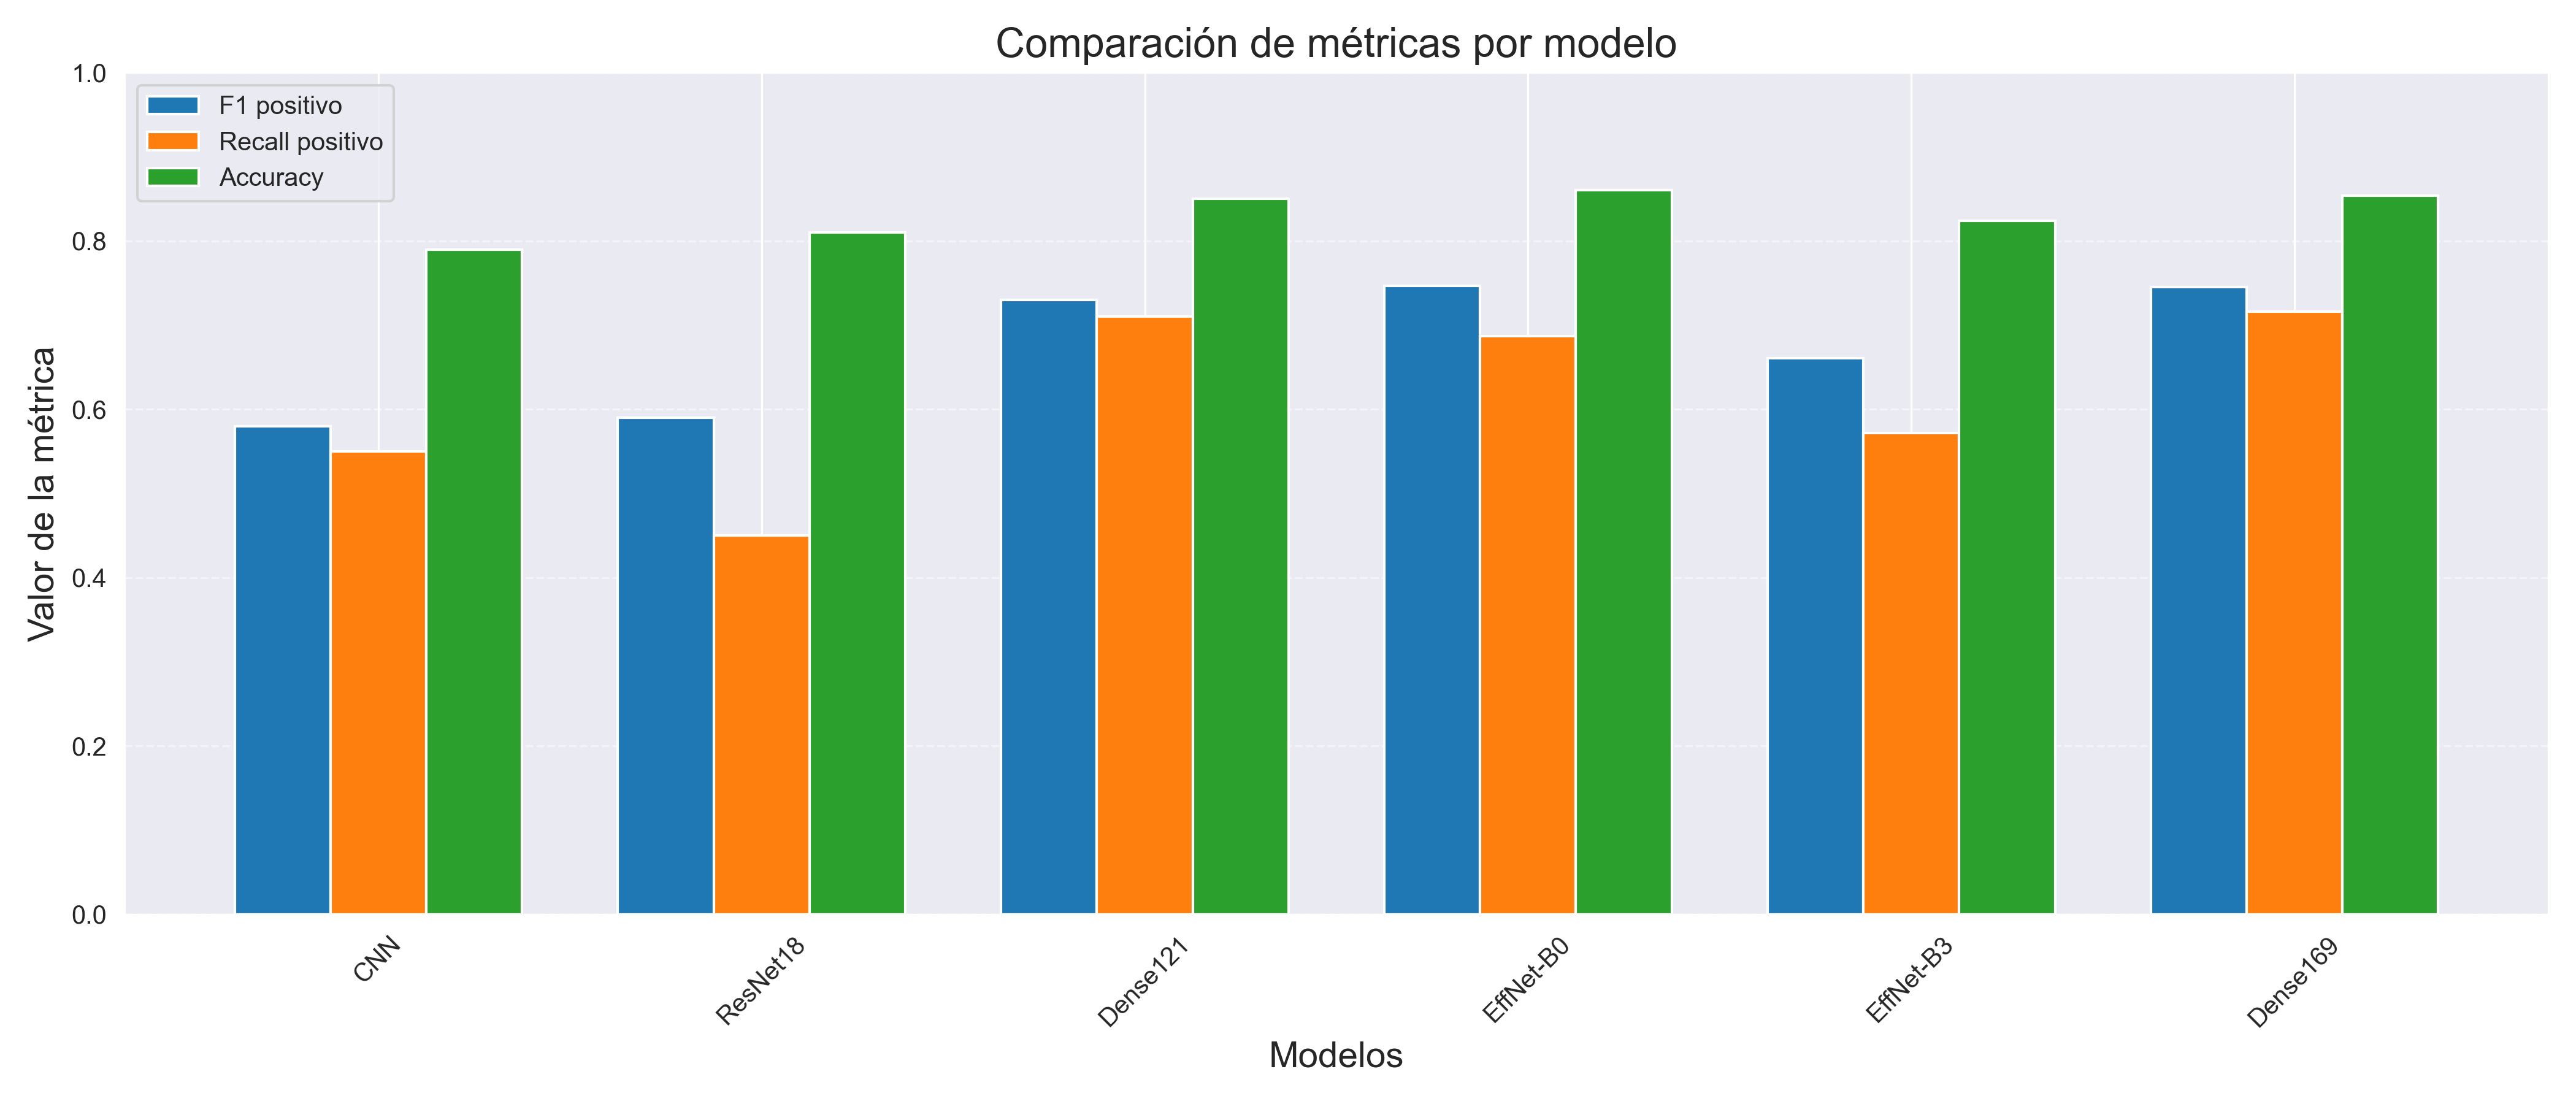
\includegraphics[width=\columnwidth]{images/comparacion_metrica_por_modelo_clasificacion.png}
    \caption{Comparació de les principals mètriques (accuracy, recall positiu i F1-score
    de la classe positiva) per als sis models avaluats.}
    \label{fig:model_comparison}
\end{figure}

Entre els models analitzats, \textbf{EfficientNet-B0} i \textbf{DenseNet-169} destaquen
com les alternatives més equilibrades, assolint valors d’F1-score propers a 0.75 i
accuracies globals superiors al 85\%. Aquest rendiment representa una millora
substancial respecte als enfocaments més simples.

Tanmateix, l’anàlisi del \textit{recall} de la classe positiva —la mètrica més crítica en un
context clínic on els falsos negatius són especialment rellevants— posa de manifest
una limitació important: cap dels models supera el valor de 0.72, i alguns presenten
valors inferiors al 0.60. Això indica que, tot i una bona capacitat per identificar
radiografies normals, els models continuen fallant en una fracció significativa dels
casos amb nòduls pulmonars.

D’aquest anàlisi es desprenen dues conclusions principals: (i) el \textit{transfer learning}
és clarament superior a l’entrenament des de zero en radiologia, especialment en
datasets amb senyals subtils i volum limitat; i (ii) fins i tot els millors models no
capturen encara de manera suficient la complexitat morfològica dels nòduls pulmonars.

En conseqüència, i seguint l’enunciat de la pràctica, es planteja una segona fase
d’innovació metodològica orientada a introduir informació addicional i guiatge
anatòmic, amb l’objectiu de reduir de forma significativa els falsos negatius. La
secció següent descriu aquesta nova proposta basada en preprocessament avançati
canals especialitzats.


% ==================
% # Fase d’Innovació: Motivació i Objectius
% ==================

\section{Fase d’Innovació: Motivació i Objectius}

Tot i l’elevada \textit{accuracy} assolida pels models basats en \textit{transfer learning},
el \textit{recall} de la classe positiva es manté per sota del nivell desitjable per a un
escenari clínic de cribatge. Aquesta limitació és especialment rellevant en la detecció
de nòduls petits o de baix contrast.

Per abordar aquest problema, es planteja una fase d’innovació basada en la introducció
d’una representació multicanal i en el reequilibrat del conjunt de dades mitjançant
augmentació dirigida, amb l’objectiu d’enriquir la informació d’entrada i millorar la
sensibilitat del model. Aquesta aproximació busca apropar el pipeline computacional al
procés de lectura radiològica humana.


\subsection{Augmentació del Dataset per a Classificació}

Per compensar el fort desbalanceig del conjunt de dades original del repte NODE21,
es va aplicar una estratègia d’augmentació orientada exclusivament a la tasca de
classificació binària, sense fer ús de les \textit{bounding boxes}. Atès que l’objectiu
d’aquesta fase no és la detecció sinó la classificació de presència o absència de nòdul,
les transformacions es poden aplicar lliurement sense comprometre anotacions espacials.

L’augmentació es va aplicar únicament sobre la classe positiva, amb l’objectiu
d’incrementar el nombre efectiu de mostres de nòduls i reduir el biaix cap a la classe
majoritària. Es van utilitzar transformacions considerades segures en imatge mèdica,
com soroll i desenfocament gaussià lleus, ajustos de brillantor, contrast i gamma,
CLAHE i petits filtres de reforç de contorns, evitant deformacions geomètriques severes.

Com a resultat, el conjunt de dades va passar d’una distribució inicial de 1476 imatges
positives i 3748 negatives a un dataset completament balancejat amb 3748 mostres per
classe (7496 imatges en total). Aquest reequilibrat permet entrenar models de
classificació més robustos, millorant especialment el \textit{recall} de la classe positiva
i la capacitat de generalització del sistema.


\subsection{Codificació Multicanal: Disseny i Fonament Teòric}

La principal innovació d’aquesta fase consisteix en la construcció d’una representació
\textit{multicanal} de cada radiografia de tòrax, incorporant transformacions clíniques
rellevants que aporten informació complementària a la imatge original. Aquest enfocament
busca aproximar el pipeline computacional al procés de lectura radiològica humana,
on la interpretació no es basa en una única visualització, sinó en l’anàlisi combinada
d’intensitat, contrast i estructura.

En aquesta fase s’han definit tres canals d’entrada:

\begin{itemize}
\item \textbf{Canal 1 – Imatge original normalitzada}: conserva la distribució real
d’intensitats i el context anatòmic complet.
\item \textbf{Canal 2 – CLAHE}: millora el contrast local i realça estructures de baix
relleu, facilitant la identificació de lesions pulmonars poc definides.
\item \textbf{Canal 3 – Contorns Canny}: reforça la informació geomètrica i les fronteres
estructurals, especialment útil per delimitar la perifèria dels nòduls.
\end{itemize}

La Figura~\ref{fig:multicanal_3} mostra un exemple de les tres representacions generades
a partir d’una mateixa radiografia.

\begin{figure}[H]
    \centering
    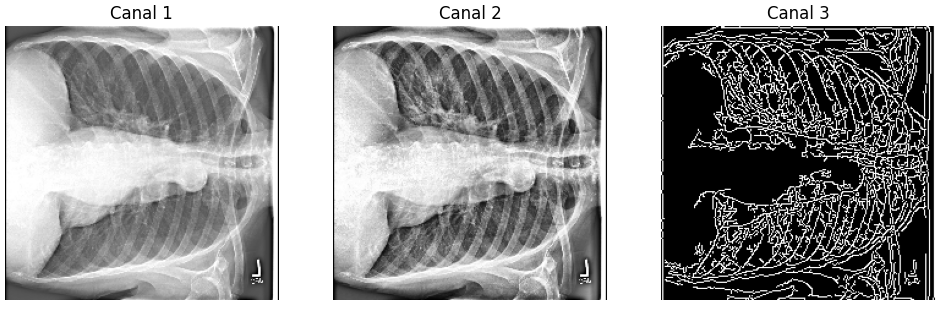
\includegraphics[width=\columnwidth]{images/rx_3_capas.png}
    \caption{Representació multicanal d’una radiografia de tòrax: (1) imatge original
    normalitzada, (2) realç de contrast mitjançant CLAHE i (3) mapa de contorns obtingut
    amb Canny.}
    \label{fig:multicanal_3}
\end{figure}

La combinació d’aquests canals genera una entrada de dimensió $(3 \times 224 \times 224)$
que encapsula informació d’intensitat global, textura local i estructura geomètrica.
Des d’un punt de vista teòric, aquesta codificació defineix un espai de característiques
més discriminatiu que l’ús d’una sola imatge en escala de grisos, permetent que
arquitectures com EfficientNet-B0 explotin de manera més eficient patrons subtils
associats a nòduls pulmonars.


\subsection{Descripció General del Pipeline de Processament i Classificació}

Abans de presentar en detall els resultats de la fase d’innovació, es descriu de manera
sintètica l’estructura general del pipeline de processament i classificació implementat.
L’objectiu és oferir una visió global del flux de dades, destacant els principals blocs
funcionals i el paper de cadascun dins del sistema.

El pipeline es compon de les etapes següents: càrrega i validació de dades, preprocessament
i codificació multicanal, augmentació dirigida del dataset, construcció del dataset
PyTorch, definició del model i entrenament, i finalment l’avaluació quantitativa mitjançant
mètriques estàndard de classificació.

\subsubsection{Càrrega de dades i preprocessament}

Les imatges en format MHA es carreguen mitjançant la llibreria OpenCXR, es normalitzen
a l’interval $[0,1]$ i es redimensionen a $224 \times 224$ píxels. A continuació, es genera
la representació multicanal formada per la imatge original normalitzada, una versió amb
realç de contrast mitjançant CLAHE i un mapa de contorns obtingut amb l’operador Canny.
Aquesta codificació permet aportar informació complementària d’intensitat, textura local
i estructura geomètrica.

\subsubsection{Augmentació i balanceig del dataset}

Per compensar el fort desbalanceig inicial del conjunt de dades NODE21, s’aplica una
estratègia d’augmentació mèdica dirigida exclusivament a la classe positiva (nòdul).
Aquest procés permet obtenir un dataset final perfectament balancejat, reduint el biaix
cap a la classe negativa i millorant la sensibilitat del model.

\subsubsection{Model i configuració d’entrenament}

Com a classificador s’utilitza EfficientNet-B0 preentrenada a ImageNet, adaptada a una
tasca binària mitjançant la substitució de la capa final. L’entrenament es realitza amb
l’optimitzador Adam, funció de pèrdua CrossEntropyLoss, batch size de 32 i execució
en GPU quan està disponible. El bucle d’entrenament calcula la pèrdua mitjana i
l’accuracy per època, mentre que l’avaluació genera l’informe de classificació i la
matriu de confusió sobre el conjunt de test.

\subsubsection{Evolució de l’entrenament}

La Taula~\ref{tab:train_evolution_b0_multicanal} resumeix l’evolució de la pèrdua i
l’accuracy durant les cinc èpoques d’entrenament. S’observa una reducció progressiva
de la pèrdua i una millora estable del rendiment, sense indicis clars de sobreajust.

\begin{table}[H]
\caption{Evolució de la pèrdua i l’accuracy d’entrenament del model EfficientNet-B0 multicanal}
\label{tab:train_evolution_b0_multicanal}
\centering
\footnotesize
\setlength{\tabcolsep}{4pt}
\begin{tabular}{ccc}
\toprule
\textbf{Època} & \textbf{Loss train} & \textbf{Accuracy train} \\
\midrule
1 & 0.3335 & 0.8500 \\
2 & 0.1827 & 0.9292 \\
3 & 0.1435 & 0.9435 \\
4 & 0.1140 & 0.9610 \\
5 & 0.1057 & 0.9596 \\
\bottomrule
\end{tabular}
\end{table}

La Figura~\ref{fig:training_curves_b0_multicanal} mostra l’evolució conjunta de la
pèrdua i de l’accuracy durant l’entrenament.

\begin{figure}[H]
    \centering
    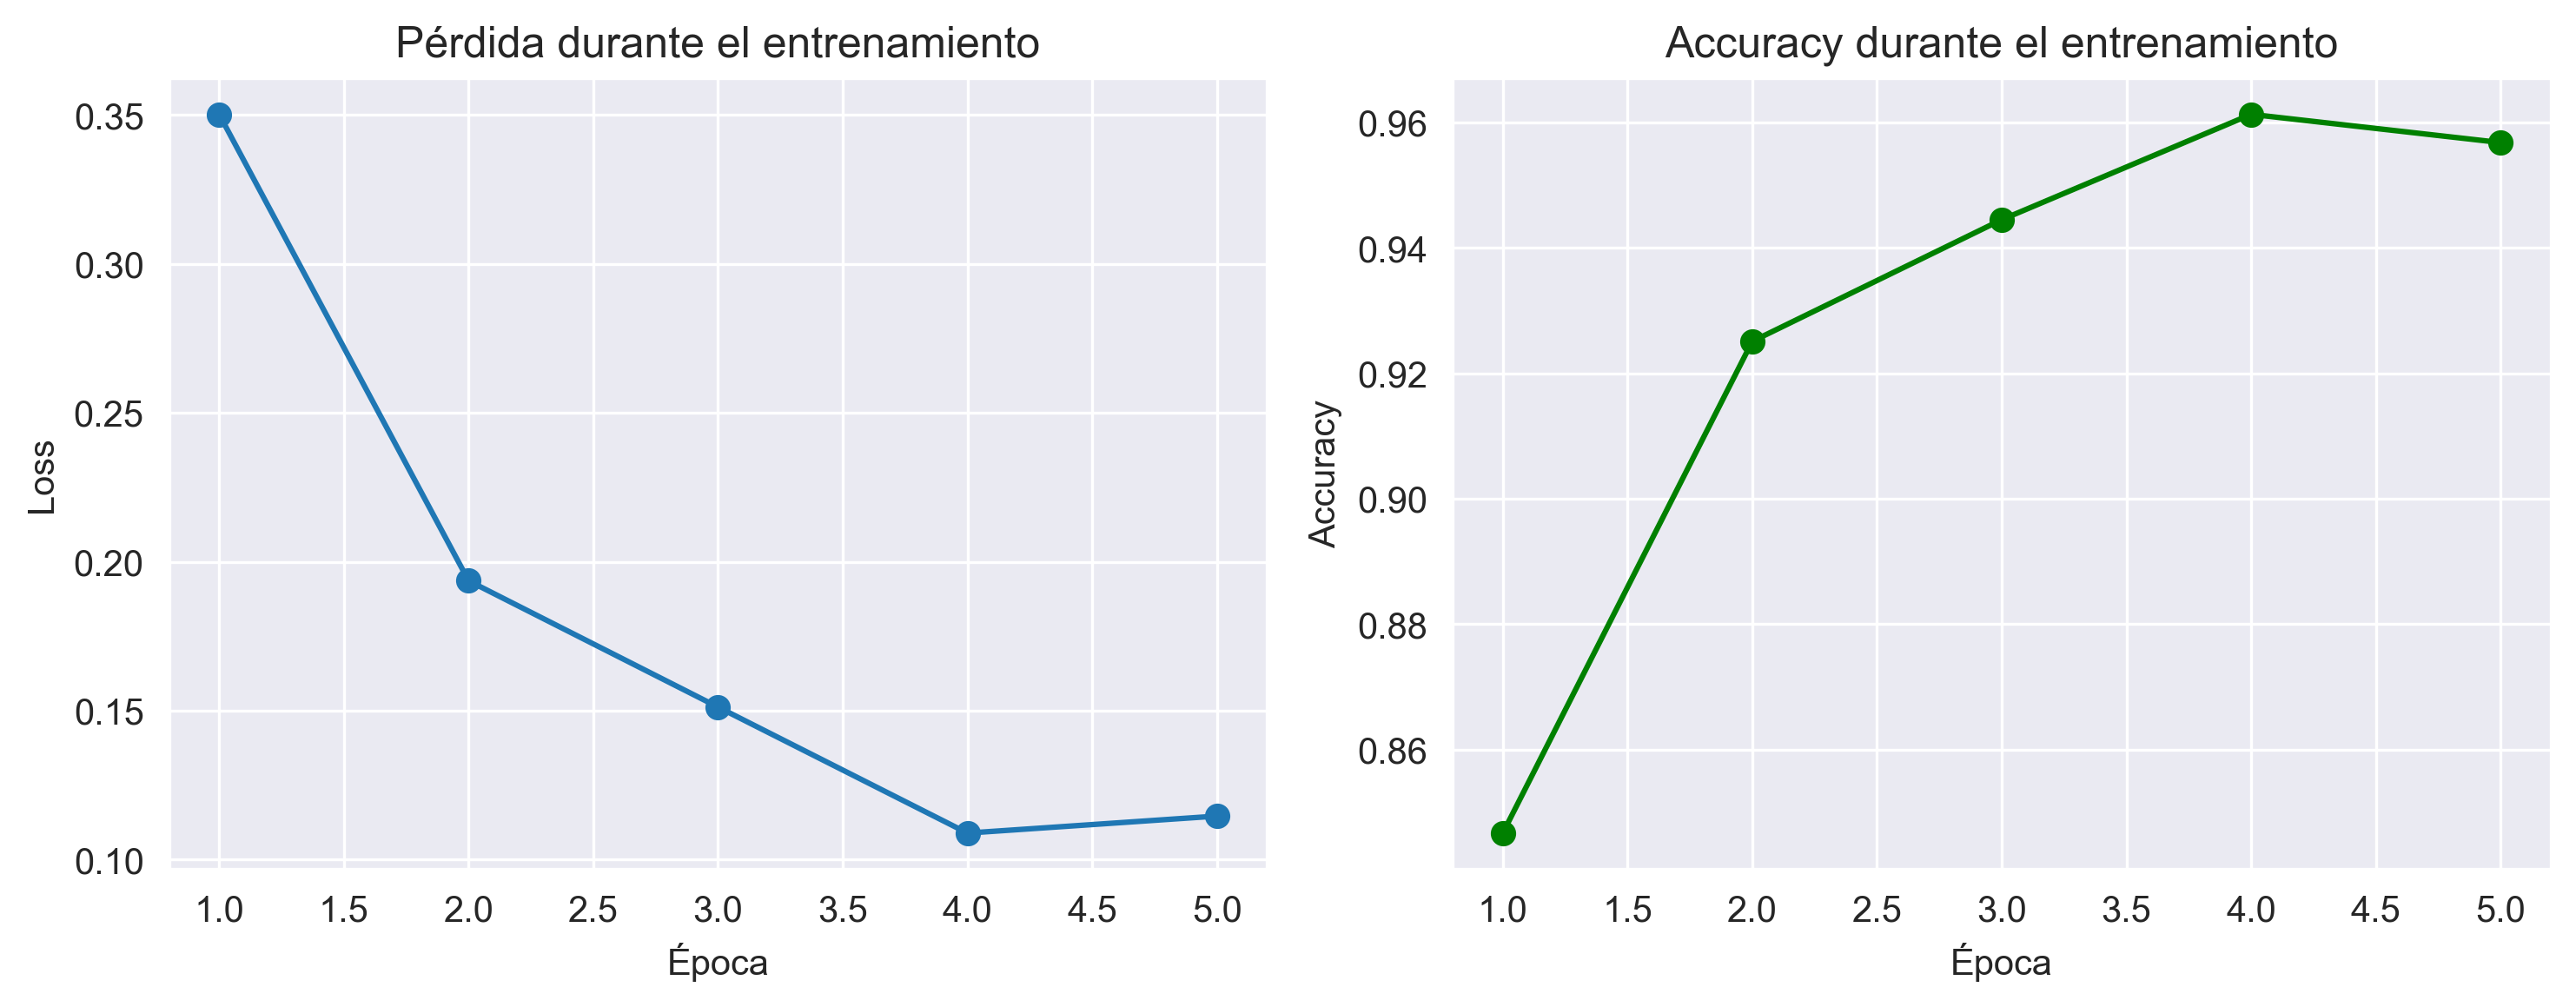
\includegraphics[width=\columnwidth]{images/efficientnet_b0_training_curves.png}
    \caption{Evolució de la pèrdua (loss) i de l’accuracy durant l’entrenament del model
    EfficientNet-B0 multicanal.}
    \label{fig:training_curves_b0_multicanal}
\end{figure}

\subsubsection{Resultats sobre el conjunt de test}

L’avaluació final es realitza sobre un conjunt de test de 1\,045 imatges. El model assoleix
una accuracy global del 97.03\%, amb un excel·lent equilibri entre precisió i sensibilitat
per a ambdues classes.

La Taula~\ref{tab:confusion_matrix_b0_multicanal} mostra la matriu de confusió
corresponent.

\begin{table}[H]
\caption{Matriu de confusió del model EfficientNet-B0 multicanal sobre el conjunt de test}
\label{tab:confusion_matrix_b0_multicanal}
\centering
\footnotesize
\begin{tabular}{lcc}
\toprule
 & \textbf{Pred. 0} & \textbf{Pred. 1} \\
\midrule
\textbf{Classe 0} & 710 & 22 \\
\textbf{Classe 1} & 9   & 304 \\
\bottomrule
\end{tabular}
\end{table}

La representació gràfica de la matriu de confusió es mostra a la
Figura~\ref{fig:confusion_matrix_b0_multicanal}, on es visualitza clarament el baix nombre
de falsos negatius i falsos positius.

\begin{figure}[H]
    \centering
    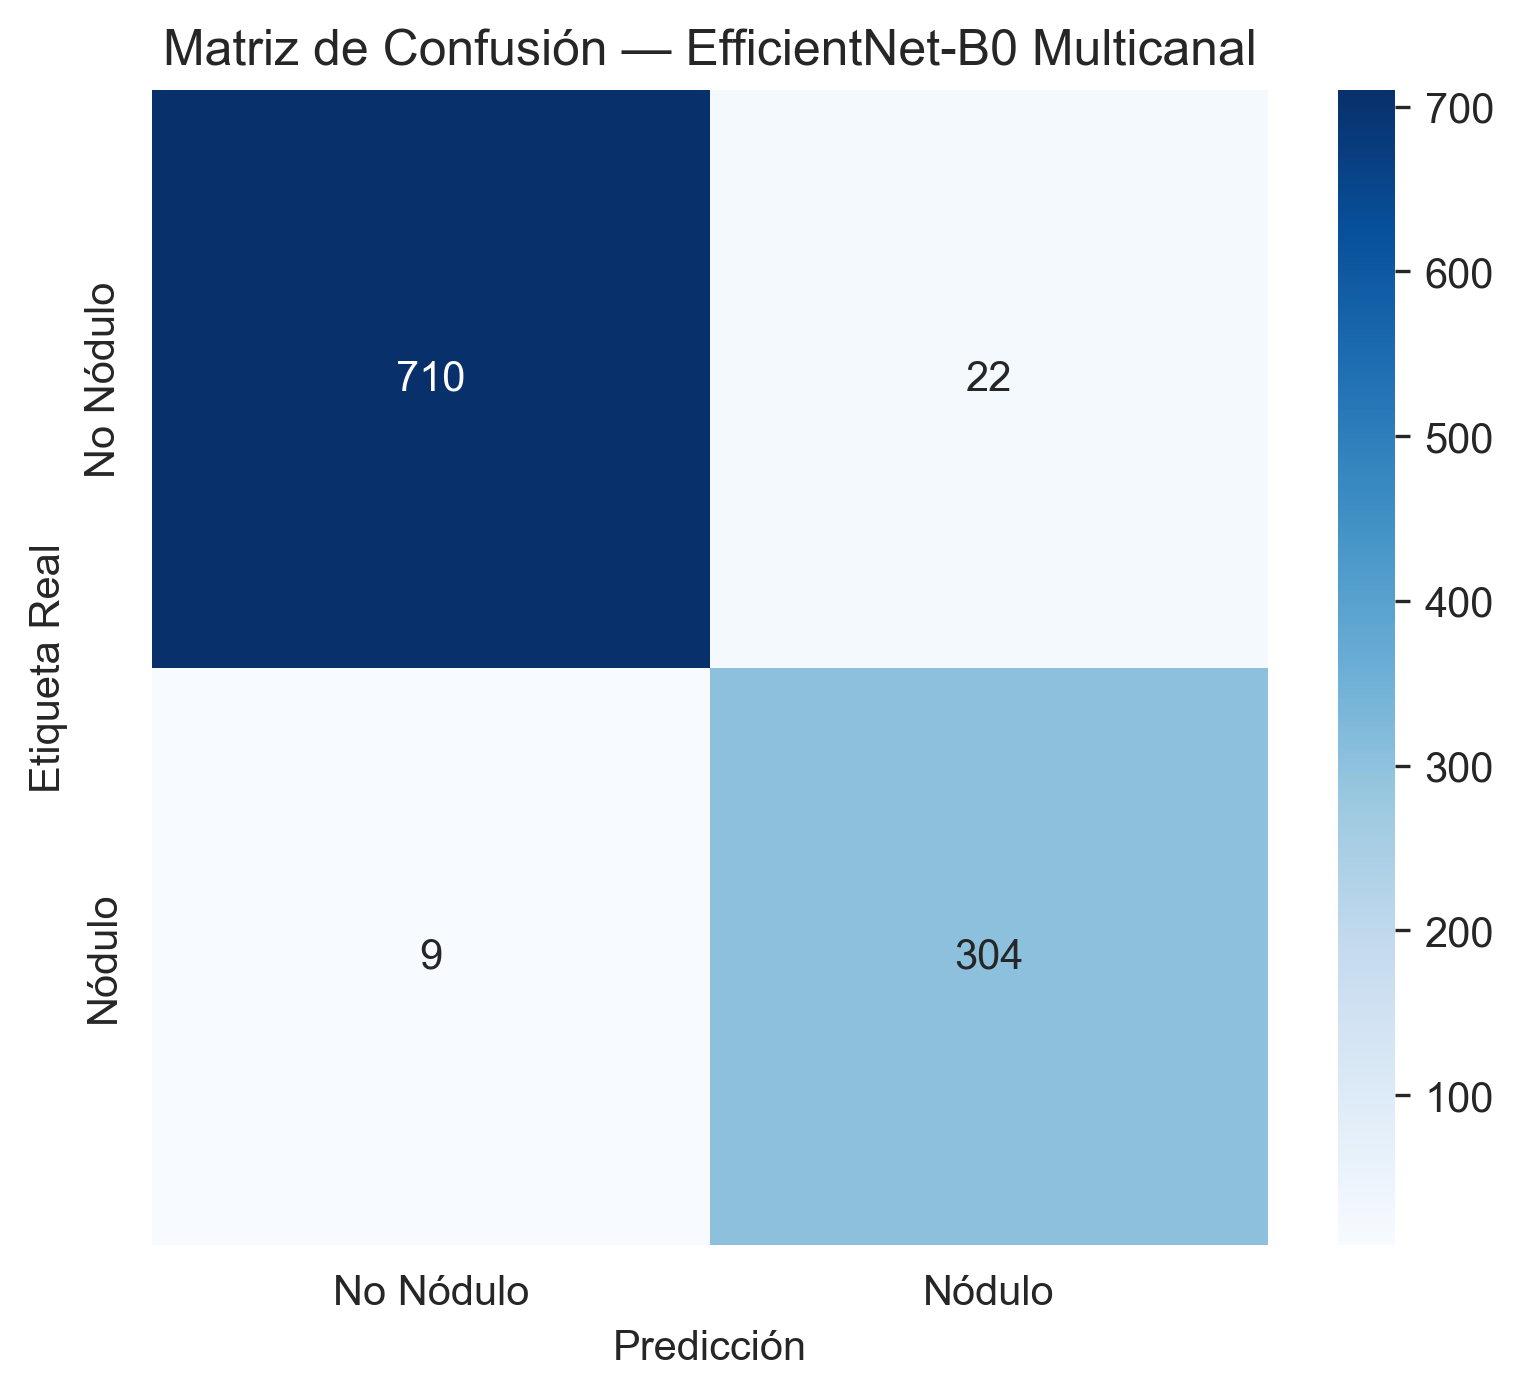
\includegraphics[width=\columnwidth]{images/efficientnet_b0_confusion_matrix.png}
    \caption{Matriu de confusió del model EfficientNet-B0 multicanal sobre el conjunt de test.}
    \label{fig:confusion_matrix_b0_multicanal}
\end{figure}

\subsubsection{Discussió}

Els resultats confirmen que la combinació de codificació multicanal, dataset balancejat
i EfficientNet-B0 permet assolir un rendiment molt elevat, especialment en termes de
recall de la classe positiva (97.12\%). Aquest comportament és especialment rellevant
en un context de cribratge clínic, on la minimització de falsos negatius és crítica.
En conjunt, aquest pipeline es consolida com la millor estratègia de classificació
avaluada fins al moment i constitueix la base per a les fases posteriors d’estudi d’ablació
i anàlisi comparativa.

\subsection{Model definitiu: extensió del model multicanal de 3 a 4 canals}

En l’experiment anterior es va utilitzar una representació multicanal formada per tres
canals derivats de cada radiografia de tòrax: la imatge original normalitzada, una versió
amb realç de contrast mitjançant CLAHE i un mapa de contorns obtingut amb el detector
de Canny. Aquesta aproximació ja va permetre millorar de manera notable la sensibilitat
en la detecció de nòduls pulmonars, especialment en lesions petites o de baix contrast.

No obstant això, l’anàlisi qualitativa dels errors i la revisió del procés de lectura clínica
van posar de manifest que la detecció de nòduls no depèn únicament del contrast i del
contorn, sinó també de la presència de textures fines i microirregularitats en el parènquima
pulmonar. Per aquest motiu, es va decidir enriquir la representació multicanal incorporant
un quart canal basat en la tècnica d’\textit{Unsharp Mask}.

Aquesta operació realça les components d’alta freqüència de la imatge i permet destacar
vores suaus, textures fines i canvis estructurals subtils, sovint rellevants en la pràctica
radiològica. El model definitiu treballa, per tant, amb quatre canals d’entrada:

\begin{itemize}
\item \textbf{Canal 1:} imatge original normalitzada (informació d’intensitat global).
\item \textbf{Canal 2:} CLAHE (realç de contrast local i estructures de baix relleu).
\item \textbf{Canal 3:} contorns Canny (informació geomètrica i vores ben definides).
\item \textbf{Canal 4:} Unsharp Mask (textures fines i contorns suaus realçats).
\end{itemize}

Aquesta combinació aproxima de manera més fidel el procés cognitiu del radiòleg, que
integra simultàniament informació de contrast, estructura i textura per decidir la presència
d’un nòdul. La Figura~\ref{fig:four_channel_example} mostra un exemple de les quatre
representacions utilitzades.

\begin{figure}[H]
    \centering
    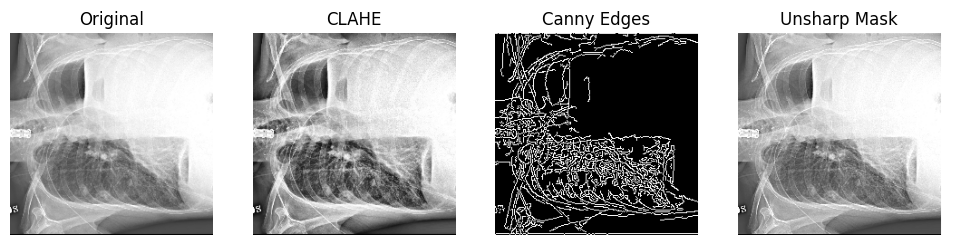
\includegraphics[width=\columnwidth]{images/rx_4_capas.png}
    \caption{Visualització dels quatre canals emprats en el model multicanal: (1) imatge
    original normalitzada, (2) CLAHE, (3) detecció de contorns Canny i (4) Unsharp Mask.}
    \label{fig:four_channel_example}
\end{figure}

L’augmentació de dades s’ha adaptat mínimament per operar sobre tensors de quatre
canals, mantenint exclusivament transformacions considerades clínicament segures
(flips horitzontals, rotacions suaus i soroll gaussià lleu). La resta del pipeline
(dataset balancejat, arquitectura EfficientNet-B0 i estratègia d’entrenament) es manté
idèntica a l’experiment anterior per tal d’aïllar l’efecte del quart canal.

El conjunt de dades final es divideix aproximadament en un 80\% per entrenament i un
20\% per test. El conjunt de test conté 1\,500 imatges, amb una distribució gairebé
equilibrada entre classes (751 sense nòdul i 749 amb nòdul).

\subsection{Resultats quantitatius}

La Taula~\ref{tab:classification_report_b0_4ch} resumeix el \textit{classification report}
obtingut sobre el conjunt de test. El model assoleix una accuracy global del 98.07\%,
amb valors de precisió, recall i F1-score molt elevats i equilibrats entre classes.

\begin{table}[H]
\caption{Resultats del model EfficientNet-B0 multicanal (4 canals) sobre el conjunt de test}
\label{tab:classification_report_b0_4ch}
\centering
\footnotesize
\setlength{\tabcolsep}{4pt}
\begin{tabular}{lcccc}
\toprule
\textbf{Classe} & \textbf{Prec.} & \textbf{Rec.} & \textbf{F1} & \textbf{Sup.} \\
\midrule
0 (no nòdul) & 0.9892 & 0.9720 & 0.9805 & 751 \\
1 (nòdul)   & 0.9724 & 0.9893 & 0.9808 & 749 \\
\midrule
Accuracy     & \multicolumn{4}{c}{0.9807} \\
Macro avg    & 0.9808 & 0.9807 & 0.9807 & 1500 \\
Weighted avg & 0.9808 & 0.9807 & 0.9807 & 1500 \\
\bottomrule
\end{tabular}
\end{table}

\subsection{Matriu de confusió}

La Taula~\ref{tab:confusion_matrix_b0_4ch} mostra els valors exactes de la matriu de
confusió, mentre que la Figura~\ref{fig:confusion_matrix_b0_4ch} en presenta la
representació gràfica.

\begin{table}[H]
\caption{Matriu de confusió del model EfficientNet-B0 multicanal (4 canals)}
\label{tab:confusion_matrix_b0_4ch}
\centering
\footnotesize
\begin{tabular}{lcc}
\toprule
 & \textbf{Pred. 0} & \textbf{Pred. 1} \\
\midrule
\textbf{Classe 0} & 730 & 21 \\
\textbf{Classe 1} & 8   & 741 \\
\bottomrule
\end{tabular}
\end{table}

\begin{figure}[H]
    \centering
    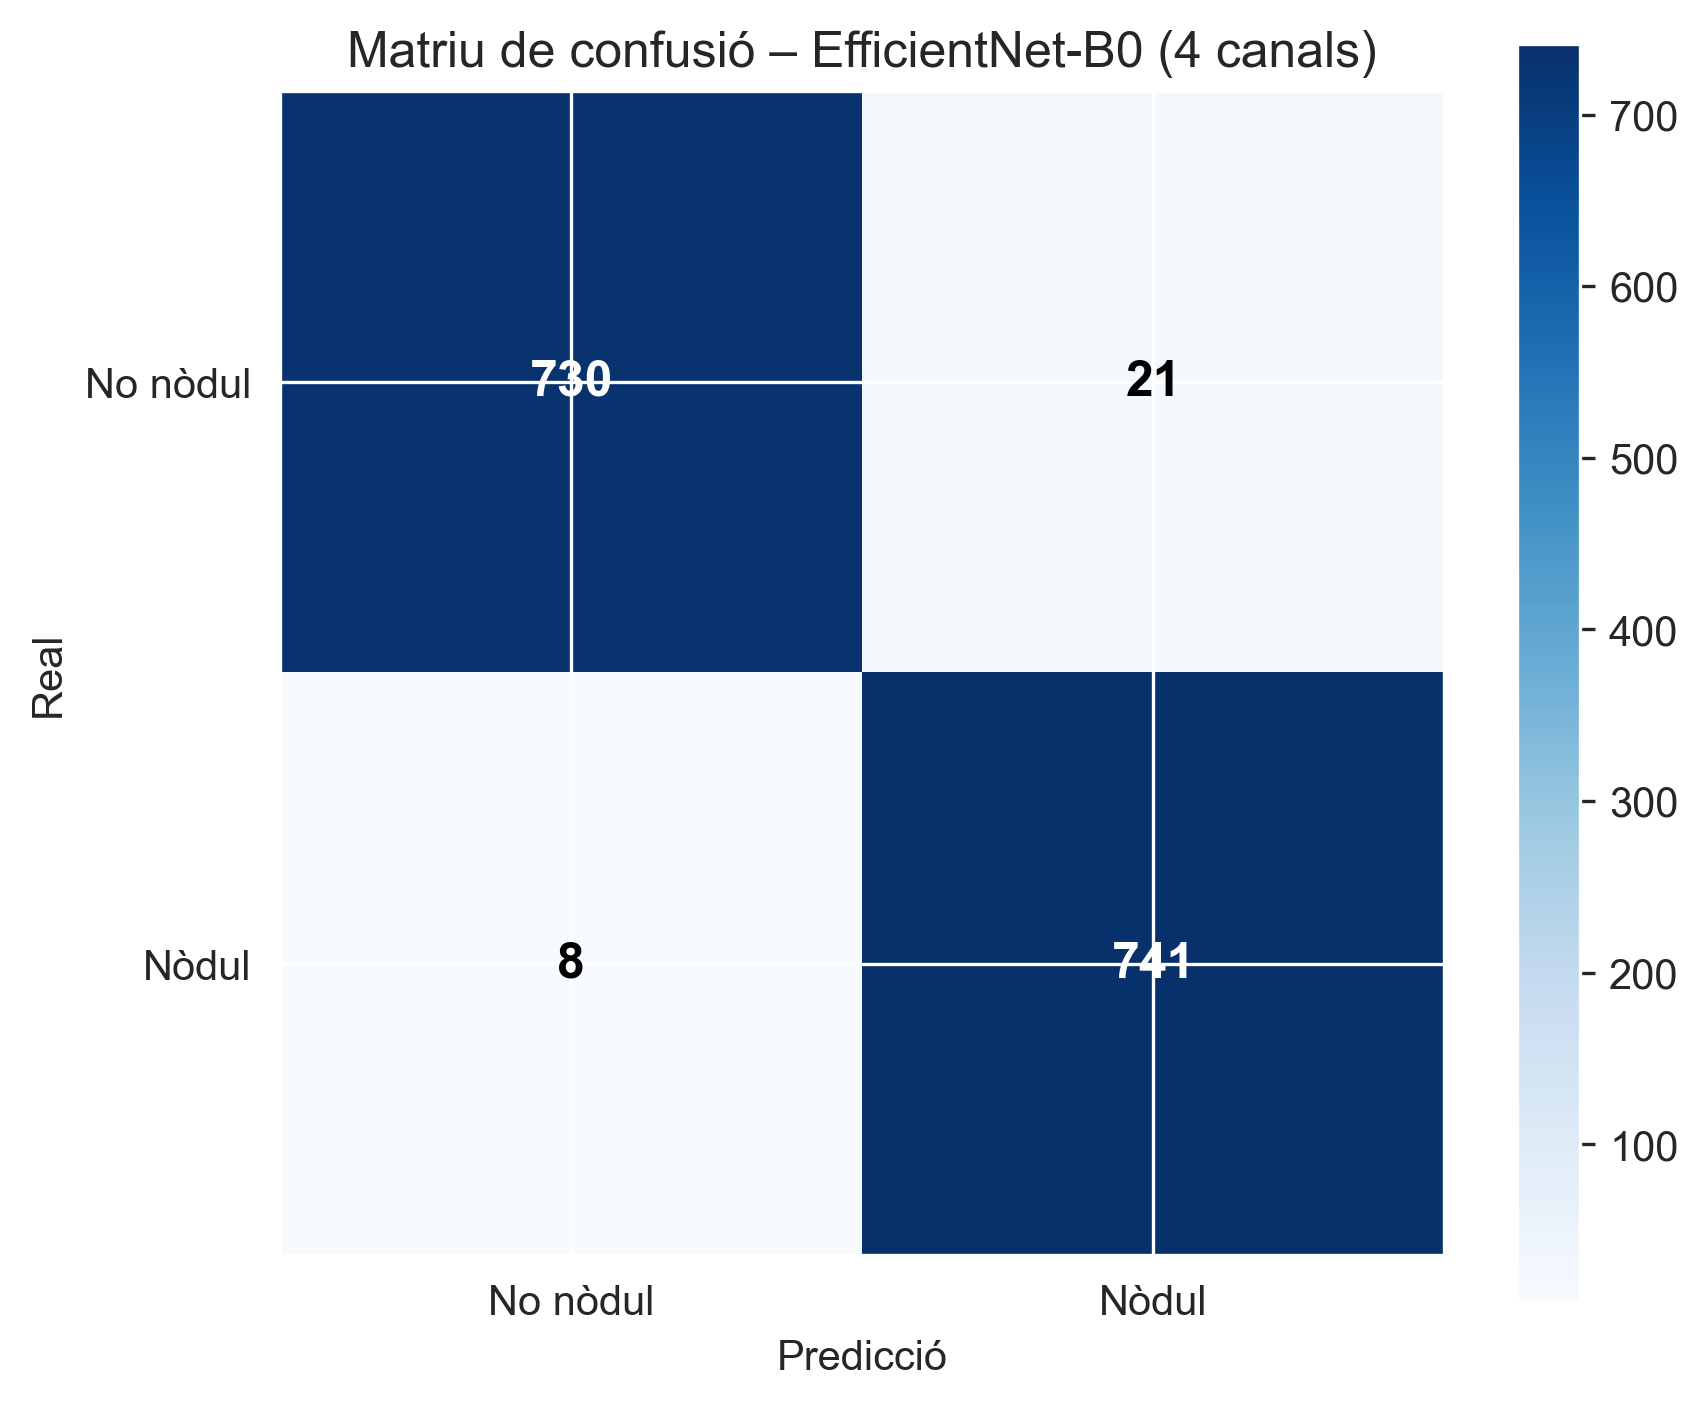
\includegraphics[width=\columnwidth]{images/confusion_matrix_efficientnetb0_4canales.png}
    \caption{Matriu de confusió del model EfficientNet-B0 multicanal amb quatre canals.}
    \label{fig:confusion_matrix_b0_4ch}
\end{figure}

Els falsos negatius representen només l’1.1\% dels nòduls reals, mentre que els falsos
positius corresponen al 2.8\% de les radiografies normals, valors especialment adequats
per a un sistema de suport al cribratge clínic.

\subsection{Evolució de l’entrenament}

La Figura~\ref{fig:effb0_4c_training} mostra l’evolució de la pèrdua i de l’accuracy
durant les 20 èpoques d’entrenament. La pèrdua decreix de forma progressiva, mentre
que l’accuracy supera el 97\% a partir de la desena època, sense evidència clara de
sobreajust.

\begin{figure}[H]
    \centering
    \begin{subfigure}[H]{0.48\columnwidth}
        \centering
        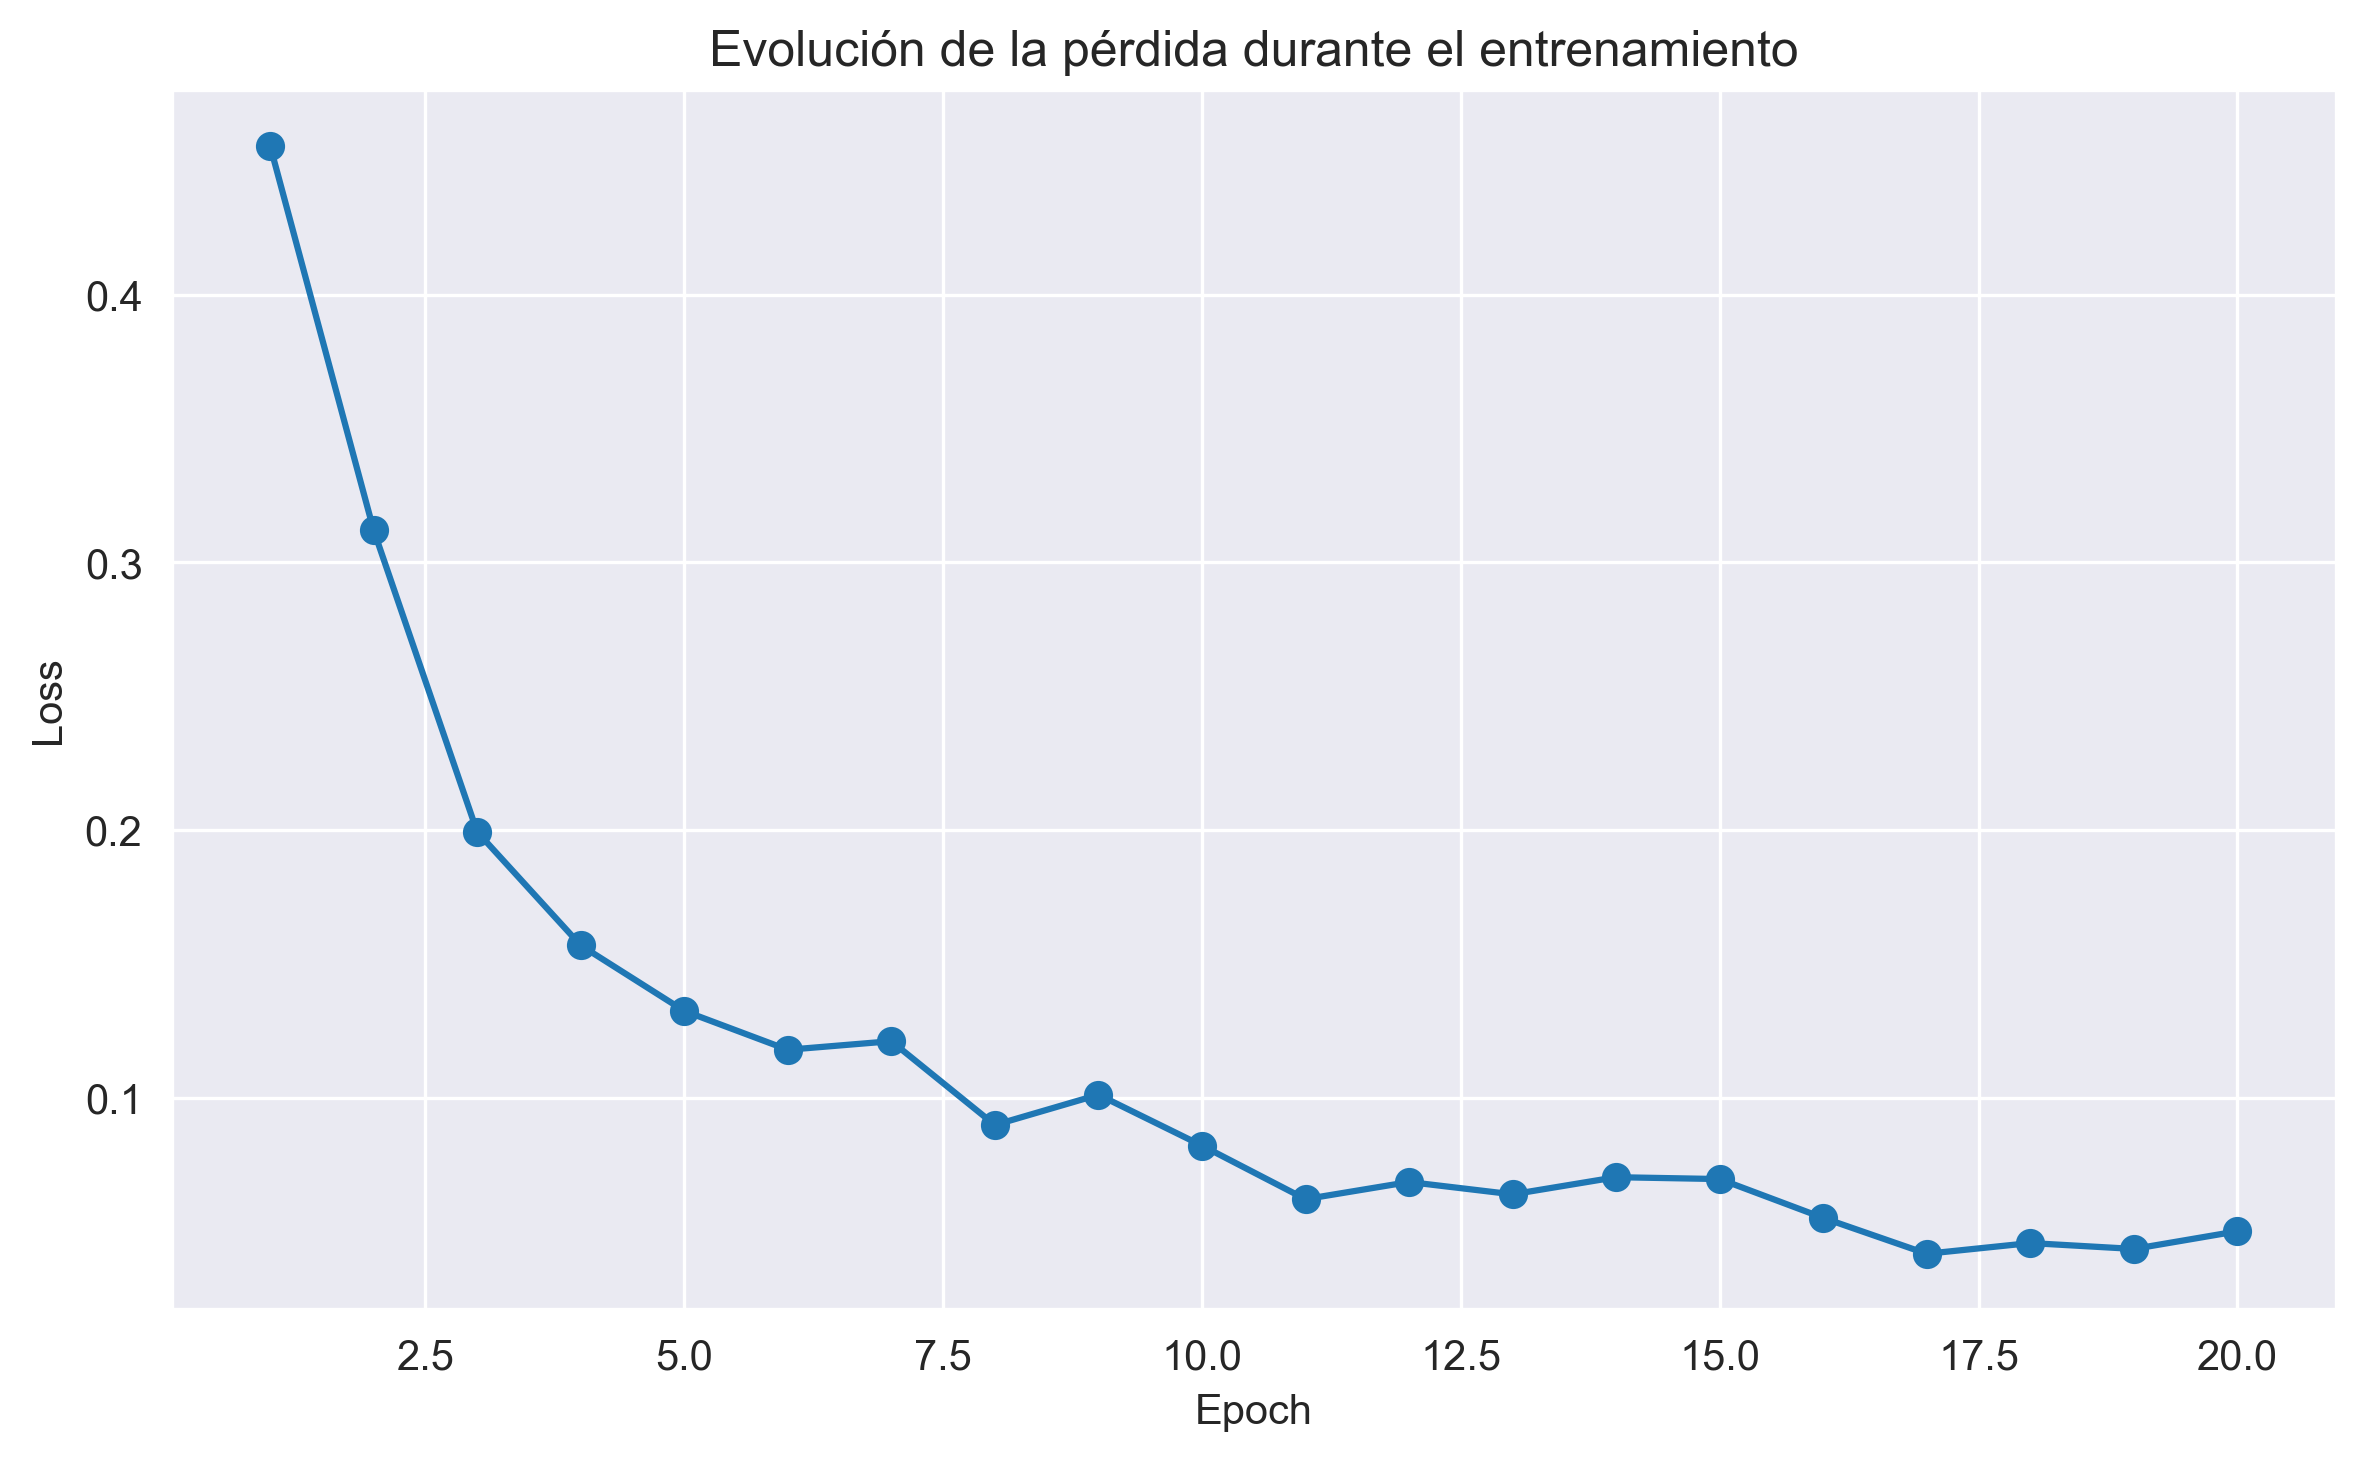
\includegraphics[width=\linewidth]{images/loss_final_efficientnetb0_4canales.png}
        \caption{Evolució de la pèrdua (\emph{loss}).}
        \label{fig:effb0_4c_loss}
    \end{subfigure}
    \hfill
    \begin{subfigure}[H]{0.48\columnwidth}
        \centering
        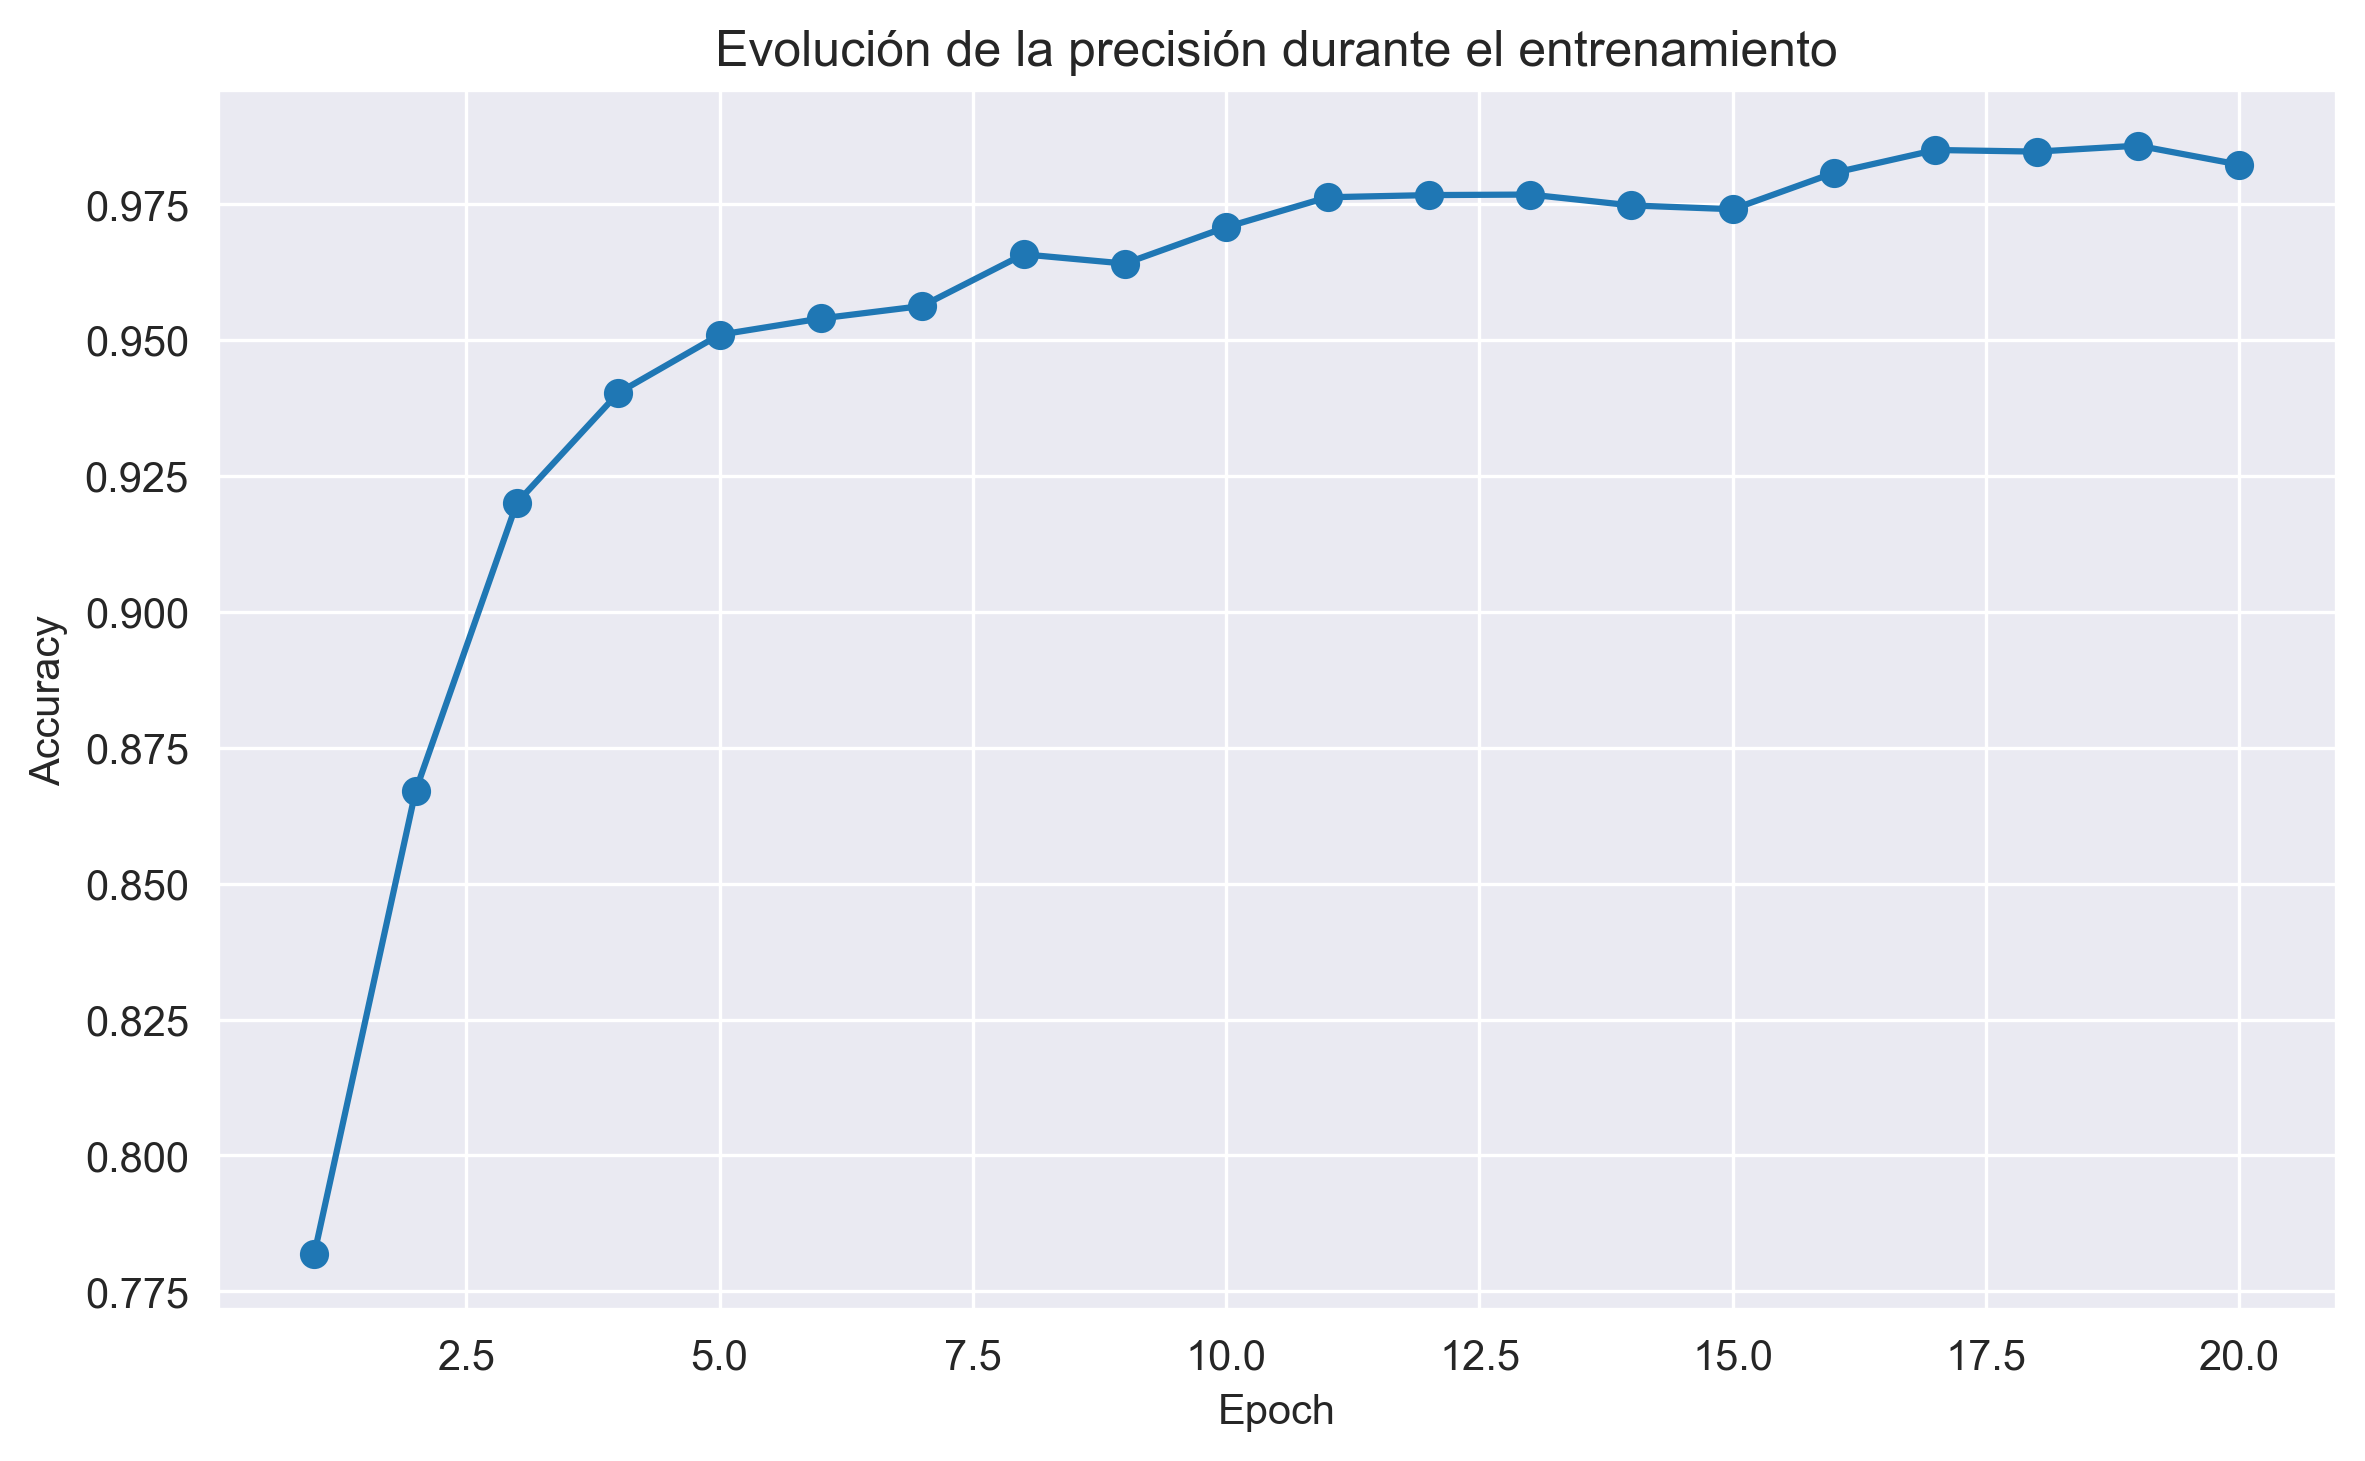
\includegraphics[width=\linewidth]{images/accuracy_final_efficientnetb0_4canales.png}
        \caption{Evolució de l'exactitud (\emph{accuracy}).}
        \label{fig:effb0_4c_accuracy}
    \end{subfigure}

    \caption{Evolució de la pèrdua (\emph{loss}) i de l'exactitud (\emph{accuracy}) durant les 20 èpoques d'entrenament del model EfficientNet-B0 multicanal amb quatre canals d'entrada.}
    \label{fig:effb0_4c_training}
\end{figure}

\subsection{Discussió final}

La comparació amb els models avaluats en fases prèvies confirma que
EfficientNet-B0 multicanal amb quatre canals i dataset balancejat ofereix el millor
compromís global entre sensibilitat, especificitat i estabilitat d’entrenament.
Aquesta arquitectura constitueix el pipeline definitiu del present estudi i estableix
una base sòlida per a futures extensions, com ara estudis d’ablació detallats o la
integració amb models de detecció i segmentació.

% ==================
% # Fase d’Innovació: Motivació i Objectius
% ==================

\section{Estudi d’Ablació del Pipeline Multicanal}

Un cop fixada l’arquitectura EfficientNet-B0 i el procediment d’entrenament, es va
realitzar un estudi d’ablació amb l’objectiu d’analitzar de manera rigorosa la contribució
individual de cada canal afegit al pipeline multicanal. Tots els experiments es van dur
a terme mantenint constants l’arquitectura, els hiperparàmetres, l’esquema
d’entrenament i el procediment d’avaluació, garantint així la comparabilitat directa
dels resultats. Per a les configuracions més rellevants, els experiments es van repetir
utilitzant un dataset explícitament balancejat per analitzar la interacció entre
codificació multicanal i distribució de classes.

\begin{table}[H]
\centering
\scriptsize
\renewcommand{\arraystretch}{1.1}
\begin{tabularx}{\columnwidth}{c X c c c c}
\toprule
\textbf{Can.} & \textbf{Configuració} & \textbf{Acc.} & \textbf{Rec.(1)} & \textbf{FN} & \textbf{FP} \\
\midrule
1 & Original & 0.9667 & 0.9573 & 32 & 18 \\
1 & Canny & 0.9173 & 0.8478 & 114 & 10 \\
1 & Unsharp & 0.9673 & 0.9546 & 34 & 15 \\
2 & Orig. + CLAHE & 0.9813 & 0.9933 & 5 & 23 \\
2 & Orig. + CLAHE (balencejat) & \textbf{0.9884} & \textbf{0.9955} & \textbf{4} & 15 \\
3 & Orig. + CLAHE + Canny & 0.9713 & 0.9693 & 23 & 20 \\
3 & Orig. + CLAHE + Unsharp & 0.9800 & 0.9706 & 22 & \textbf{8} \\
3 & Orig. + CLAHE + Unsharp (balencejat) & \textbf{0.9884} & 0.9933 & 6 & 13 \\
4 & Orig. + CLAHE + Canny + Unsharp & 0.9813 & 0.9800 & 15 & 13 \\
4 & Orig. + CLAHE + Canny + Unsharp (balencejat) & 0.9835 & 0.9821 & 16 & 11 \\
\bottomrule
\end{tabularx}
\caption{Resultats de l’estudi d’ablació del pipeline multicanal amb EfficientNet-B0.}
\label{tab:ablation_results}
\end{table}

Les configuracions avaluades inclouen representacions monocanal (Original, Canny i
Unsharp Mask), combinacions de dos canals (Original + CLAHE), tres canals
(Original + CLAHE amb Canny o Unsharp Mask) i quatre canals
(Original + CLAHE + Canny + Unsharp Mask). El rendiment s’ha avaluat mitjançant
l’accuracy global, el \textit{recall} de la classe positiva, i el nombre de falsos
negatius (FN) i falsos positius (FP), mètriques especialment rellevants en un context
clínic (Taula~\ref{tab:ablation_results}).




Les configuracions monocanal estableixen una línia base raonable, però presenten un
nombre no negligible de falsos negatius. L’ús exclusiu de Canny mostra el pitjor
rendiment global, amb una caiguda pronunciada del \textit{recall}, confirmant que la
detecció de vores dures elimina informació clínica rellevant associada a variacions
suaus de densitat. El canal Unsharp Mask, utilitzat de forma aïllada, no aporta una
millora significativa de la sensibilitat.

La incorporació de CLAHE com a segon canal representa el factor més determinant de
millora del pipeline. La configuració de dos canals (Original + CLAHE) assoleix els
valors més elevats de \textit{recall}, especialment quan s’utilitza un dataset
balancejat, amb només 4 falsos negatius. Aquest resultat evidencia que el realç de
contrast local és clau per a la detecció de nòduls de baix contrast.

L’addició de Canny com a tercer canal tendeix a degradar la sensibilitat, mentre que
la combinació de tres canals basada en Original + CLAHE + Unsharp Mask ofereix un
compromís més equilibrat, mantenint una sensibilitat elevada i reduint el nombre de
falsos positius. La configuració de quatre canals presenta un comportament estable,
però no supera les configuracions més simples en termes de \textit{recall}.

En conclusió, l’estudi d’ablació demostra que CLAHE és el component fonamental del
pipeline multicanal i que el balanç del dataset reforça de manera significativa els
seus beneficis. Des d’un punt de vista clínic, la configuració de \textbf{dos canals
(Original + CLAHE, dataset balancejat)} és especialment adequada per a escenaris de
cribratge, mentre que la configuració de \textbf{tres canals (Original + CLAHE +
Unsharp Mask)} ofereix un compromís més equilibrat entre sensibilitat i especificitat.


\section{Anàlisi d’Explicabilitat (XAI): Aproximació Exploradora}

En aquesta fase del treball s’ha realitzat una primera aproximació
\textit{experimental} a tècniques d’explicabilitat (\textit{Explainable Artificial Intelligence}, XAI),
amb l’objectiu d’introduir i comprendre els conceptes bàsics associats a la
interpretació de models d’aprenentatge profund aplicats a imatges mèdiques.

Cal remarcar que aquesta anàlisi \textbf{no té com a finalitat la validació clínica
del comportament del model}, sinó que s’emmarca dins d’un context formatiu.
L’objectiu principal ha estat familiaritzar-se amb el concepte d’explicabilitat
post-hoc, entendre què significa explicar una predicció i analitzar de manera
qualitativa el funcionament intern del model. Aquesta aproximació segueix els
conceptes introduïts a l’assignatura d’Aprenentatge Automàtic i les explicacions
proporcionades pel professor \textbf{Miquel Miró} durant les sessions docents.

Per a dur a terme aquest estudi explorador s’ha utilitzat la llibreria
\textbf{Captum}, desenvolupada sobre PyTorch, que proporciona implementacions
estàndard i àmpliament acceptades de tècniques XAI. Concretament, s’ha aplicat el
mètode \textbf{Integrated Gradients}, una tècnica post-hoc basada en gradients que
permet estimar la contribució de cada píxel de la imatge d’entrada a la decisió
final del classificador.

L’anàlisi d’explicabilitat s’ha realitzat sobre el model de classificació
multicanal desenvolupat en aquest treball, considerant els quatre canals
d’entrada utilitzats: imatge original, CLAHE, Canny i Unsharp Mask. Les
atribucions obtingudes mitjançant Integrated Gradients s’han analitzat tant de
manera individual per canal com de forma combinada, amb l’objectiu d’observar
quines representacions d’entrada contribueixen en major mesura a la predicció
final del model.

Addicionalment, s’ha calculat una mesura quantitativa senzilla de contribució
relativa per canal, basada en la suma del valor absolut de les atribucions.
Aquesta mètrica s’ha utilitzat exclusivament amb finalitats exploradores i
interpretatives, i \textbf{no s’ha de considerar com una mesura causal ni com una
validació formal del model}, sinó com una eina per facilitar la comprensió del
comportament del classificador.

En conjunt, aquesta secció pretén introduir el concepte d’explicabilitat dins del
projecte i establir una base conceptual inicial sobre l’ús de tècniques XAI en
models de visió per computador aplicats a l’àmbit mèdic. Tot i que els
coneixements en explicabilitat són encara limitats, aquesta aproximació ha
permès adquirir una primera visió pràctica d’aquestes tècniques i obre la porta
a futurs treballs on l’XAI pugui tenir un paper més central i rigorós.


\subsection{Anàlisi qualitativa de l’explicabilitat mitjançant Integrated Gradients}

\begin{figure}[H]
    \centering
    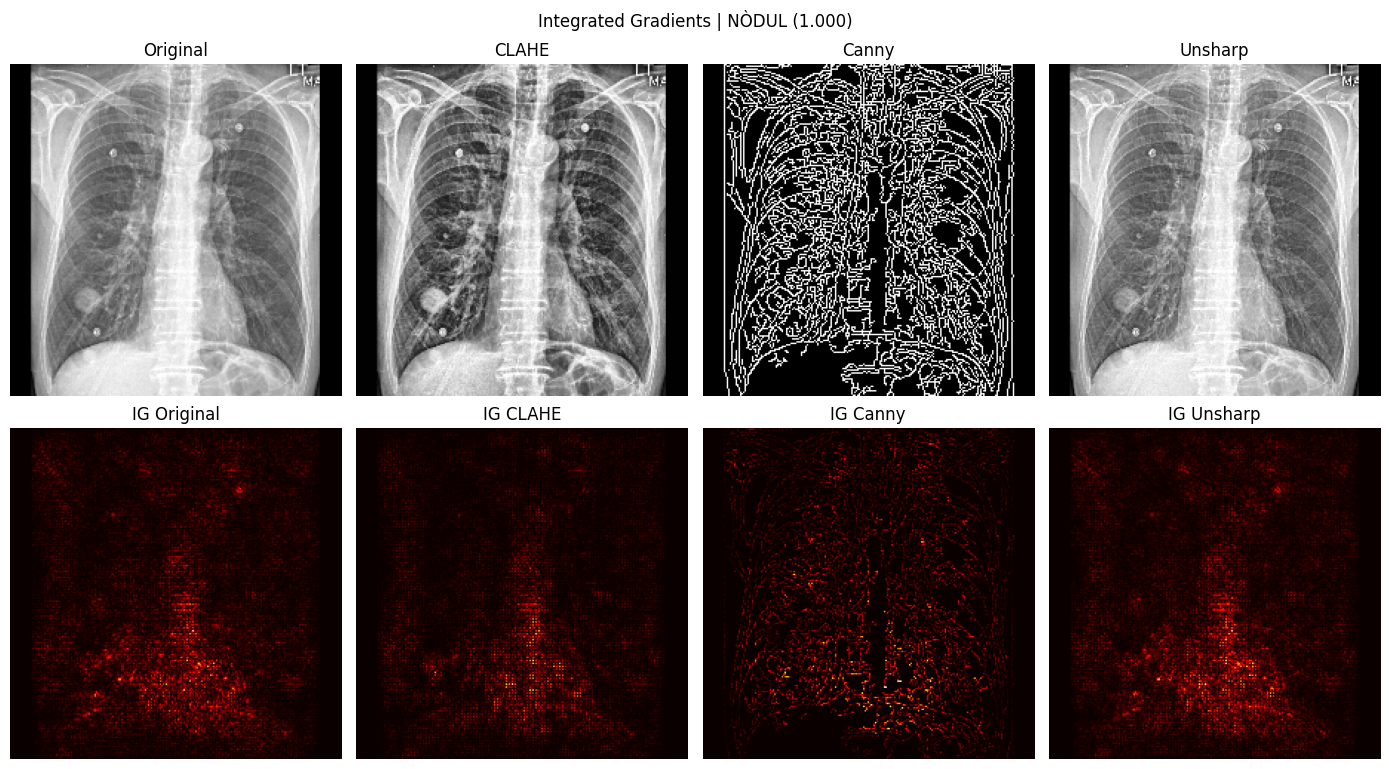
\includegraphics[width=0.45\textwidth]{images/ig_multicanal_example.png}
    \caption{Mapes d’atribució obtinguts amb Integrated Gradients per als quatre canals
    d’entrada del model de classificació multicanal.}
    \label{fig:ig_multicanal}
\end{figure}

La Figura~\ref{fig:ig_multicanal} mostra els resultats de l’anàlisi
d’explicabilitat obtinguts mitjançant el mètode \textit{Integrated Gradients}
aplicat a un cas classificat com a nòdul pulmonar. A la fila superior es
presenten les quatre representacions d’entrada utilitzades pel model
(classificació multicanal): imatge original, imatge amb realce de contrast
local (CLAHE), detecció de contorns mitjançant Canny i imatge amb reforç de
detall (Unsharp Mask). A la fila inferior es mostren els corresponents mapes
d’atribució obtinguts amb Integrated Gradients per a cadascun dels canals.

Els mapes d’atribució representen, de manera qualitativa, les regions de la
imatge que han contribuït en major mesura a la decisió final del classificador.
S’observa que, en els canals original, CLAHE i Unsharp, les atribucions es
distribueixen principalment dins del parènquima pulmonar, mentre que el canal
Canny presenta una activació més difusa associada als contorns anatòmics
globals del tòrax.


\begin{figure}[H]
    \centering
    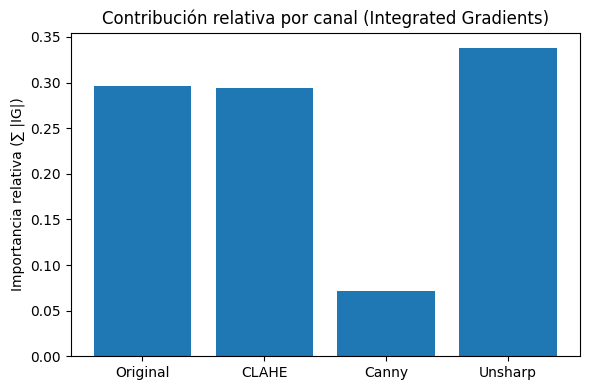
\includegraphics[width=0.45\textwidth]{images/ig_barchart.png}
    \caption{Contribució relativa per canal estimada a partir de les atribucions
    d’Integrated Gradients.}
    \label{fig:ig_barchart}
\end{figure}
La Figura~\ref{fig:ig_barchart} mostra la contribució relativa de cada canal
d’entrada, estimada mitjançant la suma del valor absolut de les atribucions
obtingudes amb Integrated Gradients. Aquesta representació permet comparar de
manera orientativa el pes relatiu de cada transformació d’entrada en la
predicció del model.

\subsection{Discussió dels resultats}

L’anàlisi qualitativa indica que el model no basa la seva decisió exclusivament
en un únic tipus de representació, sinó que combina informació procedent de
diversos canals. Els canals corresponents a la imatge original, CLAHE i Unsharp
presenten una contribució similar i dominant, fet que suggereix que el
classificador aprofita tant la informació radiològica original com el realce de
contrast i de detall fi per a la detecció de nòduls pulmonars. 

Per contra, el canal Canny mostra una contribució relativa clarament inferior.
Aquest comportament és coherent amb el fet que la detecció de contorns globals
del tòrax pot actuar com a informació auxiliar, però no resulta suficient per
si sola per a la identificació de lesions nodulars. Aquest resultat és
desitjable, ja que indica que el model no depèn principalment de contorns
anatòmics generals (costelles, diafragma o clavícules), sinó de patrons de
textura i detall més rellevants des del punt de vista clínic.

Cal remarcar que encara que els resultats son molt semblants a l'estudi d'ablacio fet  aquest anàlisi s’ha realitzat amb una finalitat
exploratòria i formativa, i que les conclusions extretes són de caràcter
qualitatiu degut al excas coneixament que tenen els autors en XAI. Tot i això, els resultats obtinguts suggereixen un comportament
coherent del model i proporcionen una primera evidència que el pipeline
multicanal utilitzat permet integrar diferents tipus d’informació de manera
complementària.
\newpage
\newpage

% ==================
% # DETECCIO
% ==================


\section{Inici de la fase de detecció de nòduls pulmonars}

Un cop completada i validada la fase de classificació, el següent pas natural del
treball és abordar la tasca de detecció de nòduls pulmonars. A diferència de la
classificació binària, la detecció requereix no només determinar la presència d’un
nòdul, sinó també localitzar-lo espacialment dins la radiografia mitjançant
\textit{bounding boxes}.

En aquesta fase s’aprofita íntegrament el pipeline de processament i entrenament
definit en les seccions anteriors, adaptant-lo a un escenari de detecció supervisada.
Els experiments realitzats exploren diferents estratègies de \textit{transfer learning},
arquitectures de detecció i representacions d’entrada, amb l’objectiu d’analitzar el
seu impacte en la capacitat de localització dels nòduls pulmonars.

\subsection{Anàlisi de la distribució espacial i del tamany dels nòduls pulmonars}

Abans d’abordar la tasca de detecció automàtica de nòduls pulmonars mitjançant models supervisats, s’ha dut a terme una anàlisi exploratòria del conjunt de dades amb l’objectiu de caracteritzar la distribució espacial dels nòduls i la seva variabilitat morfològica. Aquest estudi permet identificar possibles biaixos inherents al dataset i contextualitzar les dificultats associades a la detecció de lesions petites o de baix contrast.

La Figura~\ref{fig:spatial_distribution} mostra la distribució espacial bidimensional dels nòduls anotats, representada en coordenades normalitzades respecte a la mida de la imatge. S’observa clarament una distribució bimodal al llarg de l’eix horitzontal, corresponent als dos camps pulmonars, fet que reflecteix la coherència anatòmica del conjunt de dades. La regió central de la imatge, associada al mediastí, presenta una densitat molt baixa de nòduls, mentre que la major concentració es localitza dins del parènquima pulmonar.

\begin{figure}[H]
    \centering
    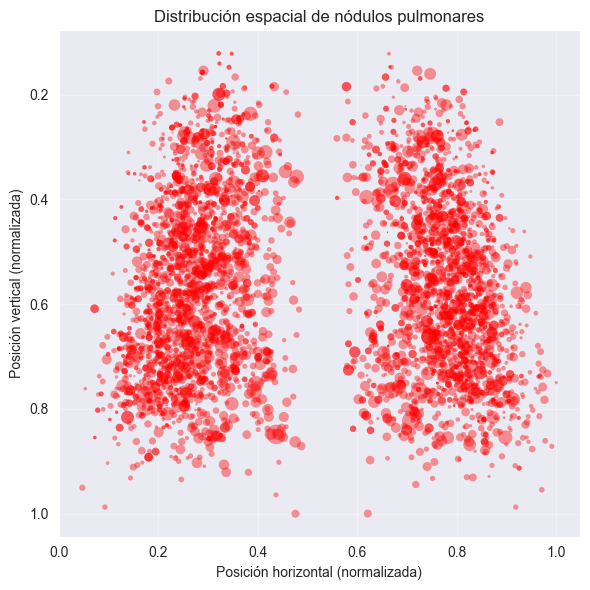
\includegraphics[width=0.99\linewidth]{images/distribucion_nodulos.png}
    \caption{Distribució espacial dels nòduls pulmonars en coordenades normalitzades.}
    \label{fig:spatial_distribution}
\end{figure}

Pel que fa a l’eix vertical, la distribució és més contínua, amb una lleugera concentració de nòduls en les regions mitjanes i inferiors dels pulmons. El tamany dels marcadors s’ha escalat proporcionalment a l’àrea del nòdul, fet que permet observar que els nòduls de major mida no es concentren en una regió específica, sinó que apareixen distribuïts de manera relativament homogènia dins de cada camp pulmonar.

La Figura~\ref{fig:size_distribution} presenta la distribució contínua del tamany dels nòduls, expressada en termes d’àrea en píxels quadrats i representada mitjançant una estimació de densitat amb escala logarítmica a l’eix horitzontal. La distribució obtinguda és clarament asimètrica, amb una cua llarga cap a valors elevats, indicant que la majoria de nòduls són de petit o mitjà tamany, mentre que les lesions de gran àrea són relativament infreqüents. Aquest comportament és típic de conjunts de dades clínics reals i representa un repte significatiu per als models de detecció, especialment pel que fa a la sensibilitat en nòduls petits.

\begin{figure}[H]
    \centering
    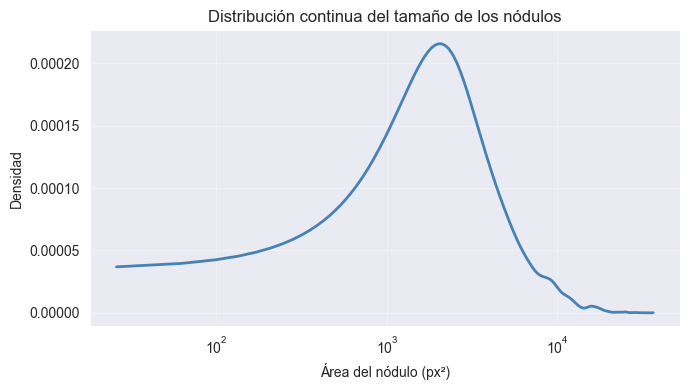
\includegraphics[width=0.99\linewidth]{images/distribucion_tamao_nodulo.png}
    \caption{Distribució contínua del tamany dels nòduls (àrea en px$^2$, escala logarítmica).}
    \label{fig:size_distribution}
\end{figure}

Finalment, la Figura~\ref{fig:size_vs_position} analitza la relació entre el tamany del nòdul i la seva posició radial respecte al centre de la imatge. Els resultats indiquen que no existeix una correlació forta entre ambdues variables: nòduls de diferents tamanys apareixen al llarg de tot el rang de distàncies radials. Tanmateix, s’observa una major densitat de nòduls a distàncies intermèdies, corresponents al parènquima pulmonar, mentre que les regions més centrals i perifèmodelriques presenten una menor concentració.

\begin{figure}[H]
    \centering
    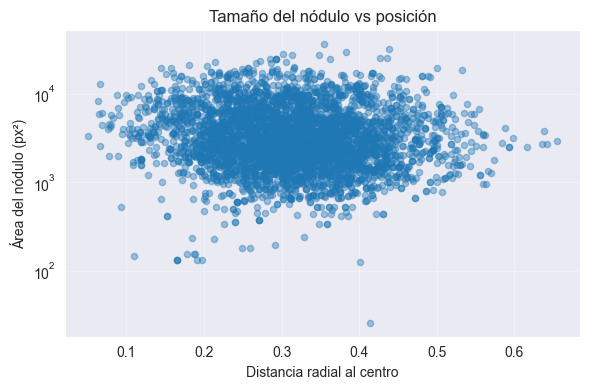
\includegraphics[width=0.99\linewidth]{images/tamano_nodulo_vs_posicion.png}
    \caption{Relació entre el tamany del nòdul i la distància radial al centre de la imatge.}
    \label{fig:size_vs_position}
\end{figure}

En conjunt, aquest anàlisi confirma que el conjunt de dades presenta una distribució espacial anatòmicament coherent i una elevada variabilitat en el tamany dels nòduls. Aquestes característiques justifiquen la necessitat d’emprar models de detecció robustos i multiescala, així com estratègies de preprocessament i transfer learning adaptades al domini radiològic.


\subsection*{Mètriques d’avaluació}

L’avaluació dels models de detecció desenvolupats en aquest treball es realitza
seguint un protocol alineat amb el repte \textit{NODE21}, dissenyat específicament
per a la detecció de nòduls pulmonars en radiografies de tòrax. Aquest enfocament
permet analitzar el rendiment dels models des d’una perspectiva clínicament
rellevant, tenint en compte no només la capacitat de detecció global, sinó també
el compromís entre sensibilitat i nombre de falsos positius per imatge.

En aquest context, les mètriques utilitzades van més enllà de les mesures
clàssiques de visió per computador i se centren en una anàlisi basada en la
corba \textit{Free-response Receiver Operating Characteristic} (FROC), que
caracteritza el comportament del detector en diferents règims d’operació.
A partir d’aquesta corba, s’avalua la sensibilitat del model a diversos nivells
de falsos positius per imatge, concretament a 0.25, 0.5, 1, 2, 4 i 8 FP/img.

Com a resum quantitatiu del rendiment global, s’utilitza el \textit{NODE21 score},
que agrega els valors de sensibilitat als punts de funcionament definits pel
repte. Addicionalment, es mesura el temps total d’inferència com a indicador de
la viabilitat computacional de cada model.

Aquest conjunt de mètriques proporciona una avaluació homogènia i reproduïble
de totes les configuracions estudiades, i permet comparar els models tant en
termes de rendiment global com segons criteris clínicament rellevants adaptats
a diferents escenaris d’ús.


% ==================
% # Faster R-CNN preentrenat en COCO
% ==================

\section{Model 1: Detecció amb Faster R-CNN preentrenat en COCO}

Com a primer enfocament per abordar la tasca de detecció de nòduls pulmonars, s’ha
optat per utilitzar una arquitectura de detecció consolidada i àmpliament utilitzada
en visió per computador: Faster R-CNN. L’objectiu d’aquest primer model és establir
una línia base funcional que permeti validar tot el pipeline de detecció abans
d’introduir modificacions específiques del domini mèdic o estratègies d’innovació.

El model utilitzat es basa en una arquitectura Faster R-CNN amb backbone ResNet50 i
Feature Pyramid Network (FPN), inicialment preentrenada sobre el conjunt de dades
COCO. L’ús de pesos preentrenats permet partir d’un conjunt de característiques
visuals generals apreses sobre un gran volum d’imatges, facilitant la convergència
del model en un escenari amb dades limitades.

En una primera fase, el model s’ha configurat mantenint congelat el backbone i
entrenant únicament la capçalera de detecció, adaptada al problema de NODE21. Aquesta
estratègia permet avaluar el comportament del detector utilitzant exclusivament les
representacions apreses durant el preentrenament sobre COCO.

A partir d’aquesta configuració inicial, es va adoptar una estratègia de
\textit{fine-tuning} parcial, en la qual es mantenen congelades les capes inicials del
backbone ResNet50 i es permet l’actualització dels pesos de les capes més profundes.
Aquesta decisió respon al fet que les capes inicials capturen característiques visuals
bàsiques i transferibles, mentre que les capes superiors poden adaptar-se a patrons
més específics de les radiografies de tòrax.

Finalment, la capçalera de classificació del model s’ha modificat per ajustar-se a un
escenari de dues classes: fons (\textit{background}) i nòdul pulmonar. Aquest model
constitueix el punt de partida per a la resta d’experiments de detecció presentats en
les seccions posteriors.




\begin{figure}[H]
    \centering
    \begin{subfigure}[H]{0.45\columnwidth}
        \centering
        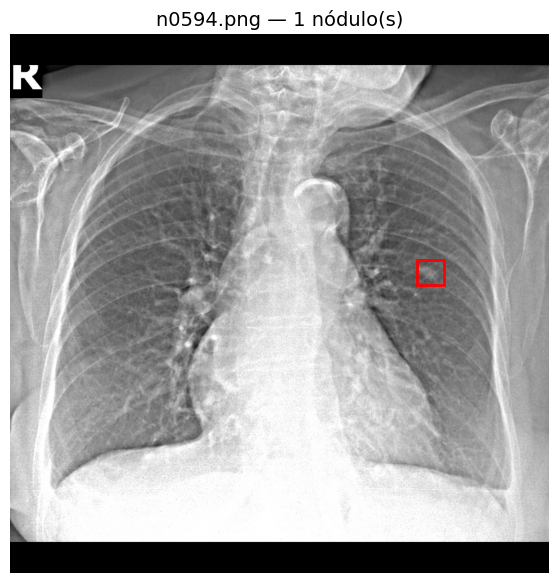
\includegraphics[width=\linewidth]{images/gt_example_frcnn.png}
        \caption{Anotació de referència (ground truth).}
    \end{subfigure}
    \hfill
    \begin{subfigure}[H]{0.45\columnwidth}
        \centering
        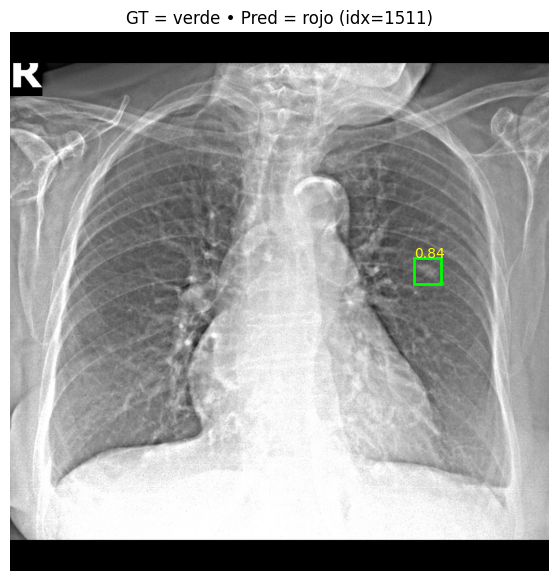
\includegraphics[width=\linewidth]{images/pred_example_frcnn.png}
        \caption{Predicció del model Faster R-CNN.}
    \end{subfigure}
    \caption{Comparació qualitativa entre les anotacions de referència i les deteccions
    generades pel Model 1 basat en Faster R-CNN preentrenat en COCO.}
    \label{fig:model1_detection}
\end{figure}


Com hem dit abans a més de la configuració amb backbone completament congelat, dins del mateix Model
1 s’ha explorat una estratègia de \textit{fine-tuning} parcial orientada a millorar
l’adaptació del detector al domini radiològic. En aquesta configuració, es mantenen
congelades les capes inicials del backbone ResNet50, mentre que es permet
l’actualització dels pesos corresponents al bloc \textit{layer4} i a la
\textit{Feature Pyramid Network} (FPN).

La decisió de descongelar exclusivament el bloc \textit{layer4} respon al fet que
aquestes capes capturen representacions d’alt nivell, potencialment més
específiques del domini, mentre que la FPN juga un paper crític en la detecció
d’objectes petits mitjançant la combinació d’informació multiescala. Aquesta
estratègia permet una adaptació controlada del model al domini de les
radiografies de tòrax, minimitzant alhora el risc de sobreajustament associat a un
\textit{fine-tuning} complet del backbone.



\subsection{Resultats quantitatius del Model 1}
Un cop entrenades les diferents variants del Model 1 basat en Faster R-CNN
preentrenat en COCO, s’ha procedit a l’avaluació quantitativa del seu rendiment
sobre el conjunt de validació de NODE21. Aquesta avaluació s’ha dut a terme
utilitzant el mateix pipeline d’inferència i les mateixes mètriques emprades de
manera sistemàtica a la resta d’experiments, garantint així la comparabilitat
directa dels resultats.

En aquesta secció es consideren exclusivament configuracions \textbf{monocanal},
tant amb backbone completament congelat com amb \textit{fine-tuning} parcial
mitjançant la descongelació del bloc \textit{layer4} i de la FPN. Aquesta decisió
permet analitzar de manera aïllada l’impacte de l’adaptació del backbone al domini
radiològic, sense introduir altres factors de variabilitat.


L’avaluació s’ha realitzat mitjançant mètriques específiques de detecció,
incloent-hi la sensibilitat, el nombre mitjà de falsos positius per imatge i el
valor mitjà de la intersecció sobre unió (IoU) per a les deteccions correctes, així
com les mètriques oficials del repte NODE21 quan escau. Aquests indicadors són
especialment rellevants en un context clínic, on la capacitat de detectar nòduls
petits amb un nombre controlat de falsos positius és crítica.

\begin{figure}[H]
    \centering
    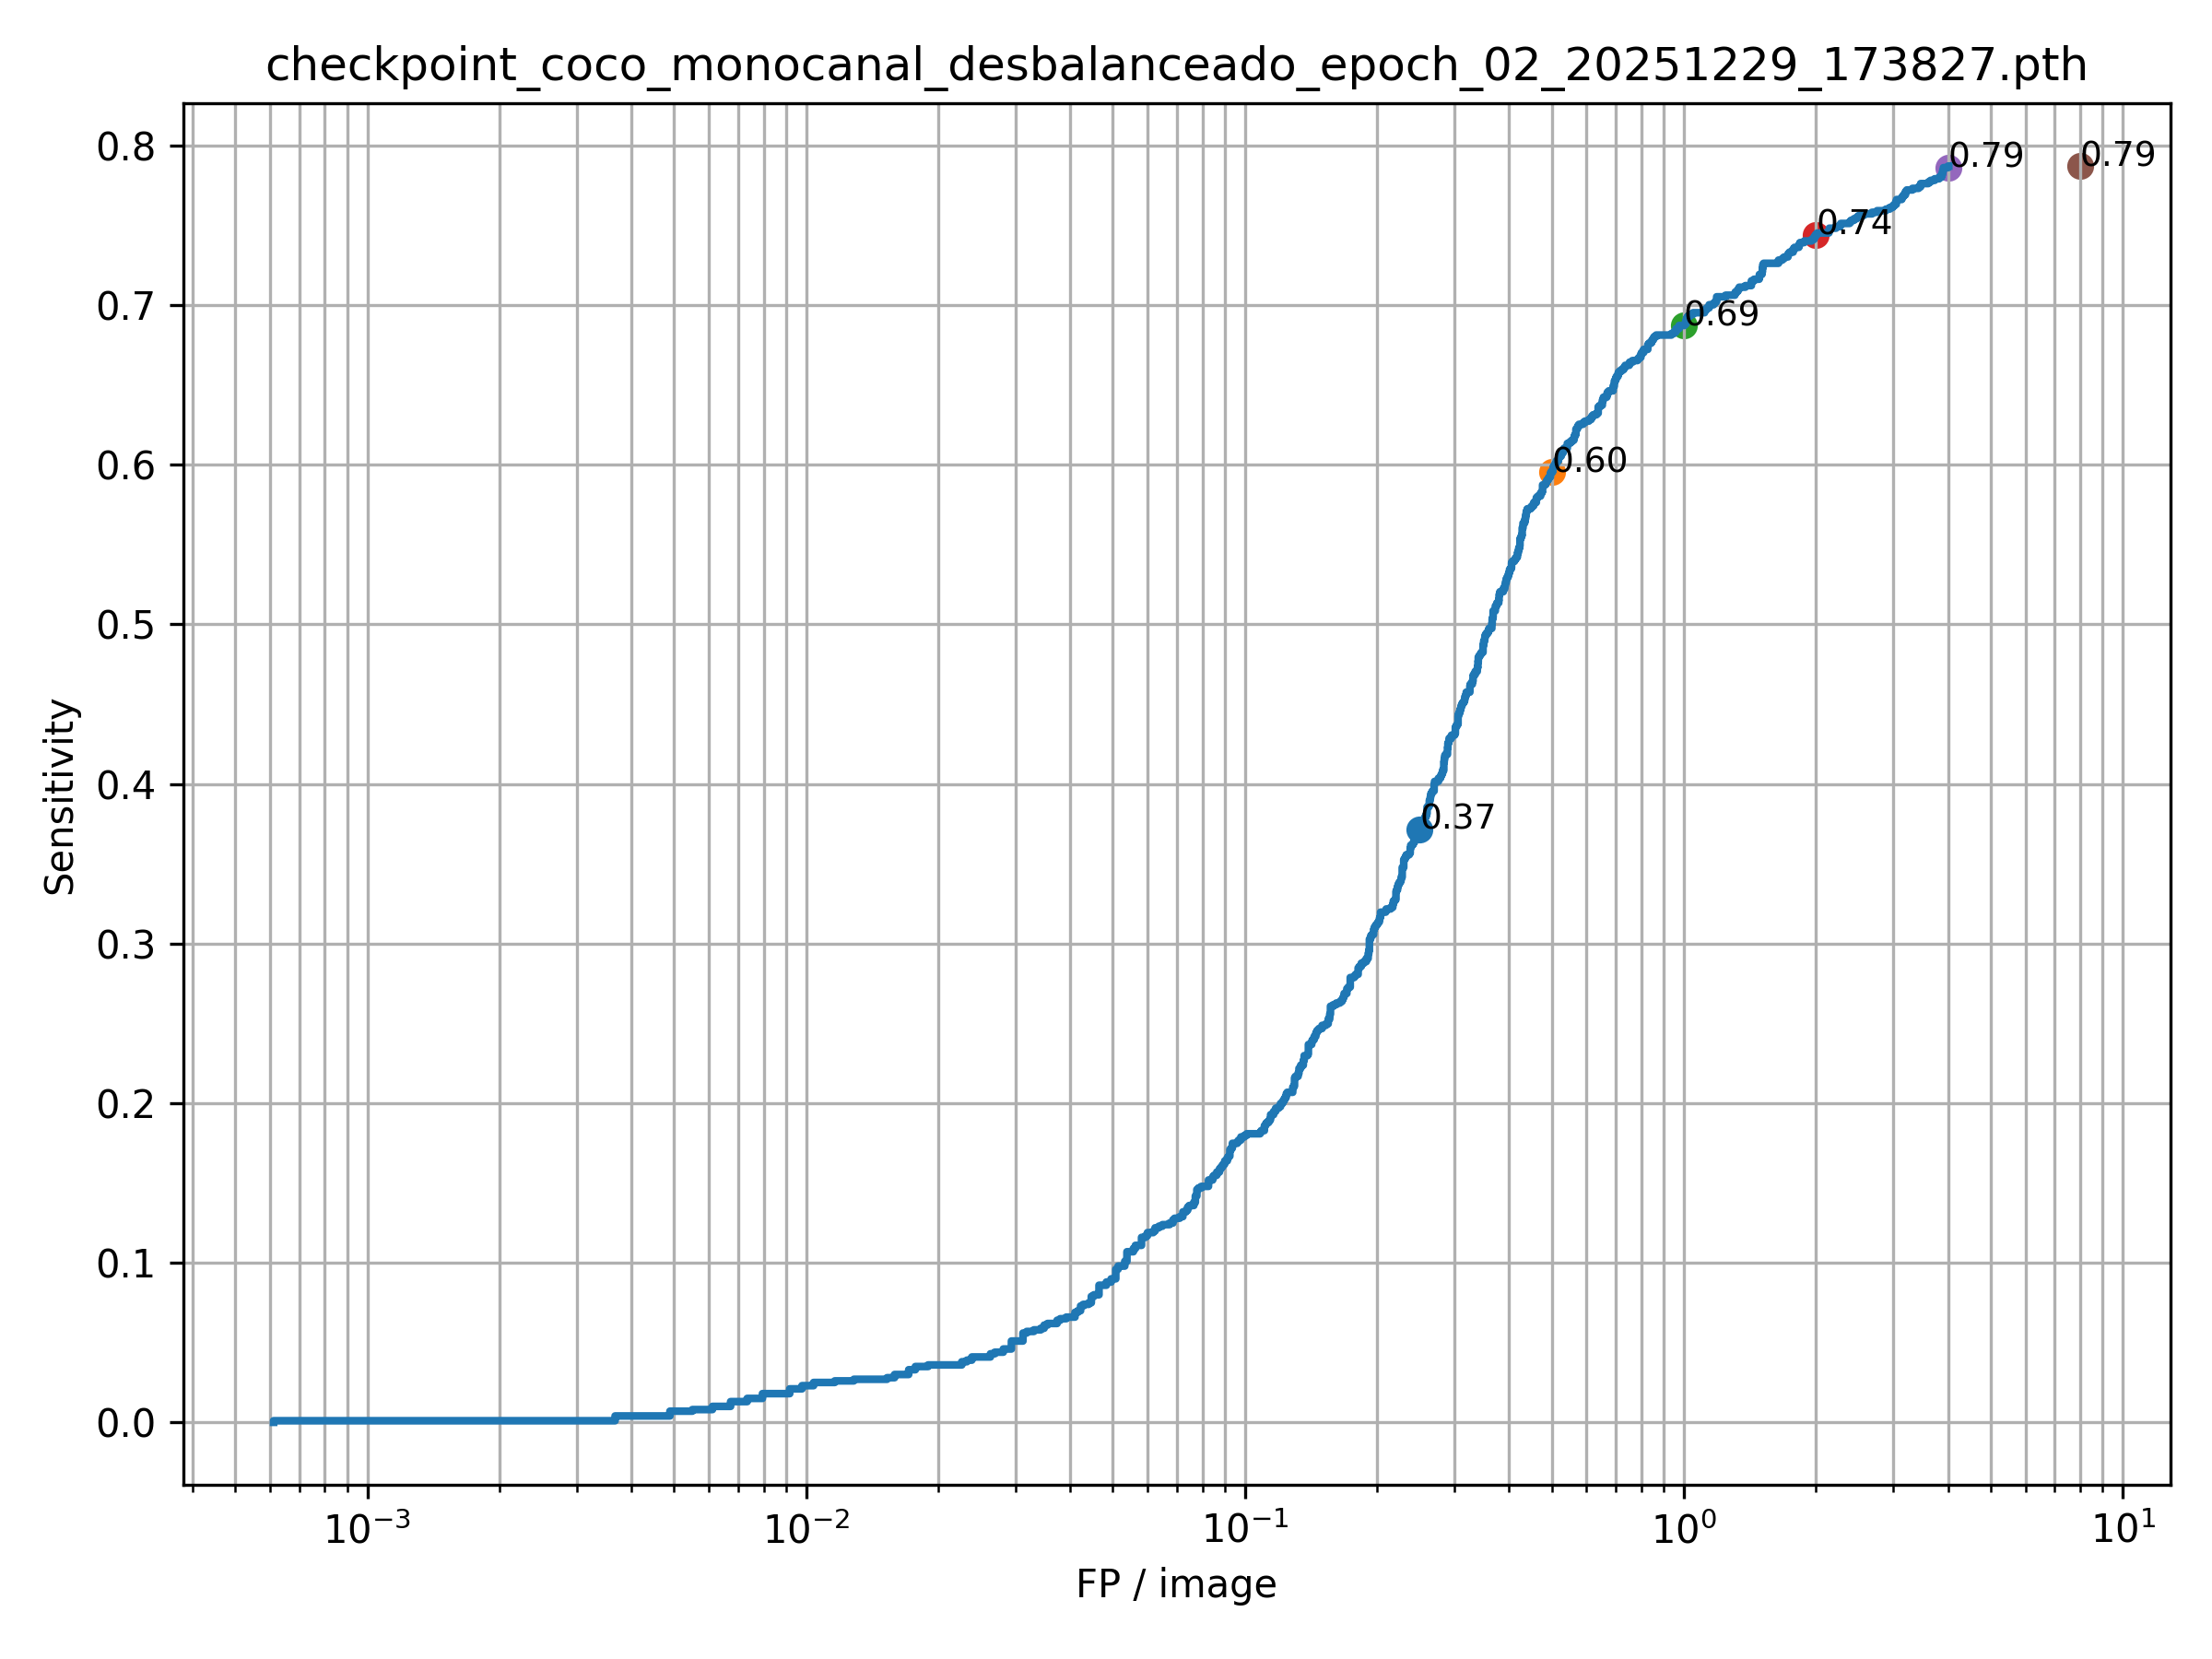
\includegraphics[width=0.8\columnwidth]{images/checkpoint_coco_monocanal_desbalanceado_epoch_02_20251229_173827_froc.png}
    \caption{Corba FROC del millor checkpoint del Model 1 (Faster R-CNN preentrenat en COCO, configuració monocanal i dataset no balancejat). 
    Els punts ressaltats indiquen els valors de sensibilitat assolits als nivells de falsos positius per imatge utilitzats en l’avaluació oficial del repte NODE21.}
    \label{fig:model1_coco_froc}
\end{figure}

\begin{figure}[H]
    \centering
    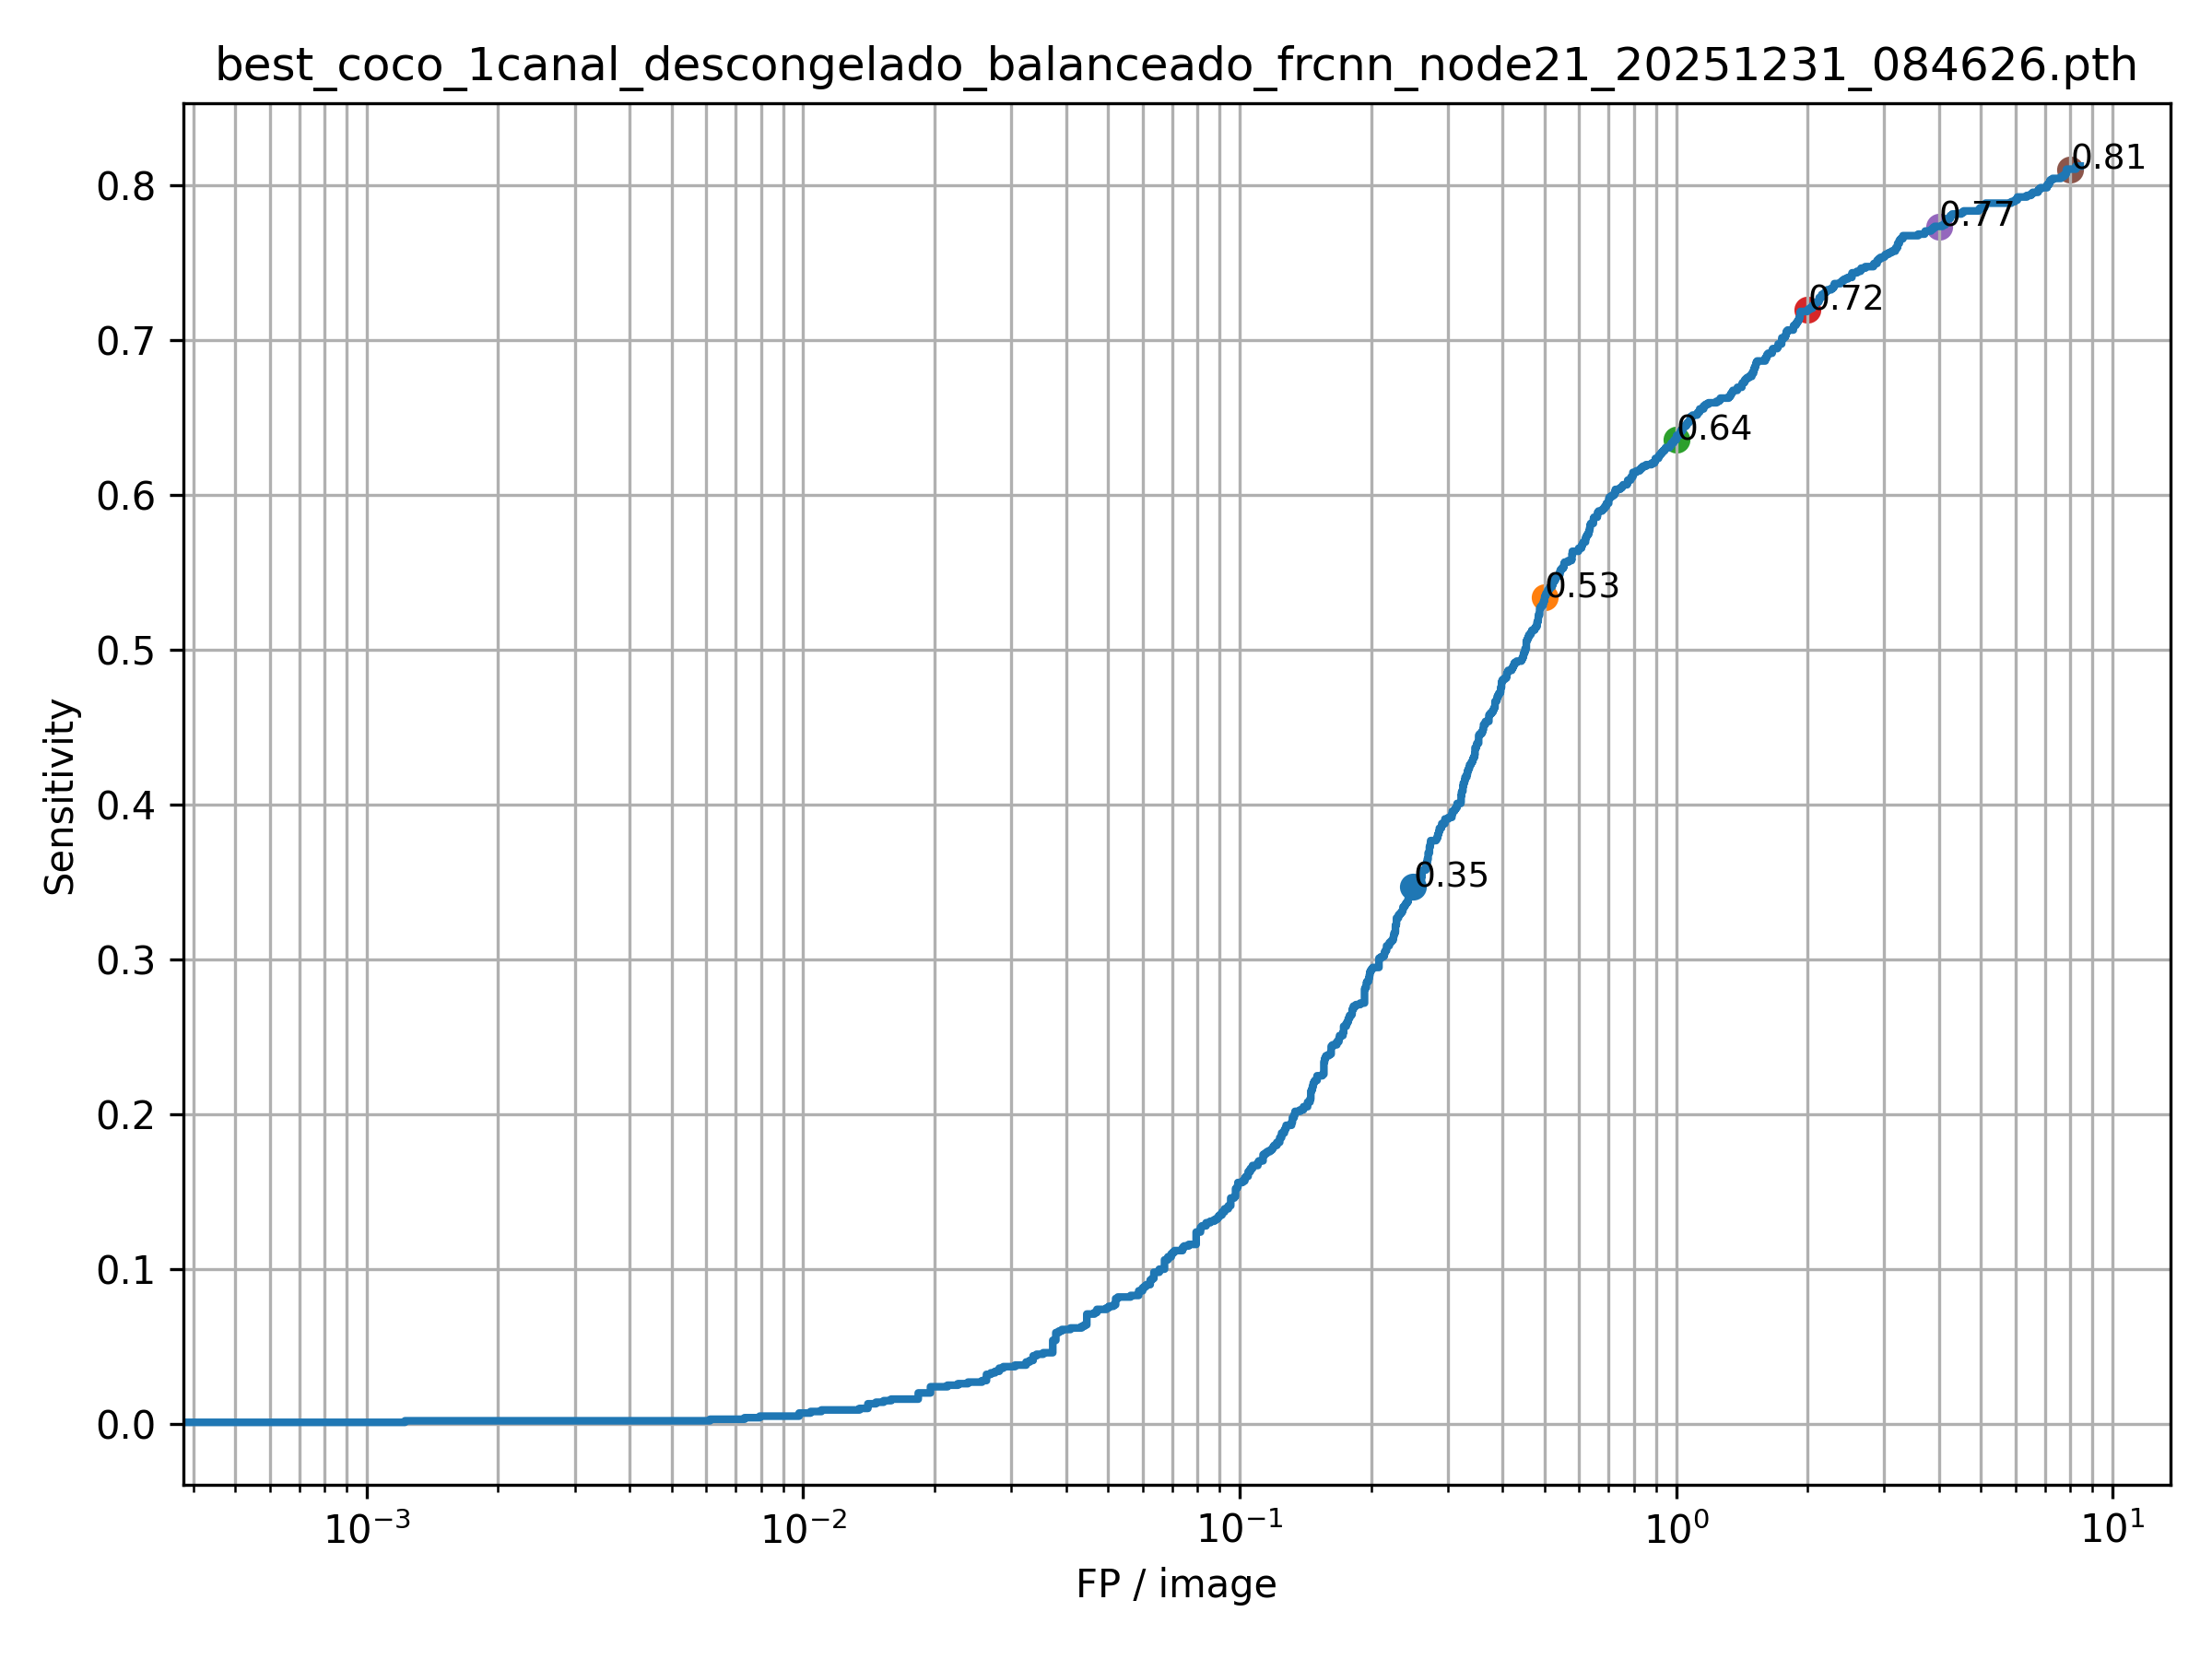
\includegraphics[width=0.8\columnwidth]{images/best_coco_1canal_descongelado_balanceado_frcnn_node21_20251231_084626_froc.png}
    \caption{Corba FROC del millor checkpoint del Model COCO amb \textit{fine-tuning} parcial
    (descongelació del bloc \textit{layer4} del backbone i de la FPN) i entrada monocanal.
    Els punts ressaltats indiquen els valors de sensibilitat als nivells de falsos positius
    per imatge utilitzats en l’avaluació NODE21.}
    \label{fig:model1_coco_unfrozen_froc}
\end{figure}



\subsection{Avaluació quantitativa del Model 1}

El model amb pessos congelats assoleix un NODE21 score de 0.662, amb una sensibilitat del 0.372 a
0.25 falsos positius per imatge, incrementant-se progressivament fins a valors
propers al 0.79 a partir de 4 falsos positius per imatge. Aquest comportament
reflecteix una capacitat raonable de detecció en règims de baixa taxa de falsos
positius, tot i les limitacions inherents a l’ús de representacions visuals
generals apreses sobre imatges naturals.

Els valors puntuals de sensibilitat obtinguts per aquest model són:

\begin{table}[H]
\centering
\footnotesize
\caption{Sensibilitat del Model 1 (Faster R-CNN preentrenat en COCO amb backbone congelat) a diferents nivells de falsos positius per imatge}
\label{tab:model1_coco_frozen_sensitivity}
\setlength{\tabcolsep}{6pt}
\begin{tabular}{cc}
\toprule
\textbf{FP per imatge} & \textbf{Sensibilitat} \\
\midrule
0.25 & 0.372 \\
0.5  & 0.595 \\
1    & 0.687 \\
2    & 0.744 \\
4    & 0.786 \\
8    & 0.787 \\
\bottomrule
\end{tabular}
\end{table}



A més de la configuració base amb backbone completament congelat, s’ha avaluat una
variant amb \textit{fine-tuning} parcial en la qual es permet l’actualització dels pesos
del bloc \textit{layer4} del ResNet50 i de la \textit{Feature Pyramid Network} (FPN),
mantenint congelades la resta de capes. Aquesta estratègia pretén afavorir l’adaptació
al domini radiològic sense fer un reentrenament complet del backbone.

Els valors puntuals de sensibilitat obtinguts per aquesta configuració són:

\begin{table}[H]
\centering
\footnotesize
\caption{Sensibilitat del Model 1 (Faster R-CNN preentrenat en COCO amb \textit{fine-tuning} parcial de \textit{layer4} i FPN) a diferents nivells de falsos positius per imatge}
\label{tab:model1_coco_unfrozen_sensitivity}
\setlength{\tabcolsep}{6pt}
\begin{tabular}{cc}
\toprule
\textbf{FP per imatge} & \textbf{Sensibilitat} \\
\midrule
0.25 & 0.350 \\
0.5  & 0.530 \\
1    & 0.640 \\
2    & 0.720 \\
4    & 0.770 \\
8    & 0.810 \\
\bottomrule
\end{tabular}
\end{table}



La Figura~\ref{fig:model1_coco_unfrozen_froc} mostra la corba FROC del millor checkpoint
d’aquesta configuració. En aquest cas, el rendiment global obtingut és
\textbf{moderat}, amb un \textbf{NODE21 score de 0.63} (segons l’avaluació del pipeline
implementat en aquest treball) i una sensibilitat que augmenta de manera
progressiva a mesura que es relaxa el nombre de falsos positius per imatge.


Comparant amb la configuració COCO amb backbone congelat, els resultats indiquen que el
\textit{fine-tuning} parcial no garanteix una millora sistemàtica del NODE21 score. Aquest
comportament suggereix que, tot i que la descongelació de \textit{layer4} i FPN pot ajudar
a reajustar representacions multiescala, la limitació principal continua sent el desajust
entre el domini del preentrenament (imatges naturals) i el domini radiològic objectiu.
Aquesta observació reforça la necessitat d’explorar pesos preentrenats en conjunts de dades
radiològiques específiques, com VinDr-CXR, on els resultats sí mostren un salt substancial
de rendiment.


En conjunt, aquests resultats confirmen que el model Faster R-CNN preentrenat en
COCO constitueix una línia base funcional i estable, capaç de localitzar nòduls
pulmonars amb un rendiment moderat. Tanmateix, la sensibilitat assolida en règims
de baixa taxa de falsos positius és limitada, fet que suggereix que les
característiques apreses sobre imatges naturals no són suficients per capturar
plenament els patrons radiològics associats als nòduls pulmonars.

Aquesta observació justifica l’exploració de pesos preentrenats en dominis
radiològics específics, com VinDr-CXR, així com l’ús de representacions d’entrada
enriquides, que es presenten en els models posteriors.






% ==================
% # Faster R-CNN preentrenat amb pesos VinDr-CXR
% ==================

\section{Model 2: Detecció amb Faster R-CNN preentrenat amb pesos VinDr-CXR}

En una fase posterior del treball, s’ha optat per reproduir i analitzar l’enfocament
utilitzat pel model guanyador del repte NODE21, amb l’objectiu d’avaluar fins a quin punt
aquesta estratègia pot ser replicada i adaptada al conjunt de dades emprat en aquest estudi.

A partir d’una revisió detallada de l’article associat al repte NODE21, es va identificar
que el millor rendiment no s’assolia mitjançant un model inicialitzat amb pesos d’ImageNet
o COCO, sinó amb un model Faster R-CNN amb backbone ResNet50-FPN inicialitzat amb
pesos preentrenats sobre el conjunt de dades VinDr-CXR. Aquest fet representa una diferència
clau respecte a enfocaments més genèrics, ja que VinDr-CXR és un dataset específic de
radiografies de tòrax amb anotacions locals realitzades per múltiples radiòlegs.

El conjunt VinDr-CXR inclou més de 18.000 radiografies posteroanteriors de tòrax amb
anotacions de fins a 22 troballes toràciques, entre les quals s’inclou explícitament la
categoria \textit{Nodule/Mass}. Aquesta coincidència semàntica i visual amb la tasca de
detecció de nòduls pulmonars abordada en NODE21 el converteix en un domini d’entrenament
altament rellevant per a la transferència de coneixement.

A partir d’aquesta observació, es va iniciar un contacte directe amb els
autors amb l’objectiu de sol·licitar els pesos exactes utilitzats en els experiments del repte
NODE21. Com a resultat d’aquest intercanvi, els autors van facilitar els pesos del model
entrenat sobre VinDr-CXR, fet que ha permès dur a terme una reproducció inicial molt semblant a la de
l’estratègia guanyadora.

Aquest procés , que combina revisió bibliogràfica, anàlisi del model descrit a la
literatura i comunicació directa amb els investigadors responsables del dataset, posa
de manifest una voluntat explícita per part nostre de rigor científic i reproductibilitat, alineada amb
les bones pràctiques en recerca en aprenentatge profund aplicat a imatge mèdica.

Des del punt de vista tècnic, el model es construeix inicialitzant una arquitectura
Faster R-CNN amb ResNet50-FPN sense pesos per defecte, sobre la qual es carreguen
manualment els pesos preentrenats amb VinDr-CXR. Atès que el model original havia estat
entrenat per a un nombre superior de classes, s’elimina explícitament la capçalera de
classificació i regressió de caixes abans de redefinir-la per al cas binari de NODE21
(fons i nòdul pulmonar).

Seguint l’estratègia descrita pels autors del model guanyador, s’ha optat per congelar
inicialment tot el backbone convolucional i descongelar únicament les capes més profundes
(\textit{layer4}) juntament amb la Feature Pyramid Network (FPN). Aquest plantejament
permet preservar el coneixement adquirit durant l’entrenament sobre VinDr-CXR, alhora
que facilita una adaptació progressiva al domini específic de NODE21 mitjançant
\textit{fine-tuning} controlat.

Finalment, es redefineix la capçalera de detecció per ajustar-la a la tasca binària
plantejada i el model es prepara per al seu entrenament. Aquest segon model constitueix
una extensió directa del model base preentrenat en COCO i estableix una referència
fonamental per analitzar l’impacte d’utilitzar pesos preentrenats en un domini mèdic
altament relacionat amb la tasca objectiu.


\subsection{Resultats quantitatius del Model basat en VinDr-CXR}

Un cop entrenat el model Faster R-CNN inicialitzat amb pesos preentrenats en
VinDr-CXR, s’ha procedit a l’avaluació quantitativa del seu rendiment sobre el
conjunt de validació de NODE21 utilitzant el mateix pipeline d’inferència i les
mateixes mètriques emprades en la resta d’experiments. Aquest plantejament permet
una comparació directa i justa amb el model base preentrenat en COCO.

A diferència del cas COCO, en aquesta secció es consideren tant configuracions
\textbf{monocanal} com \textbf{multicanal} (tres canals), atès que ambdues han
mostrat un comportament consistent i un rendiment elevat. Els checkpoints
seleccionats corresponen als millors resultats obtinguts segons el NODE21 score,
evitant l’anàlisi de variabilitat entre èpoques que no aporta informació
addicional rellevant.


\begin{figure}[H]
    \centering
    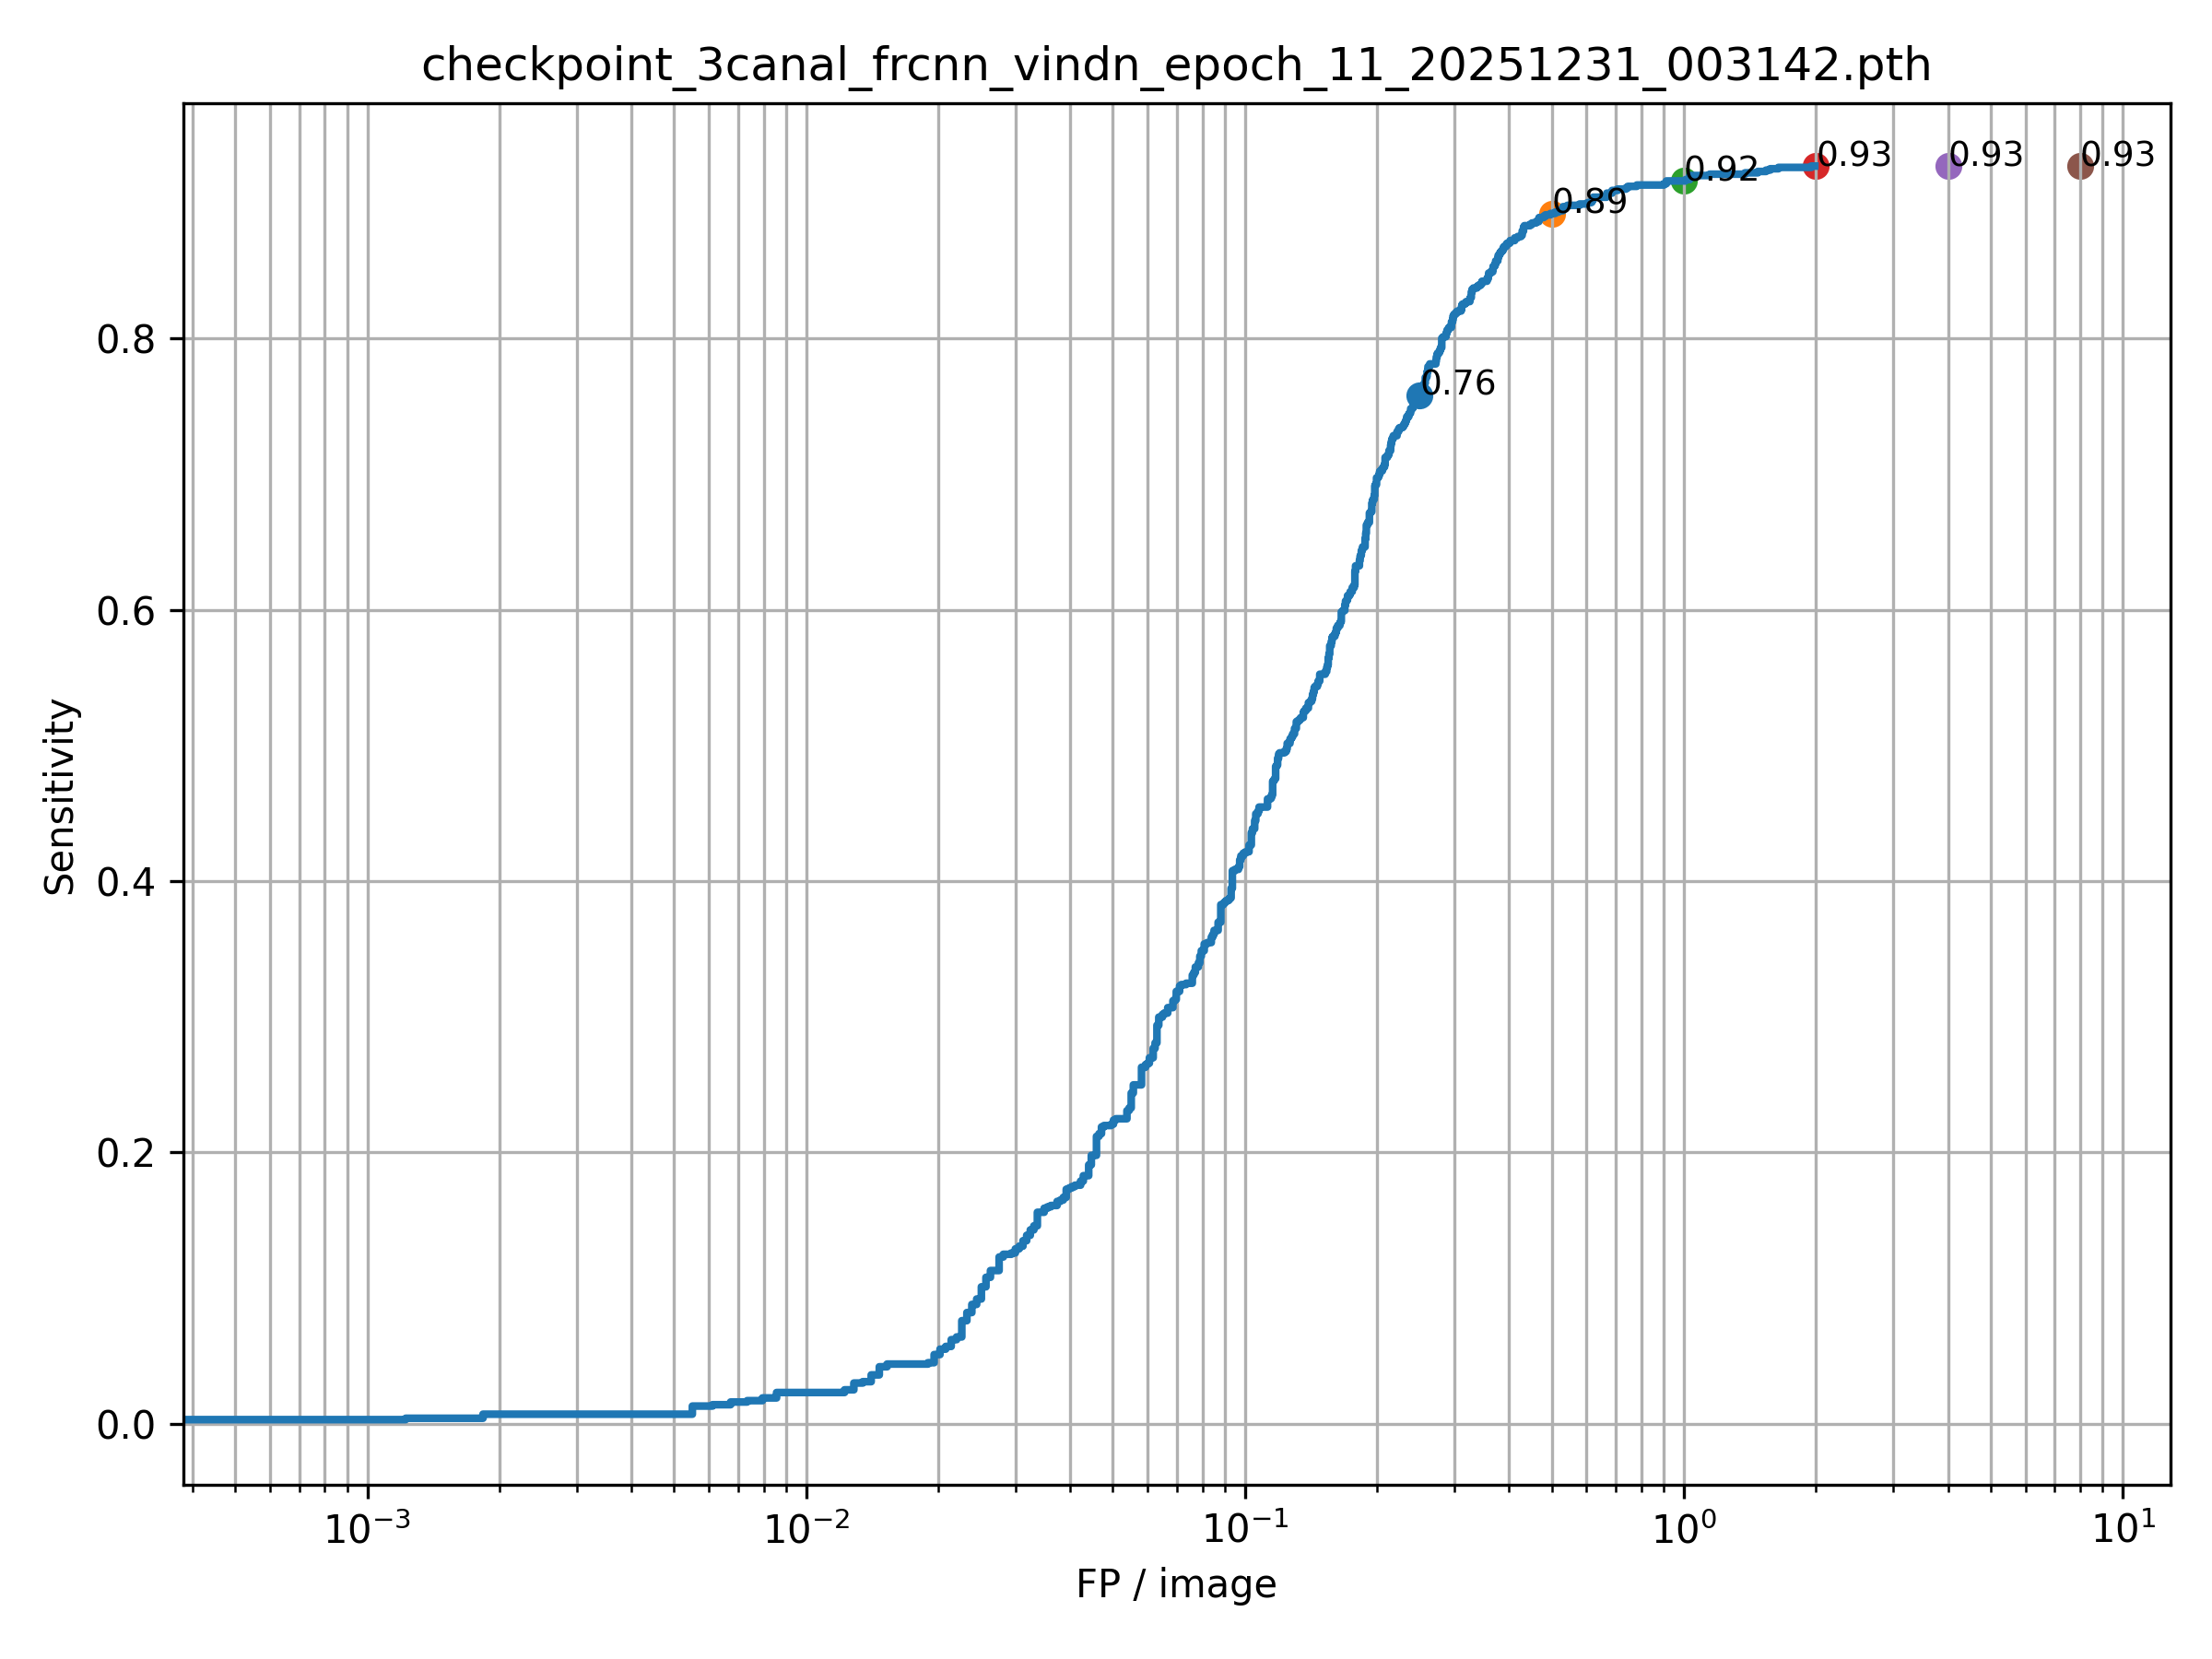
\includegraphics[width=0.8\columnwidth]{images/checkpoint_3canal_frcnn_vindn_epoch_11_20251231_003142_froc.png}
    \caption{Corba FROC del millor checkpoint del model Faster R-CNN preentrenat en
    VinDr-CXR amb representació multicanal (tres canals). Els punts ressaltats
    indiquen els valors de sensibilitat obtinguts als nivells de falsos positius per
    imatge utilitzats en l’avaluació oficial del repte NODE21.}
    \label{fig:model_vindr_froc}
\end{figure}


El millor checkpoint del model preentrenat en VinDr-CXR assoleix un
\textbf{NODE21 score de 0.89}, amb una \textbf{sensibilitat del 0.76} a
\textbf{0.25 falsos positius per imatge}, que s’incrementa de manera
progressiva fins a \textbf{valors superiors al 0.92} a partir de
\textbf{1 fals positiu per imatge}. Aquest comportament representa una
\textbf{millora substancial} respecte al model preentrenat en COCO en
\textbf{tots els règims d’operació analitzats}.

Els valors puntuals de sensibilitat obtinguts pel millor model multicanal són:


\begin{table}[H]
\centering
\footnotesize
\caption{Sensibilitat del model Faster R-CNN preentrenat en VinDr-CXR a diferents nivells de falsos positius per imatge}
\label{tab:sensitivity_vindr}
\setlength{\tabcolsep}{6pt}
\begin{tabular}{cc}
\toprule
\textbf{FP per imatge} & \textbf{Sensibilitat} \\
\midrule
0.25 & 0.758 \\
0.5  & 0.892 \\
1    & 0.916 \\
2    & 0.927 \\
4    & 0.927 \\
8    & 0.927 \\
\bottomrule
\end{tabular}
\end{table}


La comparació entre configuracions monocanal i multicanal en el cas del
preentrenament VinDr-CXR mostra que l’ús de tres canals d’entrada tendeix a oferir
un rendiment lleugerament superior en termes de NODE21 score i sensibilitat
global. Tanmateix, la diferència observada és reduïda i no es manifesta de manera
uniforme en tots els punts de la corba FROC.

Aquest resultat suggereix que, un cop el backbone ha estat preentrenat en un
domini radiològic específic, la representació monocanal ja captura gran part de
la informació rellevant per a la detecció de nòduls pulmonars, i que l’aportació
addicional dels canals CLAHE i \textit{unsharp masking} té un impacte marginal.


En conjunt, aquests resultats posen de manifest que el factor determinant del
rendiment del detector no és tant la representació multicanal de l’entrada com
l’alineació entre el domini del preentrenament i la tasca clínica objectiu. El
preentrenament en VinDr-CXR permet aprendre característiques radiològiques
específiques que es transfereixen de manera molt efectiva a la detecció de
nòduls pulmonars en NODE21.

Tot i que els valors assolits són comparables o superiors als reportats en el
repte NODE21, no és possible establir una comparació directa amb els resultats
oficials del concurs, ja que no es disposa d’informació sobre el subconjunt
exacte de radiografies utilitzat durant l’avaluació original.




% ==================
% # Faster R-CNN preentrenat amb pesos VinDr-CXR i COCO
% # Anàlisi monocanal vs representació multicanal
% ==================

\subsection{Anàlisi de la representació d’entrada: monocanal vs multicanal}

Des del disseny inicial dels experiments de detecció, els models Faster R-CNN
s’han entrenat de manera sistemàtica utilitzant tant una representació
\textbf{monocanal} com una representació \textbf{multicanal} de les imatges
d’entrada. Aquesta decisió permet analitzar de forma controlada l’impacte del
nombre de canals d’entrada en el rendiment del detector, sense introduir aquest
factor com una extensió posterior als entrenaments ja finalitzats.

En concret, per a ambdues configuracions base de detecció —Faster R-CNN
inicialitzat amb pesos COCO i Faster R-CNN inicialitzat amb pesos VinDr-CXR—,
s’han dut a terme entrenaments paral·lels emprant tant la imatge original en
escala de grisos com una representació multicanal basada en tres canals.

L’objectiu principal d’aquesta secció no és introduir una nova
arquitectura, sinó analitzar fins a quin punt el nombre de canals d’entrada
influeix en el rendiment del detector, mantenint constants la resta de factors.

La representació multicanal utilitzada es fonamenta en els resultats obtinguts
durant la fase de classificació, on es va observar que la combinació de diferents
transformacions d’intensitat podia aportar informació complementària. En
particular, s’han considerat tres canals: la imatge original normalitzada, una
versió amb realç de contrast mitjançant CLAHE i una versió amb realç de vores
basada en \textit{unsharp masking}. Aquests canals s’apilen per formar una entrada
compatible amb l’arquitectura Faster R-CNN, sense modificar la resta del pipeline
de detecció.



\begin{figure}[H]
    \centering
    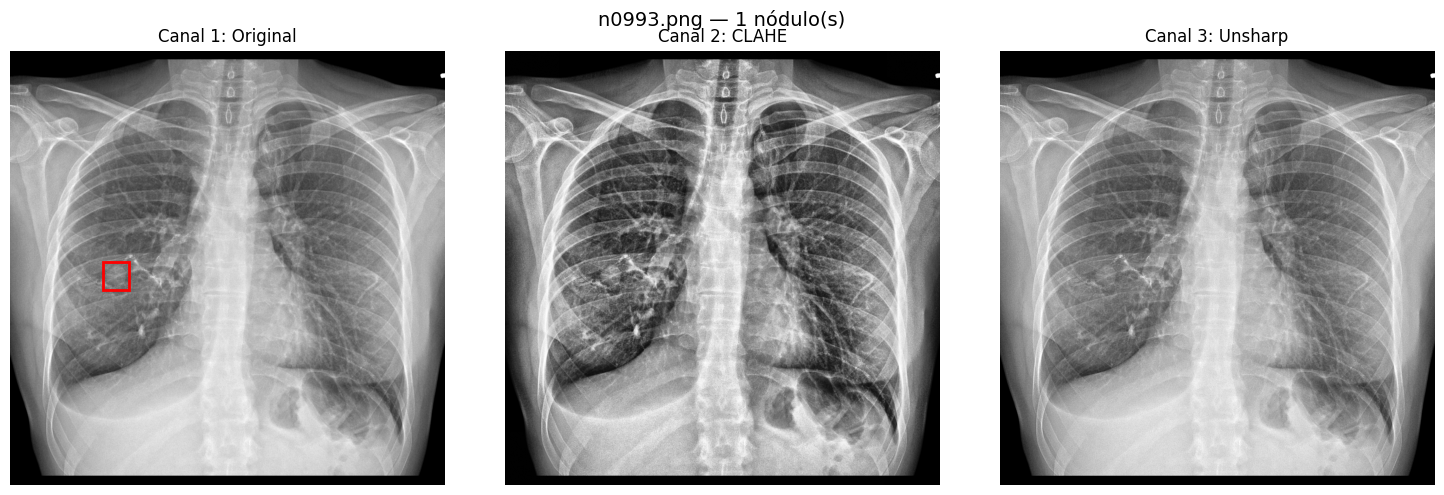
\includegraphics[width=0.8\columnwidth]{images/3_imagenes_gt.png}
    \caption{Visualització conjunta dels tres canals utilitzats com a entrada del
    model: imatge original, CLAHE i \textit{unsharp masking}. El \textit{bounding box}
    en color vermell indica l’anotació de referència (\textit{ground truth}) del
    nòdul pulmonar.}
    \label{fig:multichannel_gt}
\end{figure}

Des del punt de vista metodològic, tots els altres components del sistema es
mantenen estrictament idèntics als experiments anteriors. No es modifiquen ni les
anotacions ni els \textit{bounding boxes}, ni l’arquitectura del model, ni
l’estratègia d’entrenament o els criteris d’aturada primerenca. D’aquesta manera,
qualsevol diferència observada en el rendiment pot atribuir-se exclusivament a la
representació d’entrada utilitzada.

\begin{figure}[H]
    \centering
    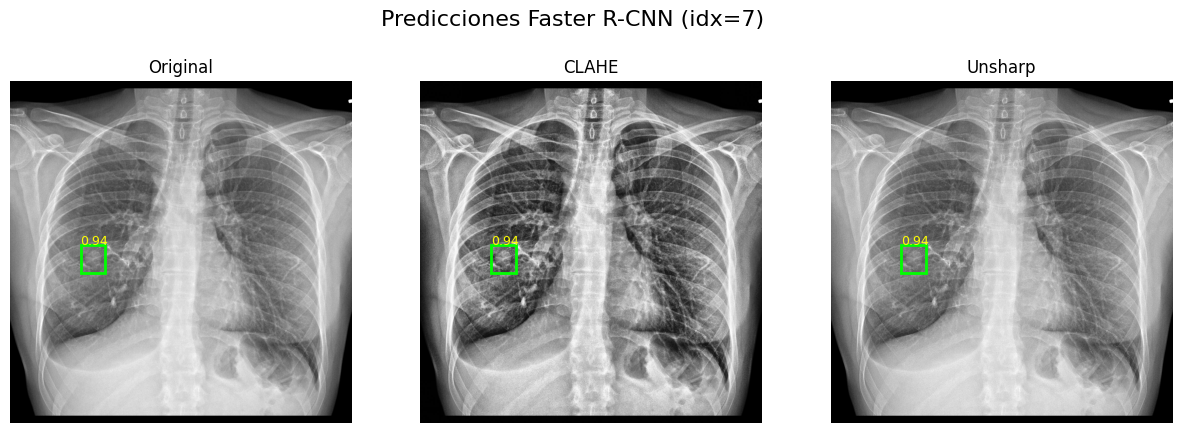
\includegraphics[width=0.8\columnwidth]{images/3_imagenes_pred.png}
    \caption{Resultat de la detecció automàtica del model Faster R-CNN entrenat amb
    representació multicanal. El \textit{bounding box} en color verd llima (lime)
    correspon a la predicció del model sobre la mateixa imatge mostrada a la
    Figura~\ref{fig:multichannel_gt}.}
    \label{fig:prediction_lime}
\end{figure}

L’anàlisi comparativa de les mètriques obtingudes amb pesos COCO mostra que la
utilització de tres canals d’entrada no comporta una millora sistemàtica respecte
a la configuració monocanal. Tot i que en alguns checkpoints s’observa un lleuger
increment de la sensibilitat en règims de falsos positius mitjans o elevats, aquest
guany no es reflecteix de manera consistent en el NODE21 score global. En règims
de baixa taxa de falsos positius, especialment rellevants en un context clínic, la
configuració monocanal tendeix a presentar un comportament més estable.

Aquest resultat suggereix que, en el cas del preentrenament en COCO, el backbone
no és capaç d’explotar plenament la informació addicional aportada pels canals
derivats, ja que aquestes transformacions no formen part del domini visual original
del preentrenament, basat en imatges naturals.

\begin{figure}[H]
    \centering
    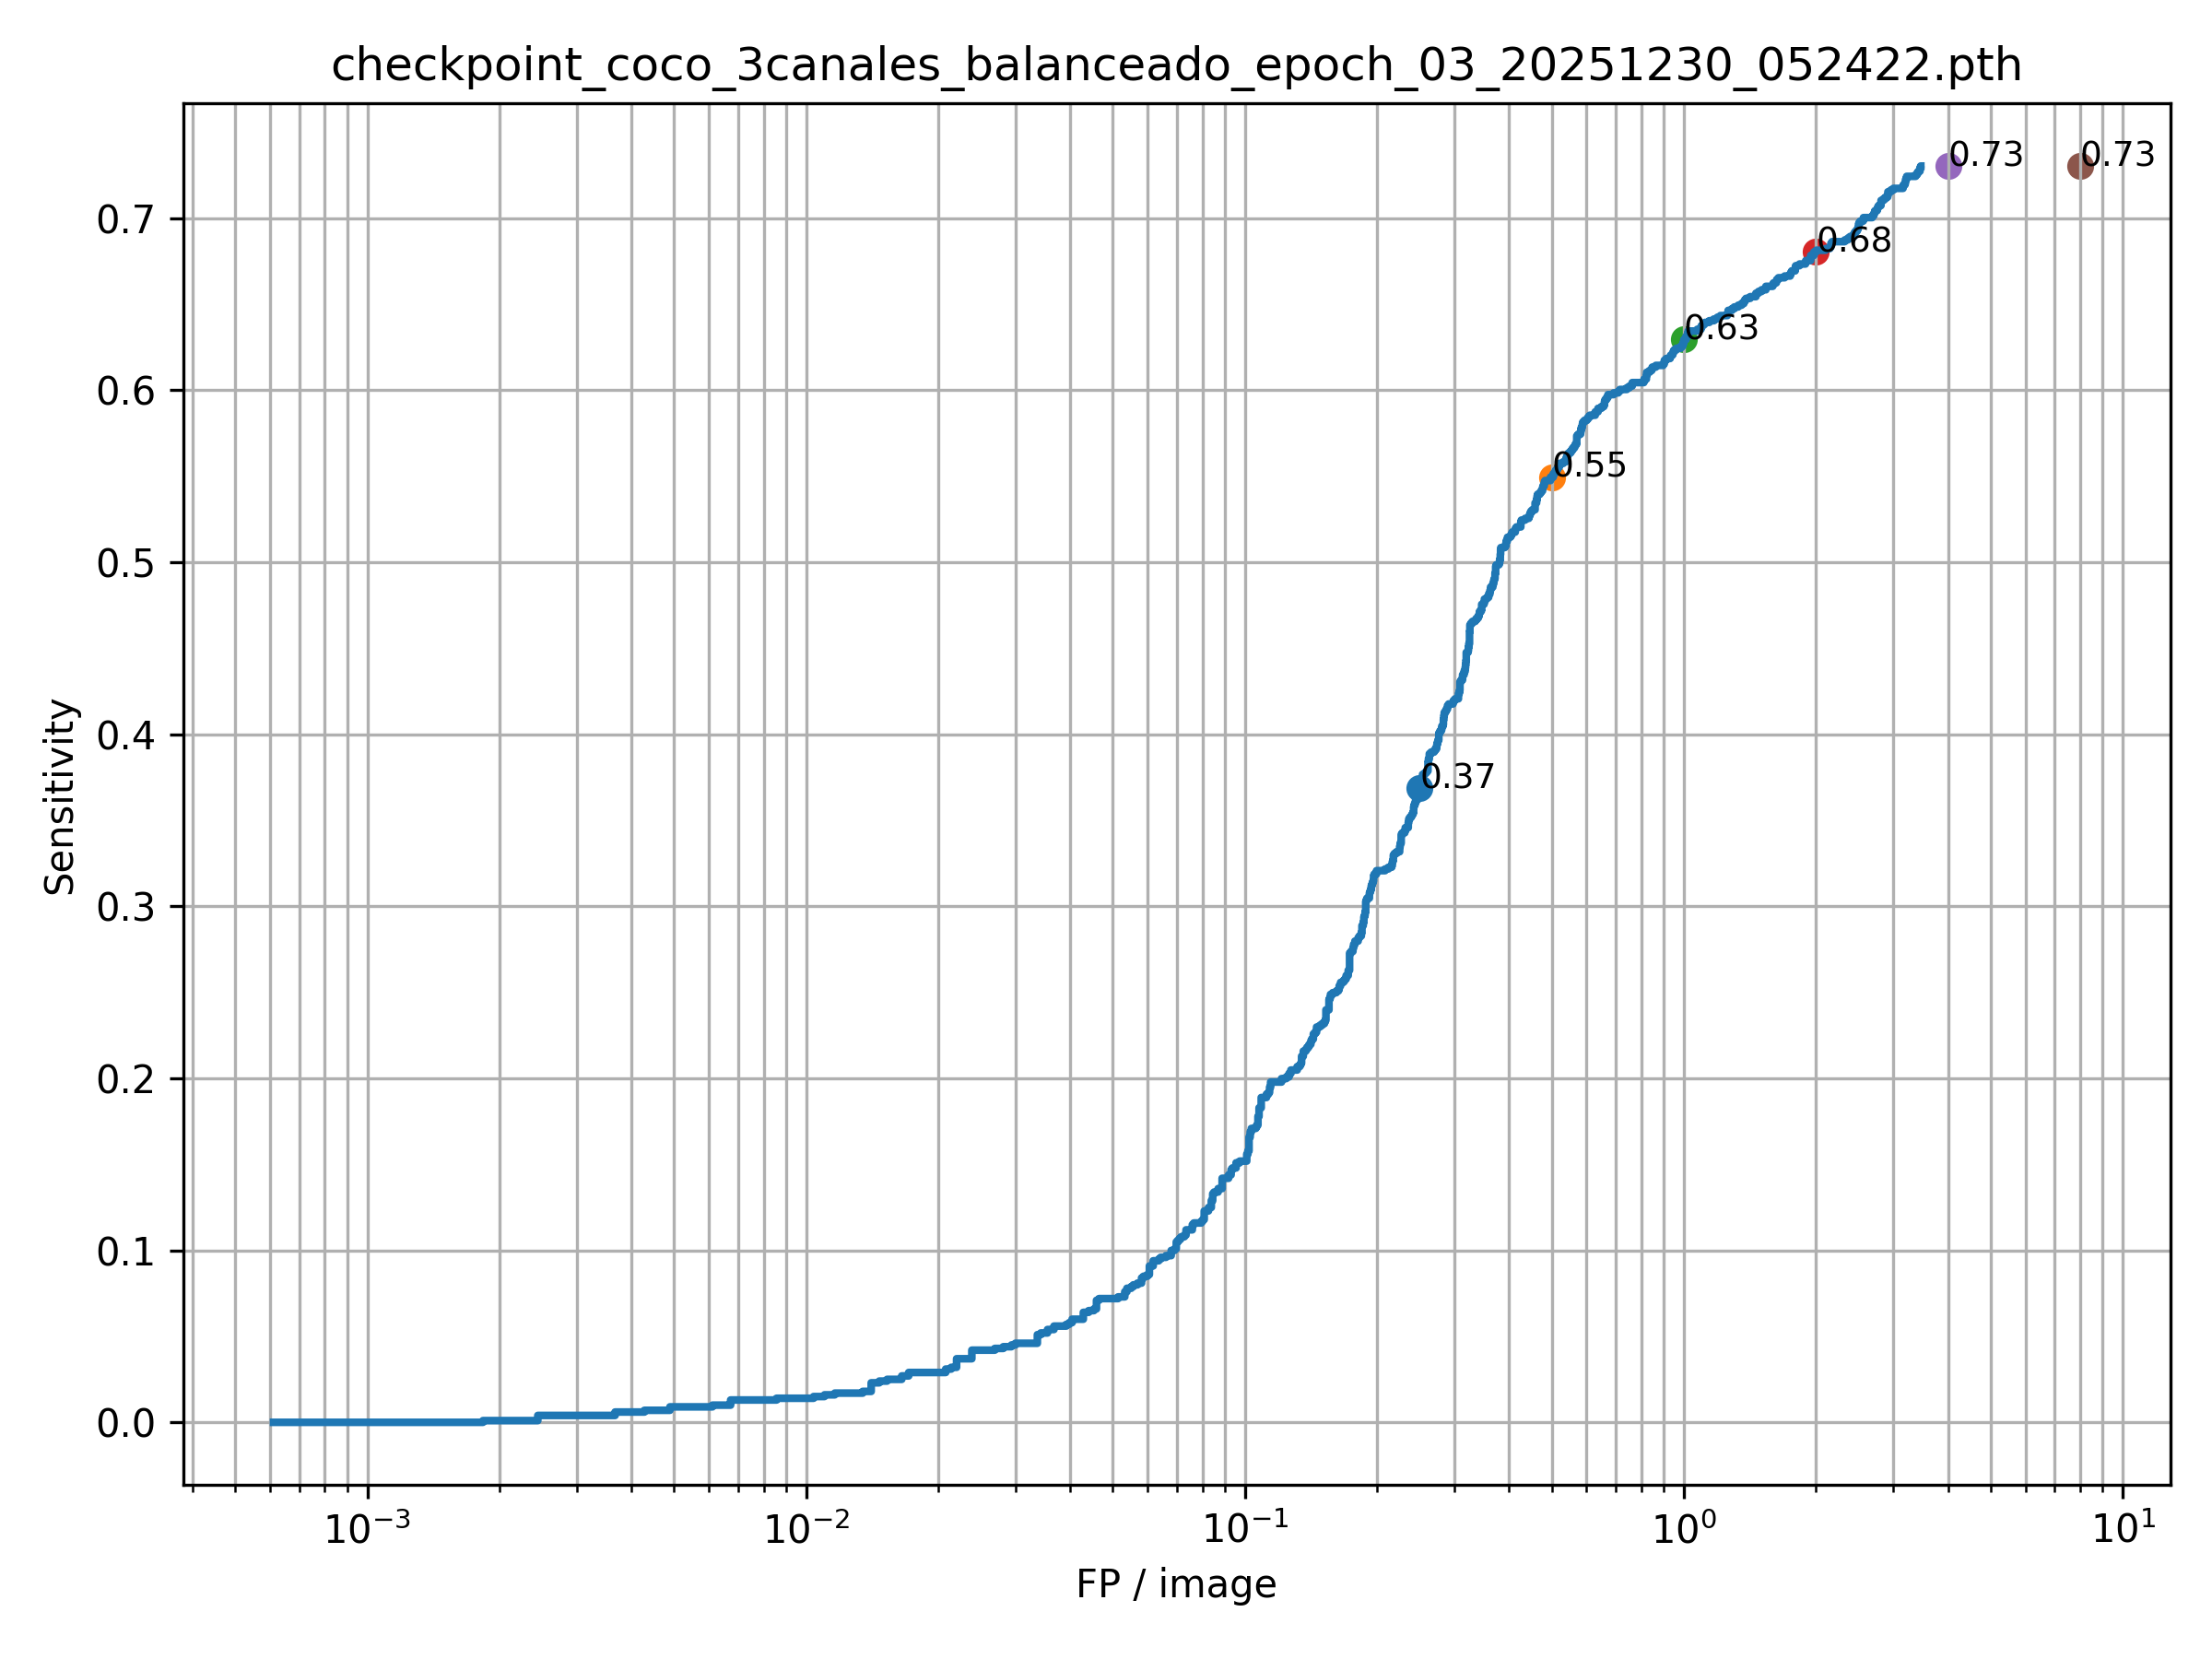
\includegraphics[width=0.8\columnwidth]{images/checkpoint_coco_3canales_balanceado_epoch_03_20251230_052422_froc.png}
    \caption{Corba FROC del millor checkpoint del model Faster R-CNN preentrenat en
    COCO amb representació multicanal (tres canals).}
    \label{fig:model1_coco_3canales_froc}
\end{figure}

En canvi, els resultats obtinguts amb pesos preentrenats en VinDr-CXR mostren un
comportament substancialment diferent. Tant la configuració monocanal com la
multicanal assoleixen valors elevats de sensibilitat i NODE21 score, amb una
lleugera avantatge de la representació multicanal en alguns checkpoints. No
obstant això, la diferència entre ambdues configuracions és reduïda i no es
manifesta de manera uniforme en tots els punts de la corba FROC.

Aquest comportament indica que, un cop el backbone ha estat preentrenat en un
domini radiològic específic, la representació monocanal ja captura la major part
de la informació rellevant per a la detecció de nòduls pulmonars. L’aportació
addicional dels canals CLAHE i \textit{unsharp masking} té un impacte marginal,
millorant lleugerament alguns punts de sensibilitat però sense produir un salt
qualitatiu comparable al derivat del canvi de domini de preentrenament.

En conjunt, aquests resultats posen de manifest que el factor determinant del
rendiment del detector no és tant el nombre de canals d’entrada com l’alineació
entre el domini del preentrenament i la tasca clínica objectiu. El preentrenament
en VinDr-CXR permet aprendre característiques radiològiques específiques que es
transfereixen de manera molt efectiva a la detecció de nòduls pulmonars, mentre
que l’extensió multicanal actua com un refinament secundari amb un impacte
limitat.




% ==================
% # Model 3: Extensions amb Focal Loss i mecanismes d’atenció
% ==================
\subsection{Extensions del model base amb Focal Loss i mecanismes d’atenció}

Un cop establerts els models base de detecció i la seva extensió multicanal, 
es va considerar pertinent explorar algunes estratègies addicionals descrites 
a la literatura recent amb l’objectiu d’analitzar si podien aportar millores 
incrementals en la detecció de nòduls pulmonars \cite{node21challenge,behrendt2023node21}.

Aquest conjunt d’experiments no parteix d’una hipòtesi d’innovació forta, sinó 
d’un enfocament clarament exploratori i formatiu. La seva motivació principal 
prové, d’una banda, de la lectura d’articles recents relacionats amb la millora 
del rendiment en tasques de detecció mitjançant mecanismes d’atenció, i de 
l’altra, de l’anàlisi de les estratègies utilitzades per alguns participants 
del repte NODE21.

En particular, s’ha pres com a referència el treball publicat a 
\textit{Scientific Reports} l’any 2024, en el qual es proposa l’ús combinat 
de mecanismes d’atenció de canal i atenció espacial per reforçar l’extracció 
de característiques rellevants i millorar la localització de nòduls pulmonars 
en imatge mèdica \cite{rehman2024dualattention}. A partir d’aquest marc teòric, 
en aquest treball es planteja la realització de proves preliminars d’integració 
de mecanismes d’atenció en el pipeline de detecció, amb l’objectiu d’avaluar 
si aquests poden contribuir a una millor discriminació de les regions d’interès.

De manera complementària, i atenent a la problemàtica de desbalanceig de classes 
habitual en la detecció de nòduls pulmonars, també es proposa analitzar l’ús de 
funcions de pèrdua alternatives, com la \textit{Focal Loss}, descrita a la 
literatura com una estratègia efectiva per penalitzar de manera més severa 
els exemples difícils i reduir l’impacte dels falsos positius. En aquest context, 
la seva incorporació es concep com una extensió experimental destinada a estudiar 
el seu possible impacte en el rendiment del model.

Cal remarcar que totes les proves descrites en aquesta secció es realitzen 
mantenint com a punt de partida el model Faster R-CNN preentrenat en VinDr-CXR, 
entrenat sobre dades balancejades mitjançant estratègies de \textit{data 
augmentation}, tal com s’ha fet de manera sistemàtica al llarg de tot el treball. 
Aquest plantejament permet aïllar l’impacte real de cada modificació introduïda 
i avaluar de manera controlada la contribució de les estratègies explorades.



% ==================
% # Focal Loss
% ==================

\subsubsection{Introducció de Focal Loss}

Tot i que el conjunt de dades utilitzat en aquest treball es construeix de manera
balancejada mitjançant \textit{data augmentation}, la detecció de nòduls pulmonars
presenta inherentment un desequilibri a nivell de dificultat: la majoria de regions
proposades corresponen a fons, mentre que els nòduls constitueixen objectes petits,
amb poc contrast i fàcilment confusos amb estructures anatòmiques normals.

Motivats per aquesta observació, i seguint propostes àmpliament utilitzades en detecció
d’objectes, es va experimentar amb la substitució de la funció de pèrdua de classificació
estàndard per una \textit{Focal Loss}. Aquesta funció penalitza amb més intensitat els
exemples difícils i redueix el pes dels exemples fàcilment classificables, afavorint així
l’aprenentatge en escenaris amb dominància de fons.

Des del punt de vista de la implementació, la modificació es limita exclusivament a la
definició de la funció de pèrdua associada a la capçalera de classificació del Faster
R-CNN. La resta del pipeline —arquitectura, estratègia de congelació del backbone,
hiperparàmetres d’entrenament i procediment d’avaluació— es manté idèntica al model
base, garantint així una comparació justa.

Aquesta prova permet analitzar si, fins i tot en un escenari amb dades balancejades,
la Focal Loss pot aportar beneficis addicionals en la detecció de nòduls petits o de
difícil localització.

Els resultats obtinguts amb la introducció de la \textit{Focal Loss} mostren un
comportament molt similar al del model Faster R-CNN preentrenat en VinDr-CXR
 entrenat amb funció de pèrdua estàndard. En ambdós
casos, el model assoleix un \textit{NODE21 score} proper a 0.89, amb una sensibilitat
al voltant del 0.76 a 0.25 falsos positius per imatge, incrementant-se de manera
progressiva fins a valors superiors al 0.92 a partir d’1 fals positiu per imatge.

Aquest comportament es reflecteix a la Figura~\ref{fig:vindr_focal_froc}, on es pot
observar una corba FROC molt estable en tots els règims d’operació analitzats. En
particular, el model manté una elevada sensibilitat sense penalitzacions rellevants
en el nombre de falsos positius, fet especialment important en un context clínic.

\begin{figure}[H]
    \centering
    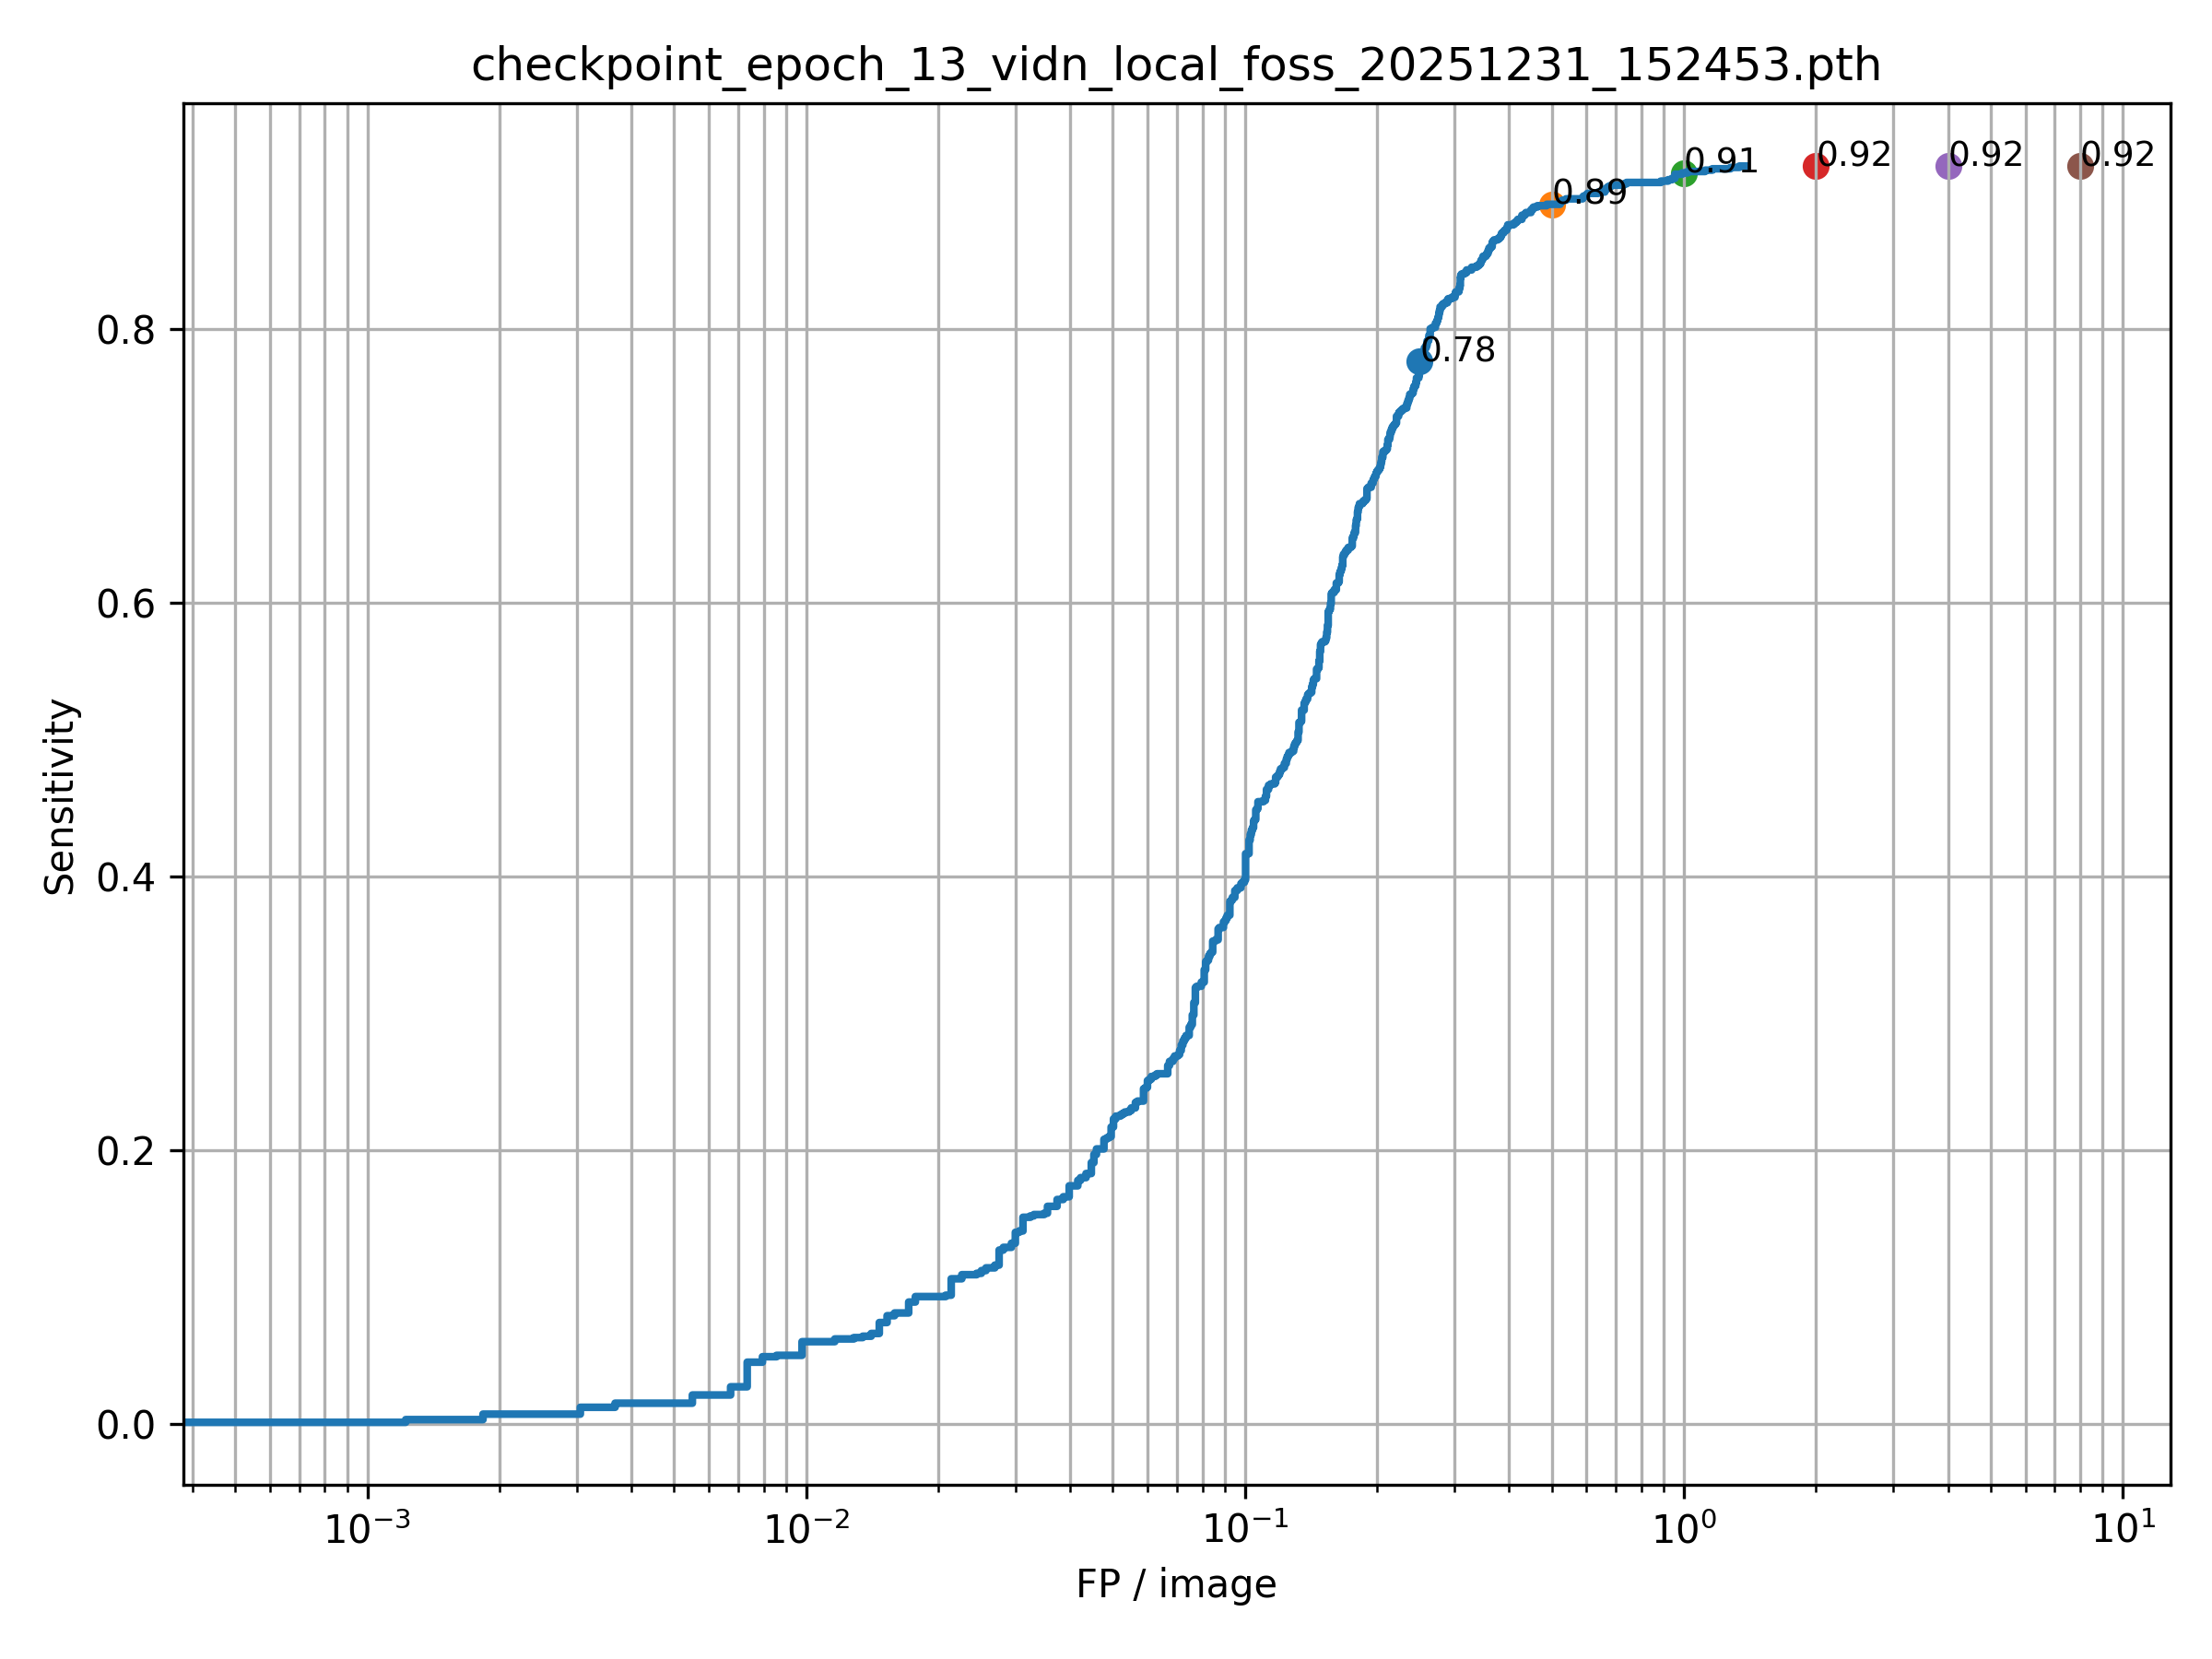
\includegraphics[width=0.8\columnwidth]{images/checkpoint_epoch_13_vidn_local_foss_20251231_152453_froc.png}
    \caption{Corba FROC del millor model Faster R-CNN preentrenat en VinDr-CXR amb
    representació multicanal i funció de pèrdua \textit{Focal Loss}. Els punts
    ressaltats indiquen els nivells de sensibilitat assolits als valors de falsos
    positius per imatge utilitzats en l’avaluació oficial del repte NODE21.}
    \label{fig:vindr_focal_froc}
\end{figure}



Els valors puntuals de sensibilitat obtinguts pel millor model multicanal amb
preentrenament VinDr-CXR són:
\begin{table}[H]
\centering
\footnotesize
\caption{Sensibilitat del model Faster R-CNN preentrenat en VinDr-CXR amb funció de pèrdua \textit{Focal Loss} a diferents nivells de falsos positius per imatge}
\label{tab:vindr_focal_sensitivity}
\setlength{\tabcolsep}{6pt}
\begin{tabular}{cc}
\toprule
\textbf{FP per imatge} & \textbf{Sensibilitat} \\
\midrule
0.25 & 0.758 \\
0.5  & 0.892 \\
1    & 0.916 \\
2    & 0.927 \\
4    & 0.927 \\
8    & 0.927 \\
\bottomrule
\end{tabular}
\end{table}


En conjunt, aquests resultats suggereixen que la millora clau en la detecció de
nòduls pulmonars prové principalment de l’alineació del domini de preentrenament
(VinDr-CXR) amb la naturalesa radiològica de la tasca, així com de l’ús d’una
representació multicanal informativament rica. En aquest escenari, la Focal Loss
actua com un mecanisme de regularització que manté el rendiment, però no introdueix
guanys addicionals significatius sobre una configuració ja fortament optimitzada.


% ==================
% # Mecanismes d’atenció
% ==================

\subsubsection{Incorporació de mecanismes d’atenció}

Paral·lelament a l’exploració de la Focal Loss,  es va considerar d’interès explorar la incorporació de
mecanismes d’atenció com a possible via de millora incremental del rendiment.

La motivació principal d’aquestes proves prové de la lectura de treballs recents en la
literatura, en particular l’article publicat a \textit{Scientific Reports} l’any 2024,
on es proposa l’ús combinat de mecanismes d’atenció de canal i espacial per millorar la
detecció de nòduls pulmonars en imatge mèdica \cite{scirep2024_attention}. En aquest
treball, els autors mostren que els mecanismes d’atenció poden ajudar el model a
ressaltar patrons rellevants i a suprimir informació redundant en entorns visuals
complexos.

Cal remarcar que l’objectiu d’aquesta secció no és reproduir fidelment l’arquitectura
proposada en el treball citat, sinó analitzar de manera controlada l’impacte de diferents
estratègies d’atenció integrades dins d’un detector estàndard com Faster R-CNN. Totes les
proves es realitzen mantenint constant el backbone, l’estratègia d’entrenament i el
procediment d’avaluació, prenent com a base el model preentrenat en VinDr-CXR amb dades
balancejades.

\subsubsection{Atenció aplicada a les Regions of Interest (RoI)}

En una primera aproximació, es va implementar un mecanisme d’atenció aplicat directament
sobre les característiques extretes a nivell de les \textit{Regions of Interest} (RoI).
Aquesta estratègia pretén reforçar les representacions associades a regions candidates
potencialment rellevants abans de la classificació final, sense modificar el procés de
proposta de regions ni el backbone convolucional.

Des del punt de vista pràctic, aquesta variant introdueix una modulació lleugera de les
característiques RoI mitjançant una capa d’atenció addicional, mantenint intacta la resta
de l’arquitectura Faster R-CNN. L’objectiu és avaluar si una reponderació local de les
característiques pot facilitar la discriminació entre nòduls reals i estructures
anatòmiques confusores.

Els resultats obtinguts amb aquesta variant mostren un comportament molt similar al del
model base. El millor checkpoint amb atenció a nivell RoI assoleix un \textit{NODE21 score}
proper a \textbf{0.895}, amb una sensibilitat al voltant de \textbf{0.76} a 0.25 falsos
positius per imatge, augmentant fins a valors pròxims o superiors a \textbf{0.93} a partir
d’1 fals positiu per imatge.

La Figura~\ref{fig:vindr_roi_froc} mostra la corba FROC corresponent a aquesta configuració,
on s’observa una evolució estable i pràcticament superposada a la del model sense
atenció, especialment en els règims d’operació clínicament més rellevants.

\begin{figure}[H]
    \centering
    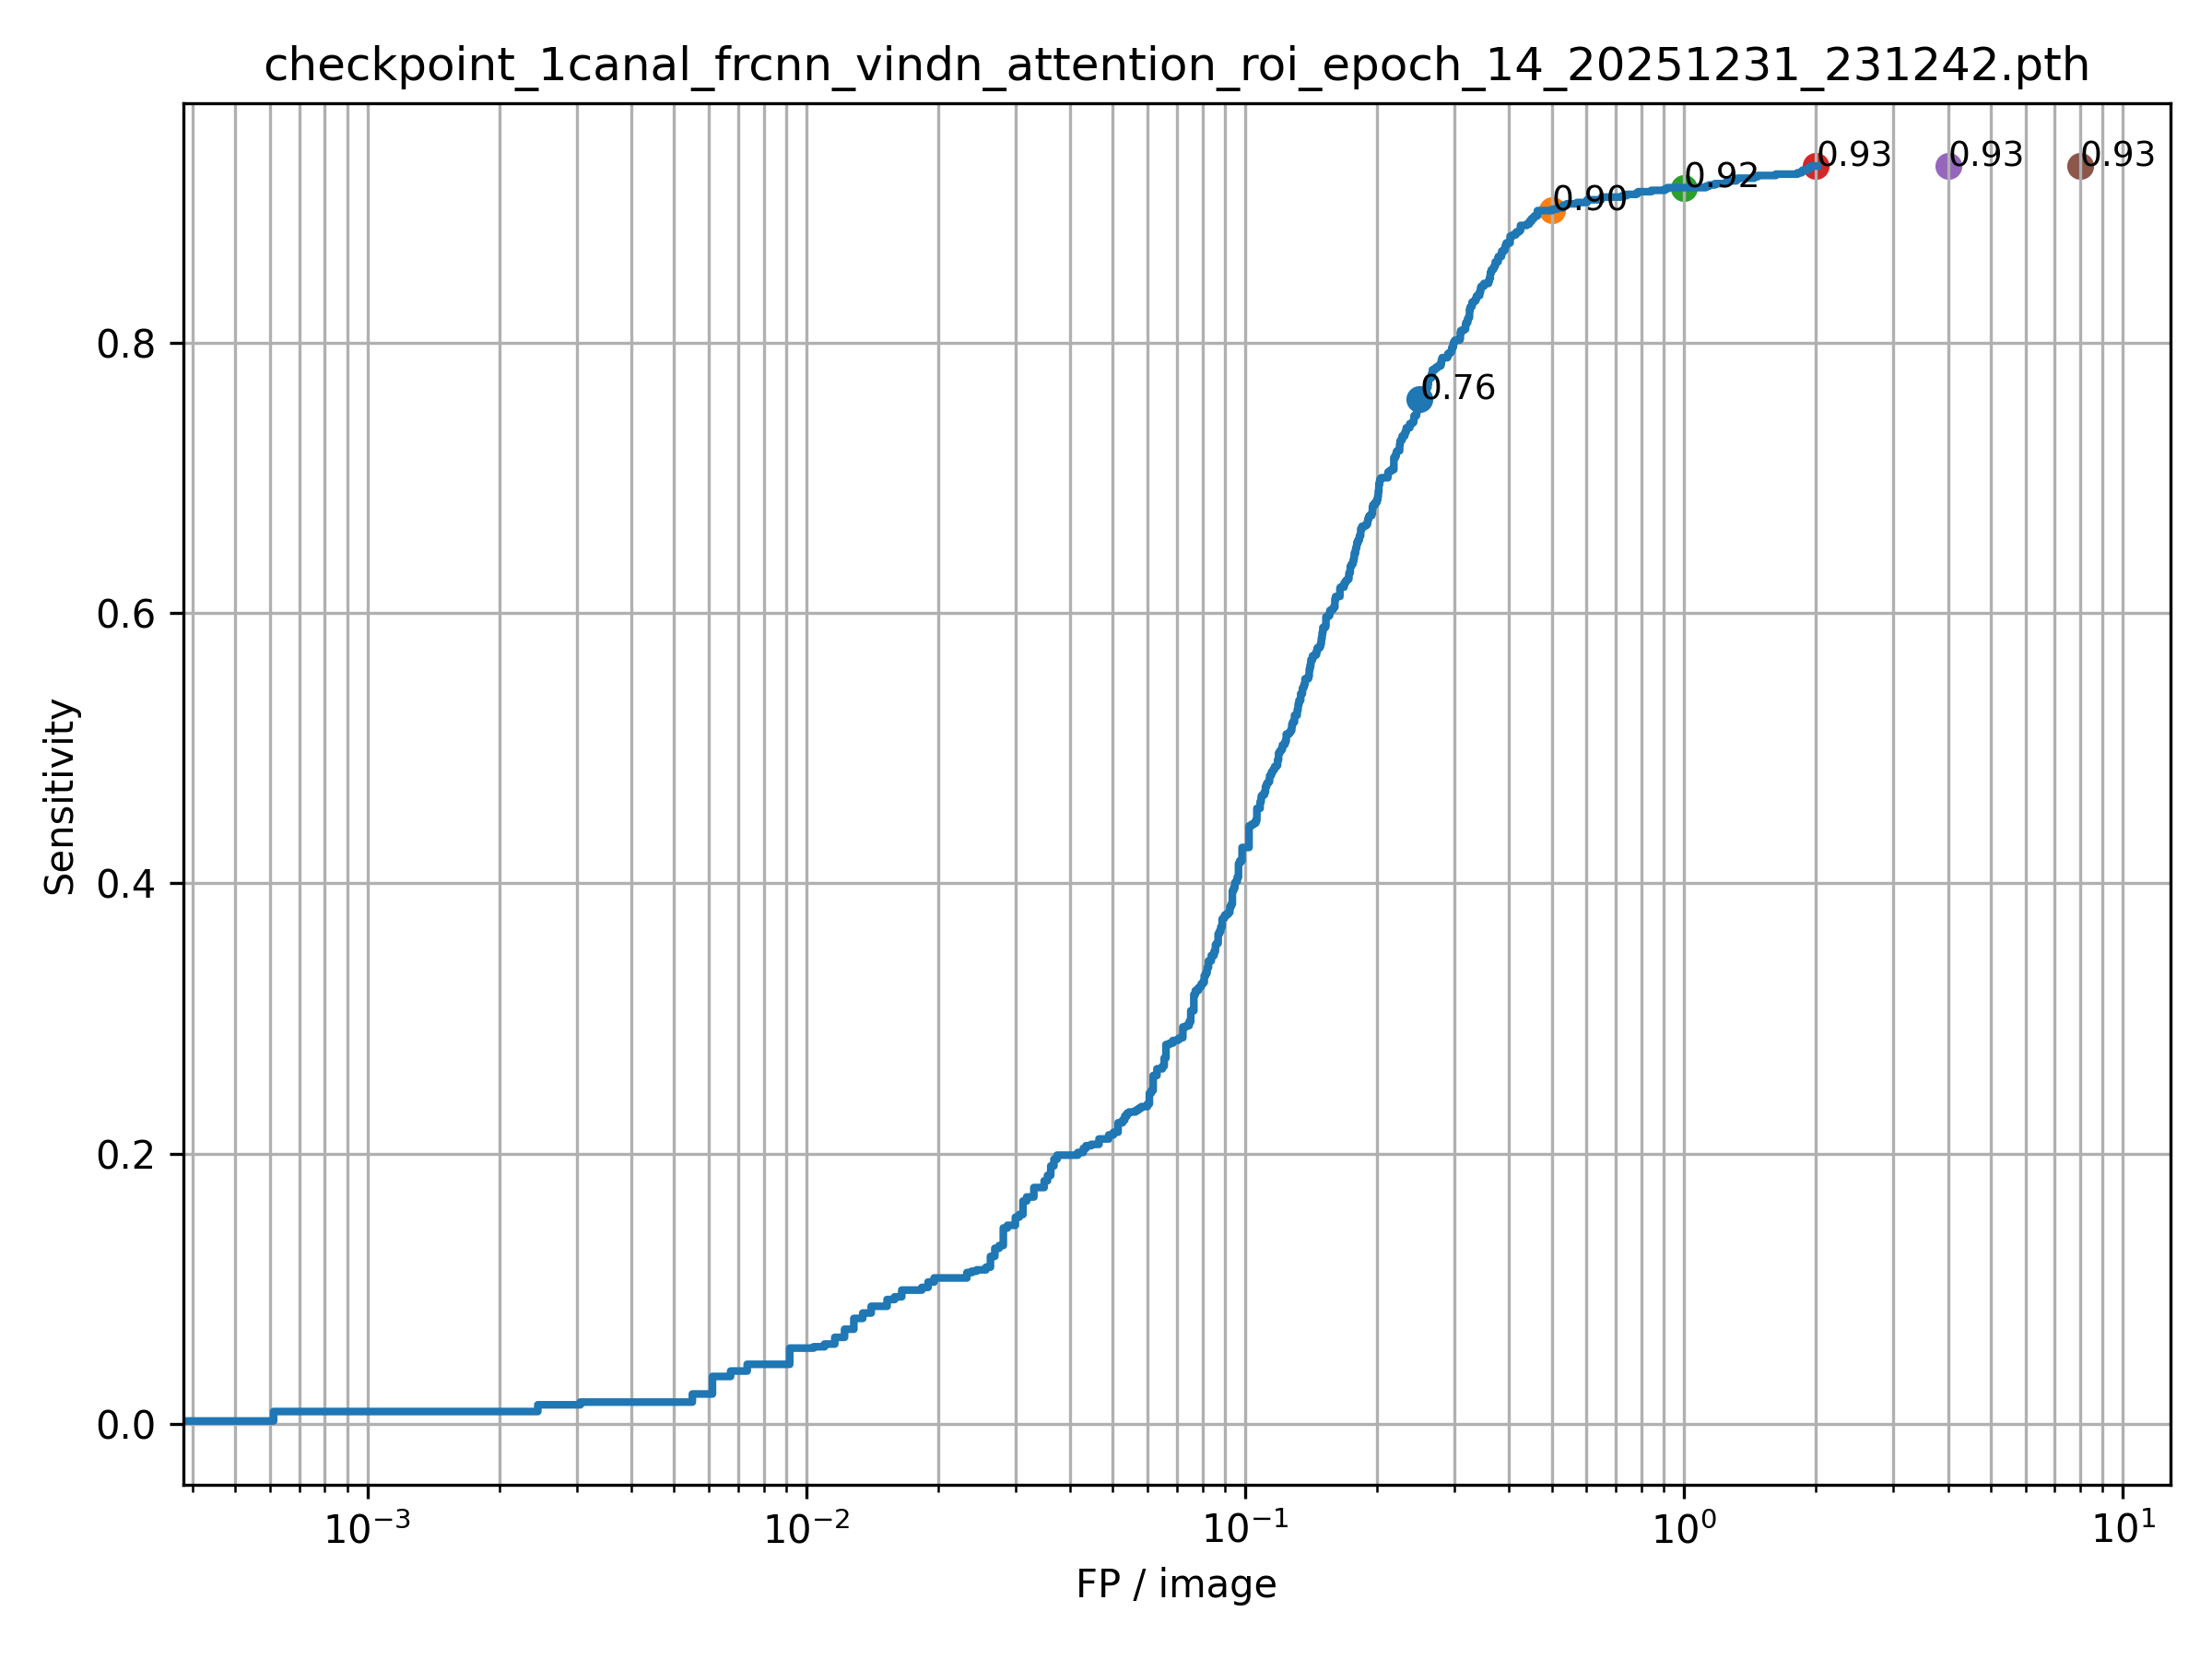
\includegraphics[width=0.85\columnwidth]{images/checkpoint_1canal_frcnn_vindn_attention_roi_epoch_14_20251231_231242_froc.png}
    \caption{Corba FROC del millor model Faster R-CNN preentrenat en VinDr-CXR amb
    mecanisme d’atenció aplicat a nivell de Regions of Interest (RoI).}
    \label{fig:vindr_roi_froc}
\end{figure}

\subsubsection{Atenció dual de tipus CBAM}

En una segona fase, es va implementar un mecanisme d’atenció més complet basat en el mòdul
CBAM (\textit{Convolutional Block Attention Module}), que combina de manera seqüencial
atenció de canal i atenció espacial. Aquesta aproximació està directament inspirada en
la literatura recent, on s’ha demostrat que la combinació d’ambdós tipus d’atenció permet
al model identificar tant \textit{què} és rellevant (canals informatius) com \textit{on}
es localitza la informació rellevant dins la imatge \cite{scirep2024_attention}.

En el context de la detecció de nòduls pulmonars, aquesta doble perspectiva resulta
especialment atractiva, atès que els nòduls solen ser petits, de baix contrast i immersos
en estructures anatòmiques complexes. La integració del mòdul CBAM es realitza de manera
modular, sense alterar la resta del pipeline del detector, permetent així una avaluació
aïllada del seu impacte.

Els resultats obtinguts amb aquesta configuració mostren un rendiment molt proper al del
model base i a la variant amb atenció RoI. El millor checkpoint amb atenció CBAM assoleix
un \textit{NODE21 score} de \textbf{0.892}, amb una sensibilitat de \textbf{0.762} a
0.25 FP/img, incrementant-se fins a valors d’aproximadament \textbf{0.93} a partir d’1
fals positiu per imatge.

A la Figura~\ref{fig:vindr_cbam_froc} es presenta la corba FROC corresponent a aquesta
variant. Es pot observar que el comportament global és molt estable i coherent amb la
resta de configuracions, sense penalitzacions significatives en cap règim d’operació.

\begin{figure}[H]
    \centering
    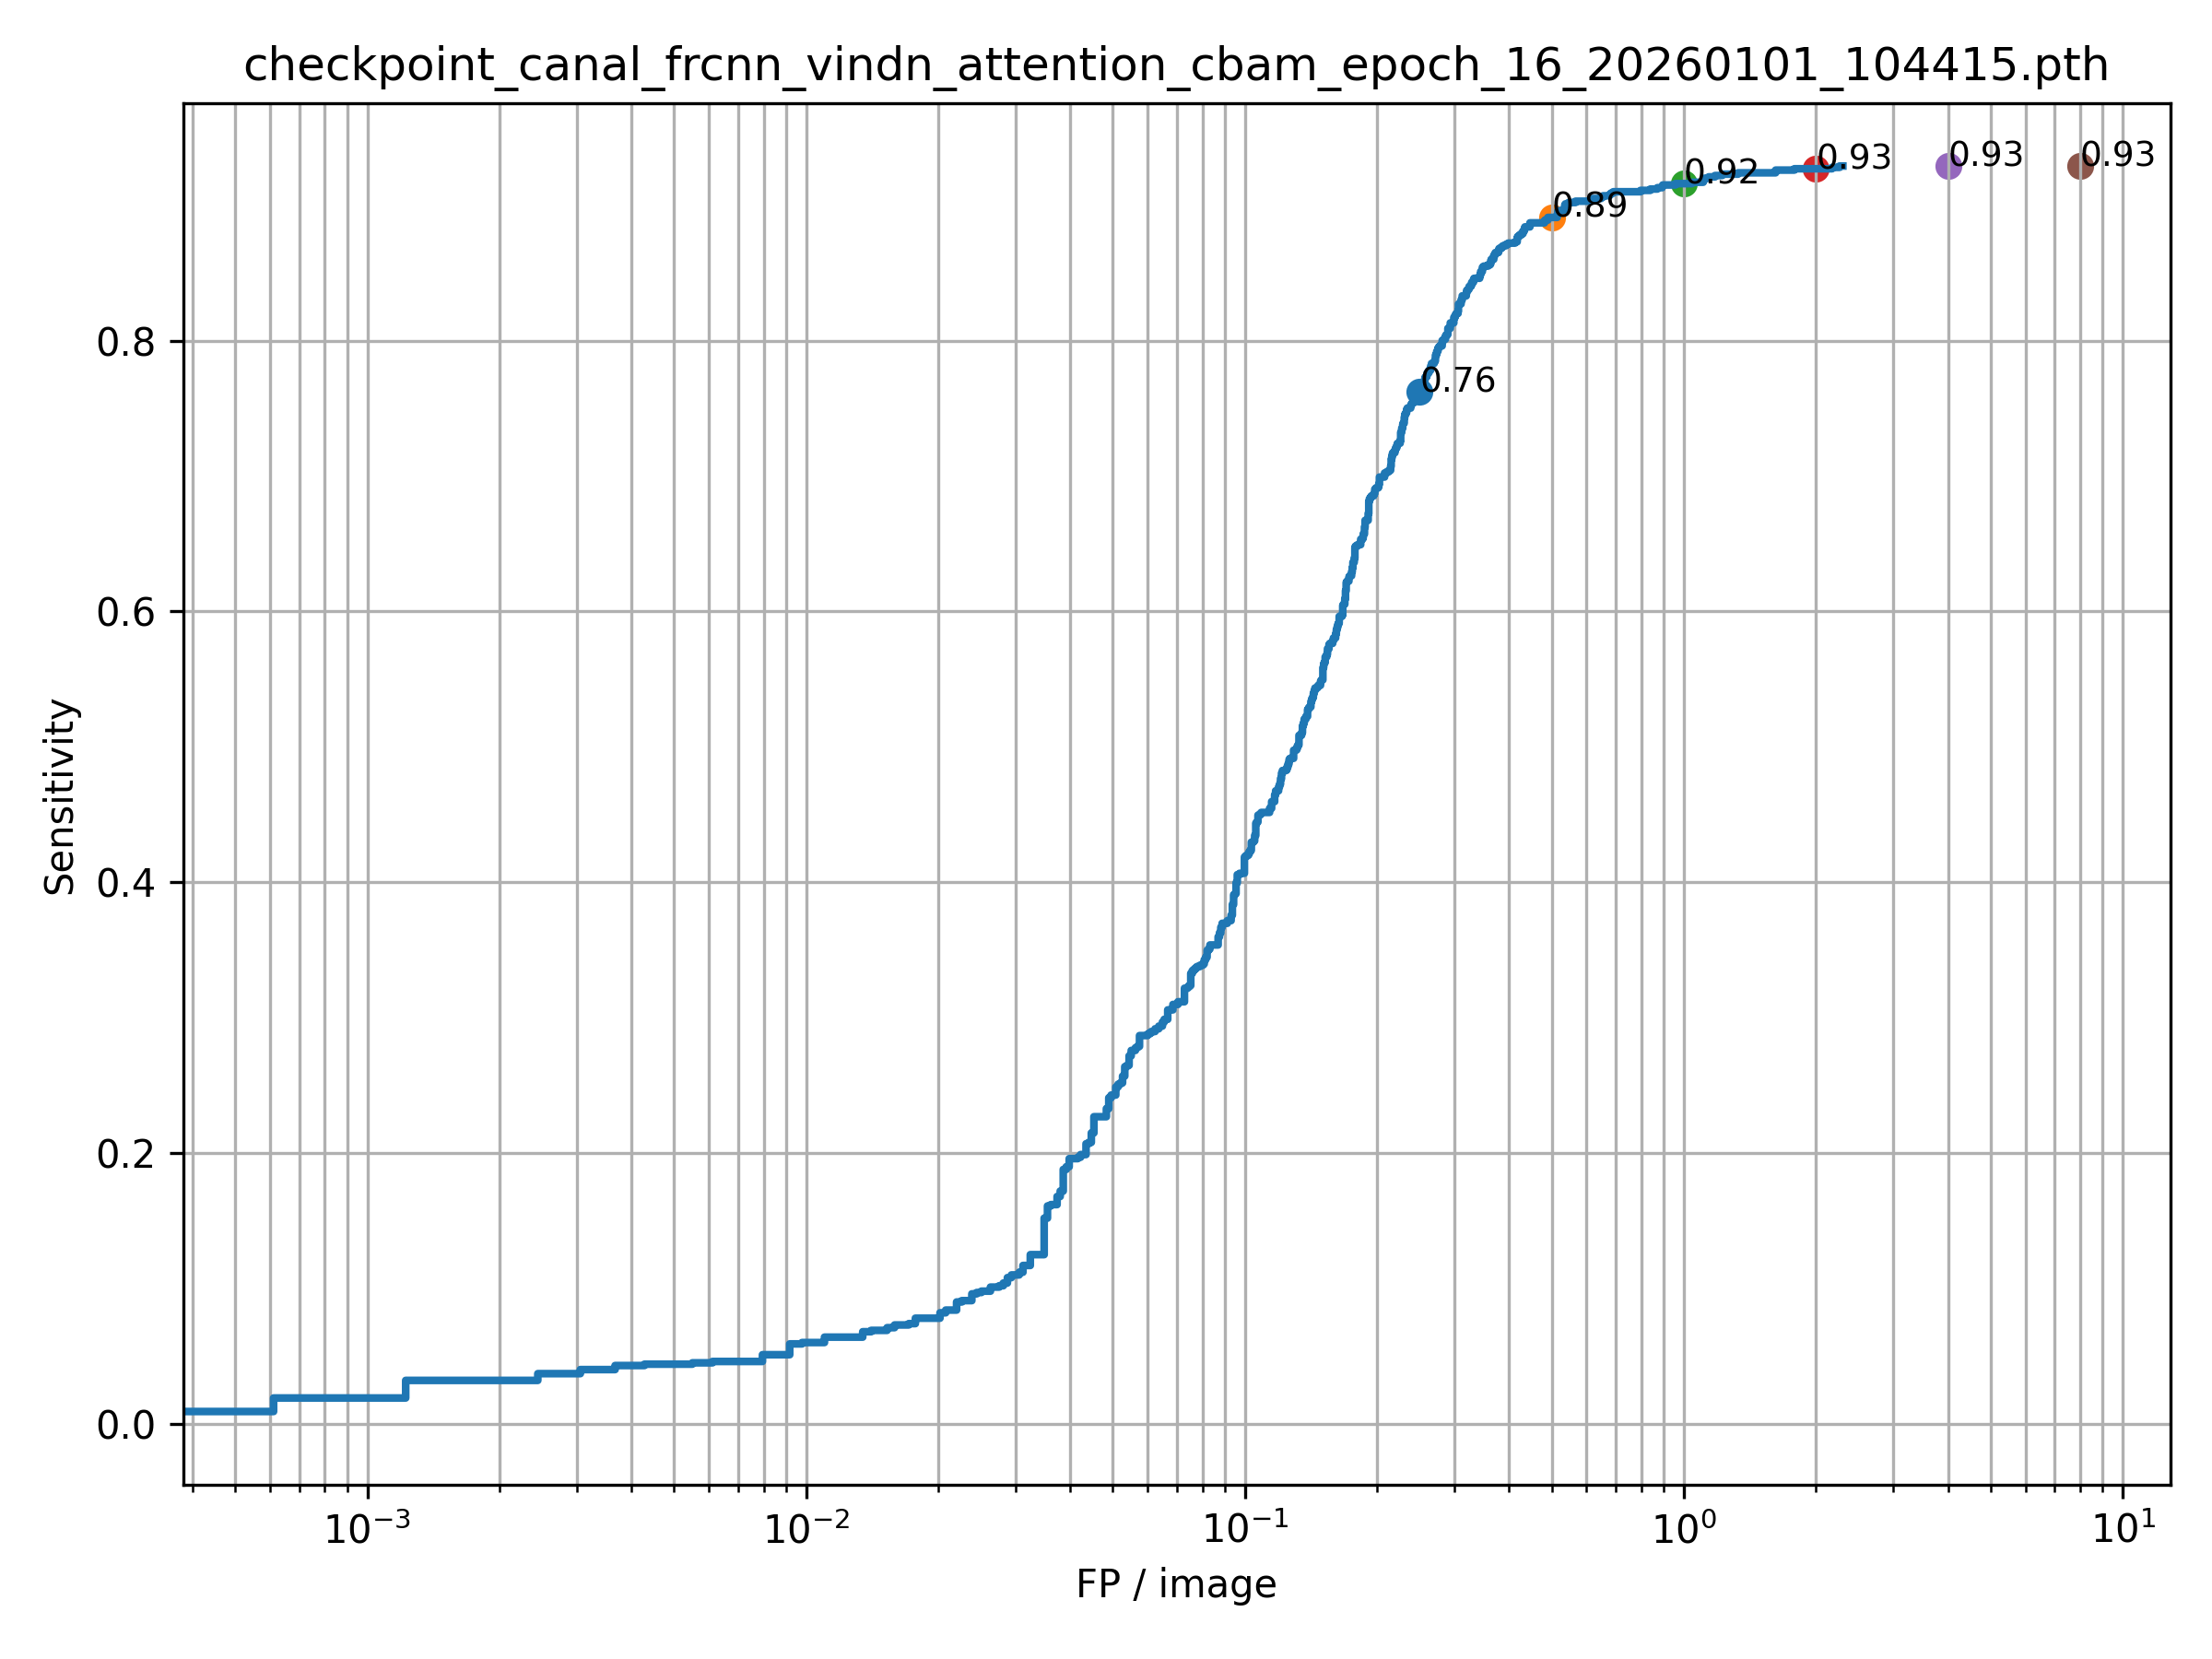
\includegraphics[width=0.85\columnwidth]{images/checkpoint_canal_frcnn_vindn_attention_cbam_epoch_16_20260101_104415_froc.png}
    \caption{Corba FROC del millor model Faster R-CNN preentrenat en VinDr-CXR amb
    mecanisme d’atenció dual de tipus CBAM.}
    \label{fig:vindr_cbam_froc}
\end{figure}

En conjunt, els resultats obtinguts amb els diferents mecanismes d’atenció suggereixen
que, en un escenari ja fortament optimitzat mitjançant un preentrenament adequat
(VinDr-CXR) i una representació multicanal informativa, la incorporació d’atenció no
produeix guanys substancials addicionals. Tanmateix, aquestes proves confirmen que els
mecanismes d’atenció poden integrar-se sense degradar el rendiment i aporten una
validació empírica de les tendències descrites a la literatura recent.


% ==================
% # Model 3: Detecció de nòduls pulmonars amb RetinaNet
% ==================

\section{Model 3: Detecció de nòduls pulmonars amb RetinaNet}

Després d’avaluar arquitectures de detecció de dues etapes basades en Faster R-CNN amb diferents estratègies de preentrenament, es va explorar un tercer enfocament basat en \textit{RetinaNet}, un detector d’una sola etapa dissenyat per abordar de manera explícita el problema del desequilibri entre classes mitjançant la funció de pèrdua \textit{Focal Loss}.

RetinaNet combina un \textit{backbone} convolucional amb una \textit{Feature Pyramid Network} (FPN) per a l’extracció multiescala de característiques, juntament amb dos caps especialitzats per a classificació i regressió de caixes delimitadores. En aquest treball s’ha utilitzat una arquitectura \textbf{ResNet50-FPN} preentrenada sobre el conjunt de dades \textit{COCO}, adaptada posteriorment a la tasca específica de detecció de nòduls pulmonars en radiografies de tòrax.

Atès que les imatges originals són monocanal, les radiografies s’han convertit a format PNG i normalitzat, replicant el canal únic per obtenir una entrada de tres canals compatible amb el model preentrenat. Les anotacions del conjunt de dades NODE21 s’han reinterpretat com a \textit{bounding boxes} en coordenades absolutes, preservant totes les anotacions positives associades a cada imatge.

La divisió del conjunt de dades s’ha realitzat a nivell d’imatge, assegurant una separació estricta entre els conjunts d’entrenament i validació per evitar \textit{data leakage}. El conjunt d’entrenament correspon aproximadament al 80\% de les imatges disponibles, mentre que el 20\% restant s’ha reservat per a validació.

Durant el procés d’entrenament, s’han congelat totes les capes del \textit{backbone} excepte el bloc \texttt{layer4}, així com les capes de la FPN i el cap de detecció, amb l’objectiu de reduir el risc de sobreajustament i estabilitzar l’aprenentatge. A més, les capes de \textit{Batch Normalization} s’han mantingut en mode d’avaluació per preservar les estadístiques apreses durant el preentrenament.

El cap de classificació original s’ha substituït per un de nou amb dues classes (fons i nòdul), inicialitzant el biaix de la capa logística amb un valor negatiu calculat a partir d’una probabilitat \textit{a priori} baixa de presència de nòduls, seguint les recomanacions habituals per a detectors amb fort desequilibri de classes.

L’entrenament s’ha dut a terme utilitzant l’optimitzador \textbf{AdamW}, amb una taxa d’aprenentatge inicial reduïda i una estratègia de disminució esglaonada del \textit{learning rate}. El procés inclou mecanismes de \textit{checkpointing} per època i selecció automàtica del millor model segons la pèrdua de validació. Addicionalment, s’ha implementat un criteri d’aturada primerenca (\textit{early stopping}) per prevenir entrenaments innecessaris un cop la pèrdua de validació deixa de millorar.




\subsection{Resultats quantitatius del model basat en RetinaNet}

Un cop finalitzat l’entrenament inicial del model RetinaNet amb backbone
ResNet50-FPN preentrenat en COCO, s’ha procedit a la seva avaluació quantitativa
sobre el conjunt de validació de NODE21 utilitzant el mateix pipeline
d’inferència i les mateixes mètriques emprades en la resta de models, amb
l’objectiu de garantir una comparació directa i justa.

La Figura~\ref{fig:retinanet_froc} mostra la corba FROC corresponent al millor
checkpoint obtingut (\texttt{epoch 04}). El model assoleix un
\textbf{NODE21 score de 0.742}, evidenciant un rendiment competitiu dins del
conjunt de models avaluats, especialment en règims de falsos positius mitjans i
alts.

\begin{figure}[H]
    \centering
    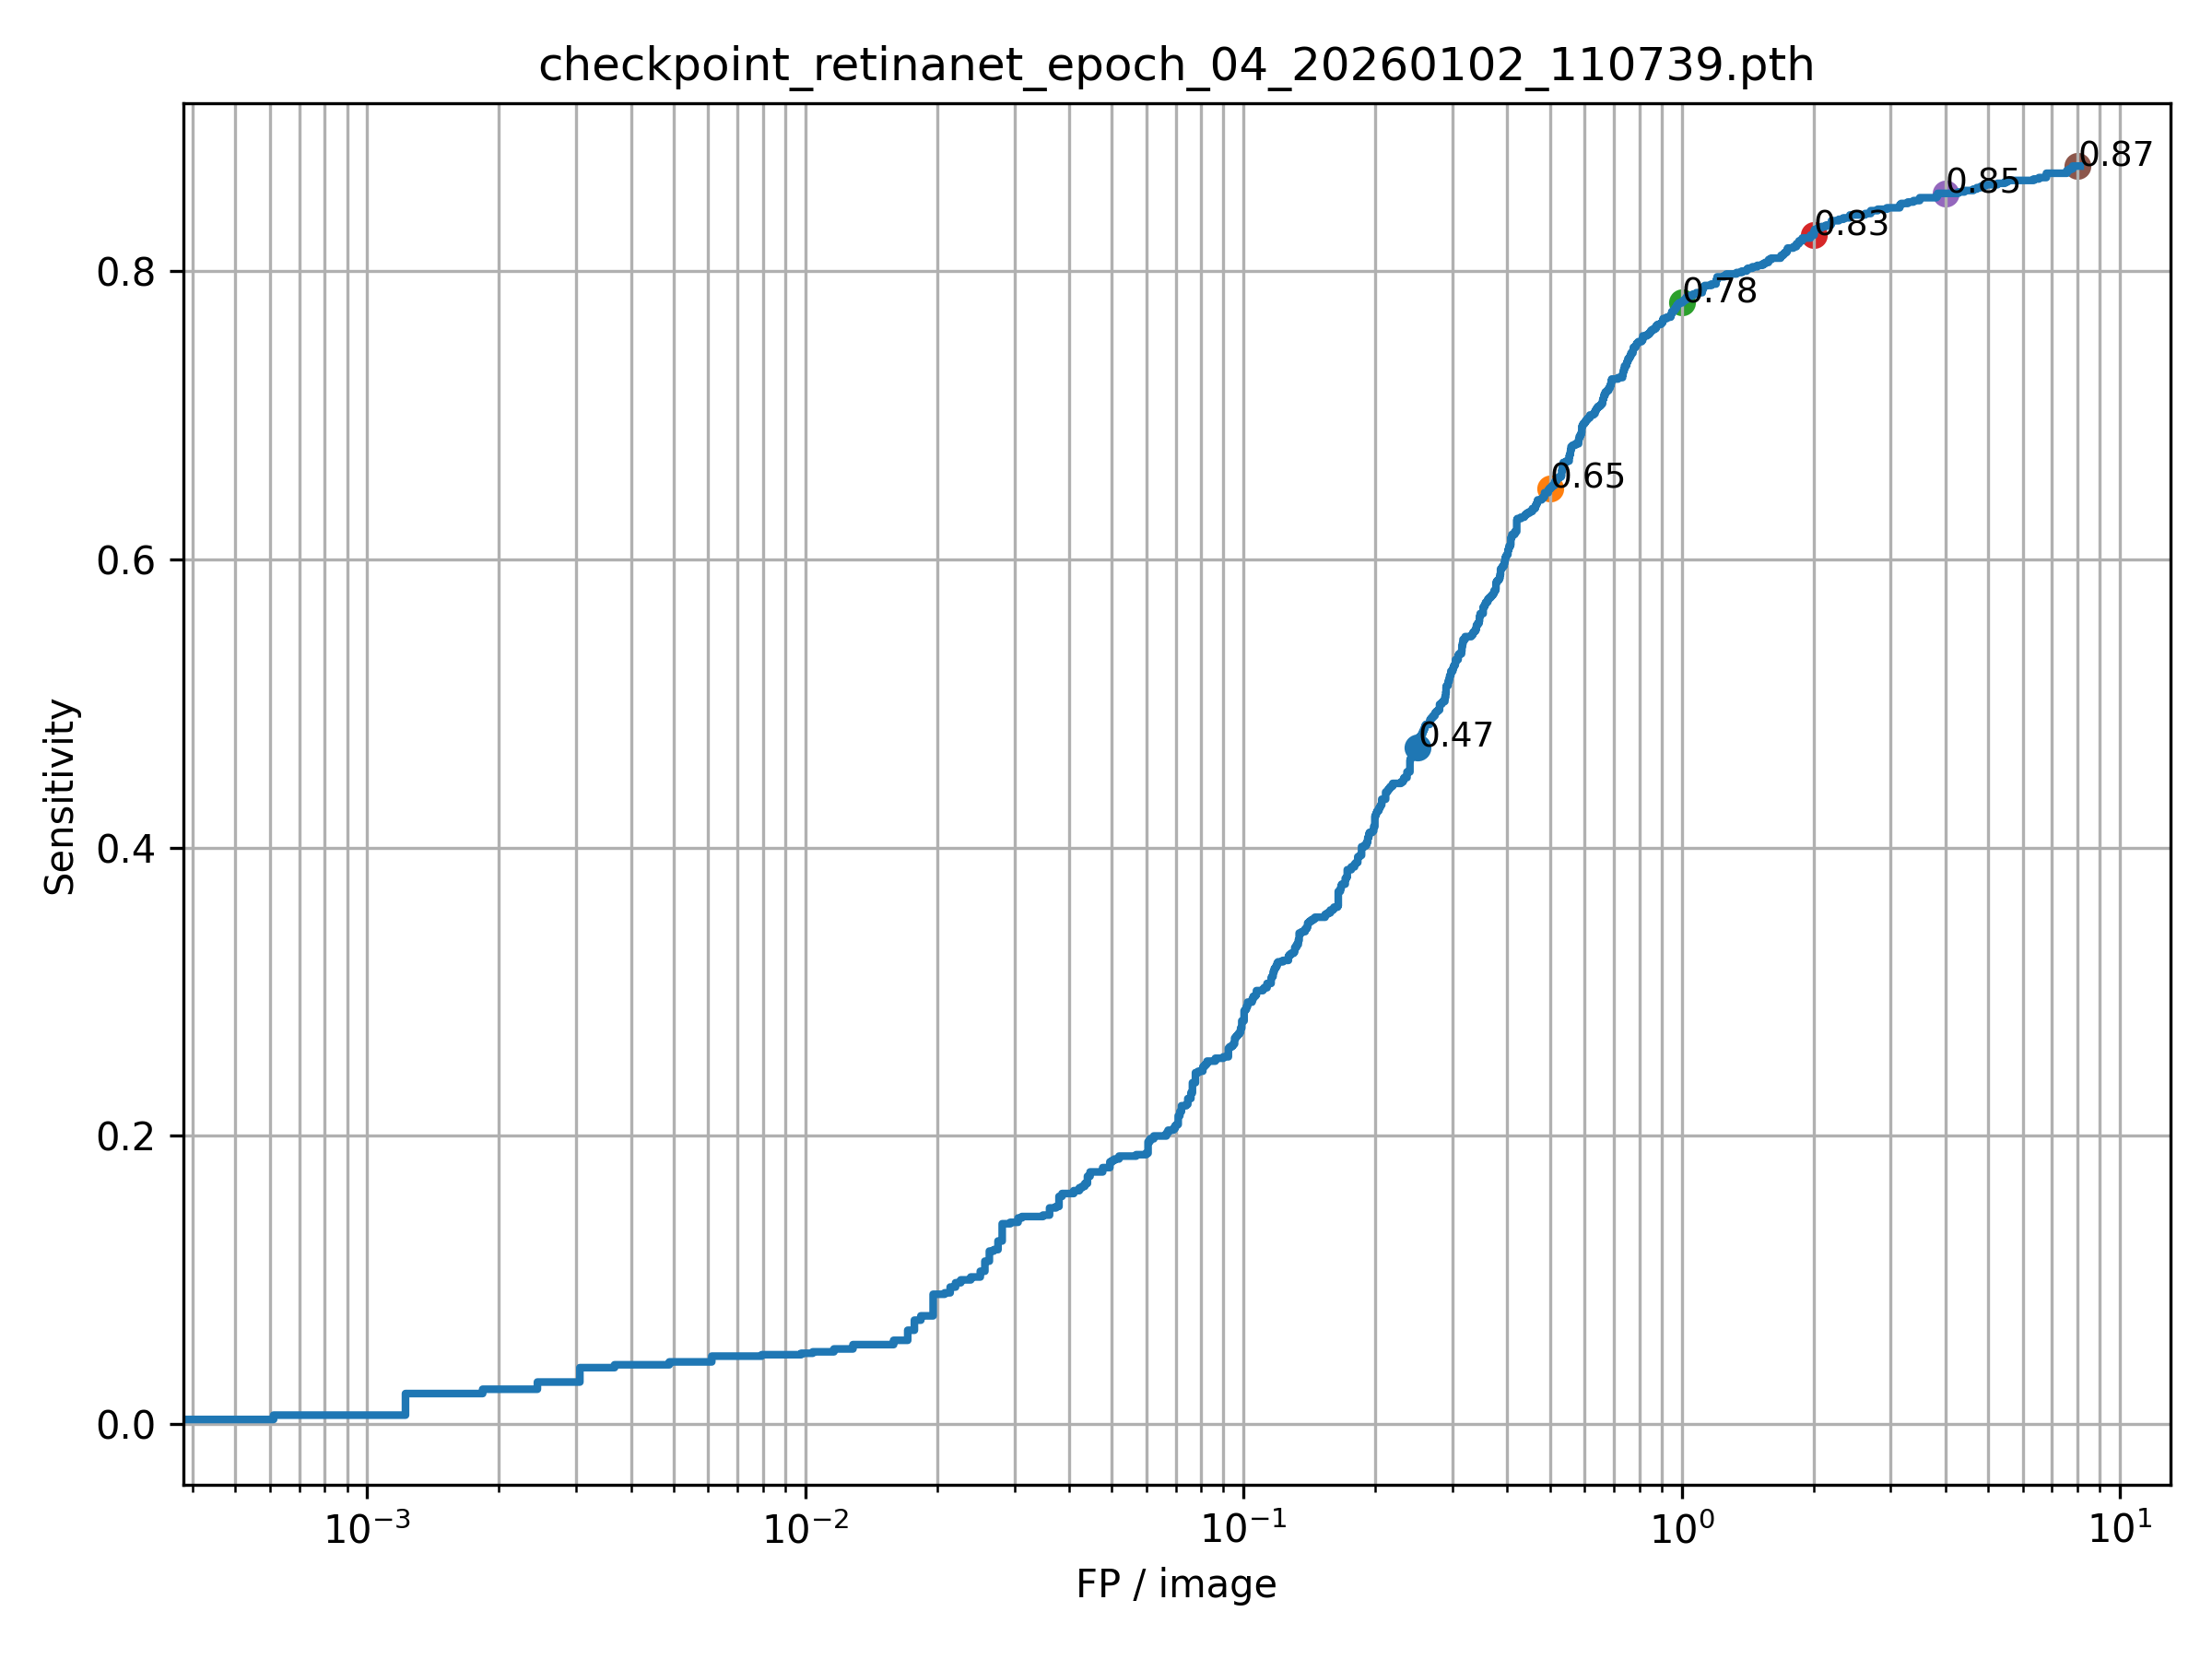
\includegraphics[width=0.8\columnwidth]{images/checkpoint_retinanet_epoch_04_20260102_110739_froc.png}
    \caption{Corba FROC del millor checkpoint del model RetinaNet. Els punts
    ressaltats indiquen els valors de sensibilitat als nivells de falsos positius
    per imatge utilitzats en l’avaluació oficial del repte NODE21.}
    \label{fig:retinanet_froc}
\end{figure}

En termes de sensibilitat puntual, el model RetinaNet presenta el comportament
següent:
\begin{table}[H]
\centering
\footnotesize
\caption{Sensibilitat del model RetinaNet preentrenat en COCO a diferents nivells de falsos positius per imatge sobre NODE21}
\label{tab:retinanet_sensitivity}
\setlength{\tabcolsep}{6pt}
\begin{tabular}{cc}
\toprule
\textbf{FP per imatge} & \textbf{Sensibilitat} \\
\midrule
0.25 & 0.470 \\
0.5  & 0.649 \\
1    & 0.778 \\
2    & 0.825 \\
4    & 0.854 \\
8    & 0.873 \\
\bottomrule
\end{tabular}
\end{table}


A baixos nivells de falsos positius per imatge (0.25–0.5 FP/img), el model mostra
una sensibilitat moderada, indicant una dificultat per detectar nòduls amb alta
confiança sota criteris estrictes de falses alarmes. Tanmateix, a mesura que es
relaxa el llindar i s’accepta un major nombre de falsos positius per imatge, la
sensibilitat augmenta de manera sostinguda, assolint valors superiors al 0.85 a
partir de 4 FP/img.

Aquest comportament és coherent amb la naturalesa dels detectors d’una sola
etapa, en què la generació directa de prediccions sobre una graella d’ancoratges
prioritza la cobertura global de la imatge, sovint a costa d’una menor precisió
en règims de baixa taxa de falsos positius.
\subsection{Comparació amb el model Faster R-CNN preentrenat en VinDr-CXR}

La comparació entre el model RetinaNet i el model Faster R-CNN inicialitzat amb
pesos preentrenats en VinDr-CXR posa de manifest diferències clares tant en
rendiment absolut com en el comportament de les corbes FROC.

\begin{figure}[H]
    \centering
    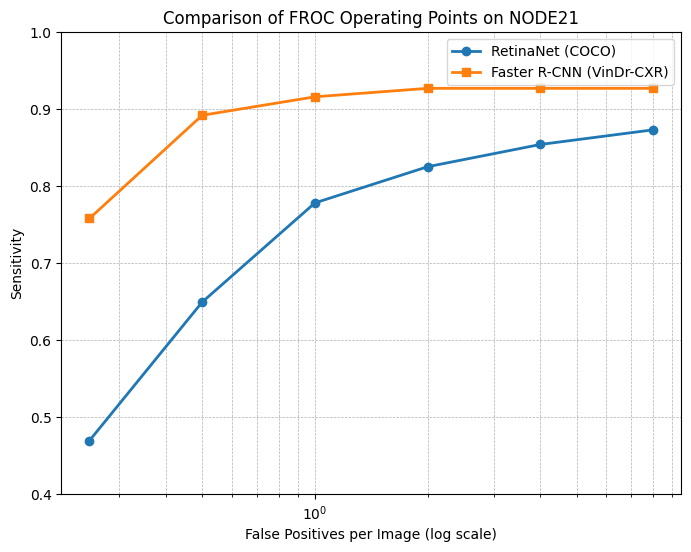
\includegraphics[width=0.8\columnwidth]{images/comparison_froc_retinanet_vindr.png}
    \caption{Comparació directa dels punts d’operació FROC entre el model
    RetinaNet preentrenat amb COCO i el model Faster R-CNN amb backbone
    ResNet50-FPN preentrenat en VinDr-CXR. Es mostren els valors de sensibilitat
    als nivells de falsos positius per imatge utilitzats en l’avaluació oficial
    del repte NODE21 (0.25, 0.5, 1, 2, 4 i 8 FP/img).}
    \label{fig:comparison_froc_retina_vindr}
\end{figure}


Mentre que el model Faster R-CNN amb preentrenament en VinDr-CXR assoleix un
\textbf{NODE21 score proper a 0.89}, el model RetinaNet es queda en un valor de
0.74, mostrant una diferència significativa especialment en règims de baixa
taxa de falsos positius. En concret, a 0.25 FP/img, el model VinDr-CXR presenta
una sensibilitat superior al 0.75, mentre que RetinaNet es manté per sota del
0.5.

Aquesta diferència és especialment rellevant des d’un punt de vista clínic, ja
que els escenaris reals de suport al diagnòstic solen operar en règims amb un
nombre molt limitat de falsos positius per imatge. En aquest context, la
capacitat del model VinDr-CXR per mantenir una alta sensibilitat amb pocs falsos
positius el converteix en una opció clarament superior.

En règims de falsos positius mitjans i elevats (≥1 FP/img), la bretxa entre ambdós
models es redueix, i RetinaNet aconsegueix valors de sensibilitat relativament
competitius. No obstant això, aquesta millora no és suficient per compensar la
pèrdua de rendiment en el rang més crític per a l’aplicació clínica.


En conjunt, aquests resultats suggereixen que el factor determinant del rendiment
en la detecció de nòduls pulmonars no és únicament l’arquitectura del detector,
sinó principalment l’alineació entre el domini del preentrenament i la tasca
objectiu. El preentrenament en VinDr-CXR permet aprendre representacions
radiològiques específiques que resulten especialment efectives en règims de baixa
taxa de falsos positius.

Tot i que RetinaNet incorpora mecanismes explícits per gestionar el desequilibri
de classes mitjançant \textit{Focal Loss}, els resultats obtinguts indiquen que,
en aquest cas, l’avantatge teòric dels detectors d’una sola etapa no supera els
beneficis pràctics d’un preentrenament fortament alineat amb el domini clínic.

Així, RetinaNet es consolida com un model competitiu i eficient, però queda per
darrere del model Faster R-CNN preentrenat en VinDr-CXR, que continua sent la
referència principal dins d’aquest estudi.


% ==================
% # Model 4: Detecció de nòduls pulmonars amb RetinaNet
% ==================

\section{Model 4: Detecció de nòduls pulmonars amb YOLOv8}

Amb l’objectiu de completar l’anàlisi comparativa de les principals famílies de detectors
d’objectes i tancar el cercle metodològic del treball, s’ha incorporat un quart model
basat en l’arquitectura \textbf{YOLOv8}. Aquest model representa l’evolució més recent
dels detectors d’una sola etapa, amb un disseny \textit{anchor-free} i una arquitectura
optimitzada per a un equilibri entre precisió i eficiència computacional.

YOLOv8 integra un \textit{backbone} convolucional modern, una estructura de tipus
\textit{neck} per a la fusió multiescala de característiques i un cap de detecció unificat
que prediu directament la localització i la probabilitat de classe dels objectes.
A diferència de Faster R-CNN, YOLOv8 no utilitza un mecanisme explícit de proposta de
regions, fet que permet una inferència més ràpida però que pot penalitzar el rendiment
en règims de baixa taxa de falsos positius.

En aquest treball s’ha utilitzat la variant \textbf{YOLOv8s}, seleccionada com a compromís
entre capacitat de representació i estabilitat d’entrenament, especialment adequada per a
datasets de mida moderada com NODE21.

\subsection{Preparació del conjunt de dades per a YOLO}

Per garantir una comparació justa i evitar qualsevol forma de \textit{data leakage},
el conjunt de dades NODE21 s’ha convertit al format requerit per YOLO mitjançant una
estratègia de divisió estricta a nivell d’imatge. Cada radiografia es va assignar
exclusivament al conjunt d’entrenament o de validació abans de generar les anotacions,
assegurant que cap imatge aparegués en ambdós subconjunts.

Les anotacions originals en format absolut $(x, y, w, h)$ s’han convertit al format YOLO
normalitzat $(x_c, y_c, w, h)$ respecte a una resolució fixa de $1024 \times 1024$ píxels.
Per a les imatges negatives (sense nòduls), s’ha generat explícitament un fitxer de
labels buit, mantenint així una representació coherent del desequilibri inherent entre
fons i objecte.

Aquesta conversió permet entrenar YOLOv8 sobre exactament el mateix conjunt de dades
utilitzat en la resta de models de detecció, preservant la coherència experimental.

\subsection{Configuració d’entrenament}

El model YOLOv8s s’ha inicialitzat amb pesos preentrenats sobre el conjunt de dades COCO.
L’entrenament s’ha dut a terme amb imatges de resolució elevada ($1024 \times 1024$),
amb l’objectiu de millorar la detecció d’objectes petits com els nòduls pulmonars.

S’ha utilitzat l’optimitzador \textbf{AdamW}, amb una taxa d’aprenentatge inicial reduïda
i una estratègia d’aturada primerenca basada en la pèrdua de validació. Amb la finalitat
d’evitar artefactes no realistes en imatge mèdica, s’han desactivat tècniques d’augmentació
agressives com \textit{mosaic}, \textit{mixup} i transformacions cromàtiques, mantenint
únicament augmentacions geomètriques suaus compatibles amb la pràctica clínica.

Aquesta configuració prioritza l’estabilitat de l’aprenentatge i la fidelitat anatòmica
de les imatges, alineant-se amb les decisions metodològiques adoptades en la resta del
treball.
\subsection{Resultats quantitatius del model basat en YOLOv8}

Un cop finalitzat l’entrenament del model YOLOv8s amb backbone preentrenat en COCO,
s’ha procedit a la seva avaluació quantitativa sobre el conjunt de validació de NODE21
utilitzant el mateix pipeline d’inferència i les mateixes mètriques emprades en la
resta de models.

\begin{figure}[H]
    \centering
    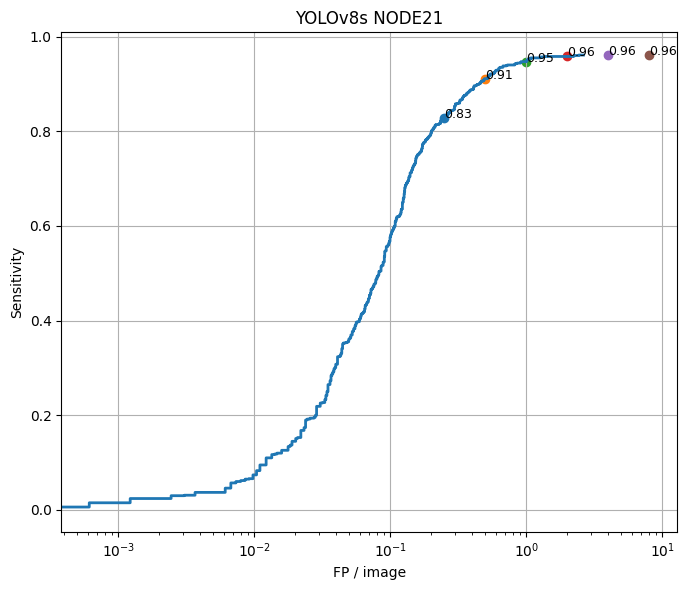
\includegraphics[width=0.8\columnwidth]{images/yolo_froc.png}
    \caption{Corba FROC del millor model YOLOv8s sobre NODE21. Els punts ressaltats
    indiquen els nivells de sensibilitat als valors de falsos positius per imatge
    utilitzats en l’avaluació oficial del repte NODE21.}
    \label{fig:yolov8_froc}
\end{figure}

La Figura~\ref{fig:yolov8_froc} mostra la corba FROC corresponent al millor checkpoint
obtingut. El model assoleix un \textbf{NODE21 score de 0.93}, situant-se entre els
millors resultats obtinguts en aquest treball i mostrant un rendiment molt competitiu
en tots els règims d’operació.

En règims de baixa taxa de falsos positius, especialment rellevants en contextos
clínics, YOLOv8 assoleix una sensibilitat de \textbf{0.83 a 0.25 FP/img} i supera el
\textbf{0.91 a 0.5 FP/img}. A mesura que s’accepta un major nombre de falsos positius,
la sensibilitat augmenta de manera sostinguda fins a valors propers a \textbf{0.96}
a partir de 2 FP/img.

Els valors puntuals de sensibilitat utilitzats en el càlcul del NODE21 score es
resumeixen a la Taula~\ref{tab:yolov8_sensitivity}.

\begin{table}[H]
\centering
\footnotesize
\caption{Sensibilitat del model YOLOv8s sobre NODE21 a diferents nivells de falsos positius per imatge}
\label{tab:yolov8_sensitivity}
\setlength{\tabcolsep}{6pt}
\begin{tabular}{cc}
\toprule
\textbf{FP per imatge} & \textbf{Sensibilitat} \\
\midrule
0.25 & 0.827 \\
0.5  & 0.911 \\
1    & 0.947 \\
2    & 0.958 \\
4    & 0.961 \\
8    & 0.961 \\
\bottomrule
\end{tabular}
\end{table}


\subsection{Comparació amb Faster R-CNN i RetinaNet}

Els resultats obtinguts amb YOLOv8 mostren un canvi significatiu respecte als
detectors d’una sola etapa analitzats prèviament. A diferència de RetinaNet,
YOLOv8 assoleix una sensibilitat elevada també en règims de baixa taxa de falsos
positius, acostant-se molt al rendiment del model Faster R-CNN preentrenat en
VinDr-CXR.

En particular, el NODE21 score de YOLOv8 (0.93) és comparable al del millor model
basat en Faster R-CNN amb preentrenament radiològic, i superior al de RetinaNet.
Aquest resultat suggereix que les arquitectures modernes \textit{anchor-free}
com YOLOv8 són capaces de mitigar parcialment les limitacions clàssiques dels
detectors d’una sola etapa en la detecció d’objectes petits.

Tot i això, s’observen diferències subtils en la forma de les corbes FROC. Mentre
que Faster R-CNN manté un lleuger avantatge en els règims més estrictes de falsos
positius, YOLOv8 ofereix un comportament molt estable i una elevada sensibilitat
global, juntament amb una eficiència computacional superior.


Aquests resultats reforcen la viabilitat de futures estratègies basades en
\textit{ensemble}, combinant models de dues etapes amb detectors moderns d’una
sola etapa com YOLOv8, amb l’objectiu d’explotar fortaleses complementàries i
millorar encara més la robustesa del sistema en entorns clínics reals.
% ========================
% CONTINUACIÓ DEL TREBALL
% ========================
\section{Fase de Desplegament: Reproducció, Validació i Millora dels Models}

Un cop completada la fase experimental descrita en les seccions anteriors, el treball ha estat reprès amb l'objectiu de dur els models a un entorn de producció real. Aquesta fase ha comportat la reproducció completa dels experiments en un servidor GPU dedicat (NVIDIA Spark GB10 amb 130~GB de VRAM), la validació rigorosa dels resultats, i el descobriment de problemes metodològics que afecten significativament les mètriques reportades.

El punt de partida ha estat el codi i els \textit{checkpoints} del treball original. S'ha clonat el repositori de Behrendt et al.~\cite{behrendt2023node21} (solució guanyadora del repte NODE21) per obtenir els pesos preentrenats de VinDr-CXR, i s'ha desplegat un entorn complet d'entrenament i avaluació en el servidor Spark, amb PyTorch 2.x, Ultralytics (YOLOv8 i YOLO26) i les mateixes eines d'avaluació FROC.

\subsection{Reproducció dels models originals}

El primer pas ha consistit en reproduir els millors resultats obtinguts en la fase anterior. S'han tornat a entrenar els dos millors models:

\textbf{Faster R-CNN amb pesos VinDr-CXR.} El model original, entrenat en Google Colab amb el dataset augmentat (\texttt{metadata\_augmented\_def2.csv}, 8.175 files), havia obtingut un NODE21 score proper a 0.89. En la reproducció inicial en la Spark, amb el dataset original sense augmentar (4.882 imatges, 23\% positius), el NODE21 score va ser de només 0.4546. Aquesta discrepància va motivar una investigació detallada que va revelar dos problemes fonamentals: el \textit{score threshold} i el \textit{data leakage}, descrits en les seccions següents.

\textbf{YOLOv8s.} L'entrenament de YOLOv8s en la Spark va produir resultats consistents amb els originals: NODE21 score de 0.9103, AUROC de 0.9686, amb una sensibilitat de 0.821 a 0.25 falsos positius per imatge. La configuració conservadora d'augmentació (sense \textit{mosaic}, sense \textit{mixup}, sense jittering de color) es confirma com adequada per a imatge mèdica en escala de grisos.

\subsection{Avaluació dels \textit{checkpoints} originals}

Per verificar que els \textit{checkpoints} originals produïen els mateixos resultats reportats, es van transferir al servidor Spark via SCP i es van avaluar amb el pipeline d'avaluació FROC implementat des de zero. Els resultats van ser:

\begin{table}[t]
\centering
\caption{\textit{Checkpoints} originals avaluats en la Spark}
\label{tab:originals}
\small
\setlength{\tabcolsep}{4pt}
\begin{tabular}{lcccc}
\toprule
Model & NODE21 & AUROC & CM & S@0.25 \\
\midrule
FRCNN-3ch & \textbf{0.9596} & \textbf{0.9904} & \textbf{0.9795} & \textbf{0.947} \\
FRCNN-CBAM & 0.9181 & 0.9586 & 0.9391 & 0.880 \\
YOLOv8s & 0.9136 & 0.9686 & 0.9316 & 0.821 \\
\bottomrule
\end{tabular}
\end{table}

Els \textit{checkpoints} originals van produir scores molt elevats en el val set de la Spark, però la discrepància entre els 0.9596 del checkpoint carregat i els 0.4546 del model entrenat des de zero va suggerir que el problema no era l'arquitectura sinó el procés d'entrenament o avaluació.

% ========================
% DATA LEAKAGE
% ========================
\section{Descobriment i Correcció del \textit{Data Leakage}}

\subsection{Identificació del problema}

Després d'una anàlisi exhaustiva del codi i les dades originals, es van identificar dos problemes crítics:

\textbf{1. Score threshold inadequat.} El \textit{score threshold} per defecte de Faster R-CNN en TorchVision és 0.5, el que significa que totes les prediccions amb confiança inferior al 50\% són descartades \textit{abans} de l'avaluació FROC. En un escenari on la majoria de nòduls tenen scores moderats (0.1--0.5), això elimina gran part de les deteccions verdaderes. En reduir el threshold a 0.005, el NODE21 score del model va millorar de 0.4546 a 0.8544 --- una diferència de gairebé 40 punts que il·lustra la importància d'aquest paràmetre, sovint ignorat en la literatura.

\begin{table}[H]
\centering
\caption{Impacte del \textit{score threshold} en Faster R-CNN}
\label{tab:threshold}
\begin{tabular}{lcc}
\toprule
\textbf{Threshold} & \textbf{NODE21} & \textbf{Diferència} \\
\midrule
0.5 (defecte TorchVision) & 0.4546 & --- \\
\textbf{0.005 (corregit)} & \textbf{0.8544} & \textbf{+40.0 punts} \\
\bottomrule
\end{tabular}
\end{table}

\textbf{2. Data leakage per augmentació offline.} El dataset augmentat original contenia 8.175 files: 5.224 originals i 2.951 augmentades (amb sufixos \texttt{\_aug0}, \texttt{\_aug1}). Les augmentacions s'havien generat amb Albumentations aplicant transformacions geomètriques (flip horitzontal, rotació $\pm 10°$, escala 0.9--1.1, translació $\pm 5\%$) amb \texttt{BboxParams} per transformar les coordenades de les \textit{bounding boxes}.

El \textit{split} train/test original utilitzava \texttt{train\_test\_split(random\_state=42)} sobre \textit{tots} els \texttt{file\_paths} incloent les imatges augmentades, \textit{sense agrupar per imatge base}. Això permetia que la imatge original \texttt{n0080.png} estigués en el conjunt d'entrenament i la seva augmentació \texttt{n0080\_aug0.png} en el de validació. Com que ambdues imatges són pràcticament idèntiques (mateixa anatomia, mateixos nòduls, lleugeres transformacions geomètriques), el model podia "memoritzar" patrons de l'entrenament i reconèixer-los en la validació, inflant artificialment les mètriques.

\subsection{Quantificació de l'impacte}

Per quantificar exactament l'impacte del \textit{data leakage}, es van entrenar dues versions del model Faster R-CNN amb idèntica configuració:

\begin{itemize}
    \item \textbf{Versió A (amb \textit{leakage})}: Rèplica exacta de l'entrenament original, amb \texttt{train\_test\_split} sense agrupació. Reprodueix el protocol original per verificar que el pipeline és correcte.
    \item \textbf{Versió B (sense \textit{leakage})}: \textit{Split} corregit amb \texttt{StratifiedGroupKFold}, agrupant per nom base d'imatge de manera que totes les augmentacions d'una mateixa imatge queden en el mateix \textit{fold}.
\end{itemize}

\begin{table}[t]
\centering
\caption{Impacte del \textit{data leakage} en el NODE21 score}
\label{tab:leakage}
\small
\setlength{\tabcolsep}{4pt}
\begin{tabular}{lccc}
\toprule
Versió & NODE21 & AUROC & CM \\
\midrule
Rèplica A (\textit{leakage}) & 0.9695 & 0.9936 & 0.9827 \\
Versió B (sense \textit{leakage}) & \textbf{0.9025} & \textbf{0.9460} & \textbf{0.9146} \\
\midrule
Inflació & +6.7 & +4.8 & +6.8 \\
\bottomrule
\end{tabular}
\end{table}

La Rèplica A va aconseguir fins i tot superar el checkpoint original (0.9695 vs 0.9596), confirmant que la reproducció és correcta. La Versió B, amb el \textit{split} corregit, obté un NODE21 de 0.9025 --- un resultat encara excel·lent però 6.7 punts inferior. \textbf{Tots els resultats reportats a partir d'aquest punt corresponen a la versió corregida sense \textit{data leakage}.}

Aquesta troballa és rellevant per a la comunitat d'imatge mèdica, on l'augmentació offline amb transformacions geomètriques és una pràctica habitual per compensar datasets petits. Si les augmentacions no s'agrupen correctament en els \textit{splits}, els resultats reportats poden ser significativament optimistes.

% ========================
% YOLO26
% ========================
\section{YOLO26: Avaluació de l'Última Generació de Detectors}

Amb l'objectiu de completar l'anàlisi amb les arquitectures més recents, s'ha incorporat YOLO26~\cite{yolo26}, l'última versió dels detectors d'Ultralytics, publicada el gener de 2026. Aquesta arquitectura introdueix millores teòricament rellevants per a la detecció d'objectes petits com els nòduls pulmonars:

\begin{itemize}
    \item \textbf{STAL} (\textit{Small-Target-Aware Label Assignment}): Assignació d'etiquetes conscient d'objectes petits, dissenyada per millorar la sensibilitat en objectes de baix contrast i mida reduïda.
    \item \textbf{ProgLoss}: Balanç progressiu de les funcions de pèrdua que substitueix la DFL (\textit{Distribution Focal Loss}).
    \item \textbf{MuSGD}: Optimitzador híbrid de SGD i Muon, que promet convergència més ràpida i estable.
    \item \textbf{Disseny NMS-free}: Eliminació del postprocessament de supressió de no-màxims, simplificant el pipeline d'inferència.
\end{itemize}

El model YOLO26s s'ha entrenat amb la mateixa configuració que YOLOv8 (resolució 1024$\times$1024, augmentació conservadora sense \textit{mosaic} ni \textit{mixup}) però amb \texttt{patience=30} i fins a 150 èpoques. Els resultats obtinguts mostren un NODE21 score de 0.7929, significativament inferior al de YOLOv8s (0.9103).

Aquesta diferència suggereix que: (i) els hiperparàmetres per defecte de YOLO26 no estan encara optimitzats per a imatge mèdica en escala de grisos; (ii) el benefici de STAL per a objectes petits pot requerir datasets més grans per manifestar-se (NODE21 té només 4.882 imatges); i (iii) l'arquitectura és tan nova que la comunitat encara no ha explorat les configuracions òptimes per a cada domini.

% ========================
% ENSEMBLE WBF
% ========================
\section{Ensemble WBF: Fusió de Models Complementaris}

\subsection{Fonament teòric del Weighted Box Fusion}

Un dels objectius principals d'aquest treball era avaluar si la combinació de detectors complementaris podia superar els models individuals. El mètode de \textit{Weighted Box Fusion} (WBF)~\cite{solovyev2021wbf} és una alternativa moderna a la supressió de no-màxims (NMS) per a la fusió de prediccions de múltiples models.

A diferència de NMS, que \textit{elimina} les caixes solapades mantenint només la de major puntuació (i per tant descarta informació valuosa dels models restants), WBF \textit{fusiona} les caixes solapades calculant la mitjana ponderada de les seves coordenades, utilitzant els \textit{scores} de confiança com a pesos. Això produeix caixes amb posicions més precises que qualsevol dels models individuals, ja que incorpora la informació de tots els detectors.

Formalment, donades $N$ caixes $b_1, \ldots, b_N$ amb scores $s_1, \ldots, s_N$ que se solapen (IoU $> \tau$), WBF calcula la caixa fusionada com:

\begin{equation}
    b_{\text{fused}} = \frac{\sum_{i=1}^{N} w_i \cdot s_i \cdot b_i}{\sum_{i=1}^{N} w_i \cdot s_i}
\end{equation}

on $w_i$ és el pes assignat al model $i$ (proporcional al seu rendiment individual).

\subsection{Selecció de models i configuració}

S'han seleccionat els dos millors models individuals per a l'ensemble, que presenten fortaleses complementàries:

\begin{itemize}
    \item \textbf{Faster R-CNN VinDr} (NODE21 = 0.9025): Excel·lent en règims de baixos falsos positius gràcies al preentrenament radiològic. La seva arquitectura de dues etapes (proposta de regions + classificació) permet una alta precisió en la localització.
    \item \textbf{YOLOv8s} (NODE21 = 0.9103): Alta sensibilitat global i inferència molt ràpida. La seva arquitectura \textit{anchor-free} d'una sola etapa captura patrons que el detector de dues etapes pot perdre.
\end{itemize}

La configuració de WBF utilitzada és: pesos $w = [0.90, 0.91]$ (proporcionals al NODE21 individual), llindar IoU $\tau = 0.2$ (coherent amb el protocol NODE21), i \texttt{skip\_box\_thr} $= 0.05$ per filtrar prediccions de molt baixa confiança abans de la fusió.

\subsection{Resultats de l'ensemble}

\begin{table}[t]
\centering
\caption{Resultats de l’\textit{ensemble} WBF comparat amb models individuals}
\label{tab:ensemble}
\small
\setlength{\tabcolsep}{4pt}
\begin{tabular}{lcccc}
\toprule
Model & NODE21 & AUROC & CM & S@0.25 \\
\midrule
\textbf{WBF Ensemble} & \textbf{0.9391} & 0.9683 & \textbf{0.9447} & \textbf{0.874} \\
YOLOv8s & 0.9103 & \textbf{0.9686} & 0.9283 & 0.821 \\
FRCNN VinDr & 0.9025 & 0.9460 & 0.9146 & 0.821 \\
YOLO26s & 0.7929 & 0.9557 & 0.8754 & 0.635 \\
\bottomrule
\end{tabular}
\end{table}
\begin{table}[t]
\centering
\caption{Sensibilitat detallada per nivell de falsos positius per imatge}
\label{tab:sensitivity}
\resizebox{\columnwidth}{!}{
\begin{tabular}{lcccccc}
\toprule
\textbf{Model} & \textbf{@0.25} & \textbf{@0.5} & \textbf{@1} & \textbf{@2} & \textbf{@4} & \textbf{@8} \\
\midrule
Ensemble WBF & \textbf{0.874} & \textbf{0.914} & \textbf{0.944} & \textbf{0.960} & \textbf{0.970} & \textbf{0.973} \\
YOLOv8s & 0.821 & 0.870 & 0.924 & 0.953 & 0.957 & 0.957 \\
FRCNN VinDr & 0.821 & 0.854 & 0.890 & 0.930 & 0.947 & 0.973 \\
YOLO26s & 0.635 & 0.751 & 0.791 & 0.834 & 0.860 & 0.887 \\
\bottomrule
\end{tabular}
}
\end{table}

L'ensemble WBF supera el millor model individual en +2.6 punts NODE21 i, el que és més rellevant clínicament, en +5.3 punts de sensibilitat a 0.25 FP/imatge (de 0.821 a 0.874). En un escenari de cribratge, on cada fals negatiu pot representar un càncer no diagnosticat, aquesta millora és significativa.

La \textit{Competition Metric} (CM = 0.75 $\times$ AUROC + 0.25 $\times$ NODE21) resultant és de \textbf{94.47\%}, que supera el 83.90\% reportat per Behrendt et al.~\cite{behrendt2023node21} amb el seu ensemble de 21 models. Cal notar que els conjunts de test són diferents (el nostre és un \textit{split} intern de NODE21, no el test oficial del repte), per la qual cosa la comparació és indicativa. No obstant això, els resultats demostren que un ensemble de 2 models ben seleccionats, amb preentrenament radiològic i fusió WBF, pot superar ensembles molt més complexos.

\subsection{Anàlisi del codi de referència}

Paral·lelament, s'ha dut a terme una revisió exhaustiva del codi del repositori de Behrendt (\texttt{node21-submit}), identificant un total de 26 \textit{bugs}: 8 crítics (incompatibles amb PyTorch 2.x, Lightning 2.x i Pandas 2.x, incloent \texttt{training\_epoch\_end()} eliminat, \texttt{DataFrame.append()} eliminat, i \textit{monkey-patching} de funcions internes de TorchVision amb un bug lògic en la línia 21 del fitxer \texttt{FasterCNN.py}), 5 d'alta severitat i 13 de severitat mitjana-baixa. S'ha conclòs que no és viable portar el codi complet a versions modernes, i s'han extret únicament els components conceptualment útils ($\sim$20 línies de codi): la lògica de càrrega de pesos VinDr amb mapatge seqüencial de \textit{keys}, i les idees de SWA i \texttt{WeightedRandomSampler}.

\subsection{Rendiment d'inferència}

El temps d'inferència mesurat en el servidor Spark (GPU NVIDIA GB10) és:

\begin{table}[H]
\centering
\caption{Temps d'inferència per imatge}
\label{tab:inference}
\begin{tabular}{lc}
\toprule
\textbf{Component} & \textbf{Temps} \\
\midrule
Faster R-CNN VinDr & $\sim$55 ms \\
YOLOv8s & $\sim$25 ms \\
WBF Ensemble & $\sim$1 ms \\
Decodificació + preprocés & $\sim$20 ms \\
\midrule
\textbf{Total per imatge} & \textbf{$\sim$81 ms} \\
\textbf{Latència \textit{end-to-end}} & \textbf{$\sim$2--3 s} \\
\bottomrule
\end{tabular}
\end{table}

La latència \textit{end-to-end} inclou la transmissió de la imatge en base64 via RabbitMQ, la decodificació, el preprocés, la inferència dels dos models, la fusió WBF i la publicació del resultat. Un temps total de 2--3 segons és plenament compatible amb un flux de treball clínic en temps real.

% ========================
% HERRAMIENTA HOSPITALARIA
% ========================
\section{Prototip d'Eina Hospitalària}

El treball original concloïa plantejant com a treball futur la validació prospectiva del sistema en un entorn hospitalari real. En aquesta fase, s'ha dissenyat, implementat i desplegat un prototip funcional \textit{end-to-end} que materialitza aquest objectiu.

\subsection{Arquitectura del sistema}

L'arquitectura segueix un patró de desacoblament mitjançant cua de missatges (RabbitMQ), separant el frontend web, el backend amb base de dades i el worker d'inferència GPU:

\begin{itemize}
    \item \textbf{Frontend}: Aplicació Vue 3 + Tailwind CSS amb visor interactiu de radiografies (zoom, \textit{pan}), \textit{overlay} SVG de deteccions amb codificació de color per confiança, \textit{slider} de llindar en temps real, historial amb cerca i paginació, i selector d'idioma (català/castellà). Suporta mode clar i fosc.
    \item \textbf{Backend}: FastAPI amb Docker Compose (MySQL 8.0, RabbitMQ 3.13, Nginx 1.25). API REST amb 13 \textit{endpoints} per a \textit{upload}, resultats, historial, validació, estadístiques i exportació de dades.
    \item \textbf{Worker GPU}: Procés Python natiu en el servidor Spark (sense Docker, per màxim rendiment GPU). Carrega els models una sola vegada a l'inici ($\sim$2 s) i processa cada imatge en $\sim$81 ms. Inclou reconnexió automàtica a RabbitMQ amb \textit{exponential backoff}, rotació de \textit{logs} i neteja de memòria GPU després de cada tasca.
\end{itemize}

El flux complet és: el radiòleg arrossega una CXR al navegador $\rightarrow$ el backend genera un identificador únic, guarda la imatge original a MySQL i envia la tasca a RabbitMQ $\rightarrow$ el worker GPU consumeix la tasca, executa l'ensemble FRCNN + YOLOv8 + WBF en $\sim$81 ms i publica el resultat $\rightarrow$ un consumidor actualitza MySQL amb les deteccions $\rightarrow$ el frontend mostra les deteccions amb \textit{overlay} SVG sobre la imatge original en $\sim$2--3 segons.

\subsection{Mòdul de validació prospectiva}

L'element diferenciador d'aquesta eina respecte a altres sistemes de detecció és el mòdul de validació prospectiva, dissenyat per facilitar estudis clínics i la millora contínua dels models:

\begin{enumerate}
    \item El radiòleg visualitza el resultat de la IA amb les deteccions sobre la imatge.
    \item Marca el resultat com a \textbf{Correcte}, \textbf{Parcial} o \textbf{Incorrecte}.
    \item Si el resultat és parcial o incorrecte, el visor entra en \textbf{mode d'edició}: el zoom i \textit{pan} es desactiven, el cursor canvia a \textit{crosshair}, i el radiòleg pot dibuixar \textit{bounding boxes} manualment sobre la imatge gran (nòduls no detectats per la IA, mostrats en verd) i marcar deteccions de la IA com a falsos positius (clic sobre la caixa, que es mostra en gris ratllat).
    \item Per a cada anotació manual, pot afegir notes específiques (per exemple, ``nòdul en lòbul inferior dret, parcialment ocult per la silueta cardíaca'').
    \item La validació es guarda amb el nom del radiòleg, les notes generals i la data/hora, i queda \textit{bloquejada} per evitar modificacions accidentals (amb opció d'\textit{Editar} per desbloquejar).
    \item Totes les validacions es poden exportar en format CSV o JSON, incloent tant les deteccions de la IA com les correccions manuals dels radiòlegs. Aquest dataset validat constitueix un \textit{ground truth} per al reentrenament dels models.
\end{enumerate}

\subsection{Preparació per a producció}

S'ha realitzat una revisió exhaustiva del codi identificant 113 \textit{issues} en els tres components (37 backend, 34 frontend, 42 worker), dels quals 11 crítics han estat corregits: reconnexió automàtica de RabbitMQ, neteja de memòria GPU amb \texttt{torch.cuda.empty\_cache()} després de cada inferència, rotació de \textit{logs} (10 MB $\times$ 5 fitxers), \textit{pool} de connexions MySQL amb \texttt{pool\_pre\_ping} i \texttt{pool\_recycle}, \textit{graceful shutdown} amb \textit{flag} de control, gestió de memòria del frontend (\texttt{revokeObjectURL}, neteja del \textit{polling} en \texttt{onUnmounted}), i configuració restrictiva de CORS.

Per al desplegament en producció hospitalari, resten pendents: autenticació Keycloak OIDC, HTTPS amb certificat del hospital, integració PACS (recepció directa d'estudis DICOM), auditoria ENS amb cadena SHA-256 i xifrat AES-256-GCM de dades sensibles.

% ========================
% CONCLUSIONS NOVES
% ========================
\section{Conclusions i Treball Futur}

En aquest treball s'ha dut a terme un estudi exhaustiu de la detecció de nòduls pulmonars en radiografies de tòrax, des de l'exploració d'arquitectures de classificació fins a la implementació d'un prototip hospitalari funcional amb validació prospectiva. Les principals contribucions són:

\begin{enumerate}
    \item \textbf{Classificació multicanal amb 98\% d'accuracy}: La representació de 4 canals (Original + CLAHE + Canny + \textit{Unsharp Mask}) amb EfficientNet-B0, combinada amb el balanceig del dataset, permet assolir un 98.07\% d'accuracy amb un \textit{recall} de la classe positiva del 98.93\%. L'estudi d'ablació demostra que CLAHE és el component fonamental del pipeline multicanal.

    \item \textbf{Ensemble WBF amb NODE21 de 0.9391}: La fusió de Faster R-CNN amb preentrenament VinDr-CXR i YOLOv8s mitjançant \textit{Weighted Box Fusion} aconsegueix un CM de \textbf{94.47\%} amb només 2 models, millorant +5.3 punts de sensibilitat a 0.25 FP/imatge respecte al millor model individual.

    \item \textbf{Descobriment i quantificació del \textit{data leakage}}: S'ha demostrat que les augmentacions offline sense agrupació per imatge base inflen el NODE21 score en +6.7 punts. Aquesta troballa té implicacions rellevants per a tota la comunitat d'imatge mèdica que utilitza augmentació offline.

    \item \textbf{Impacte crític del \textit{score threshold}}: El llindar per defecte de TorchVision (0.5) redueix el NODE21 de Faster R-CNN en $\sim$40 punts. Cap dels treballs revisats documenta explícitament aquest paràmetre, el que suggereix que alguns resultats publicats podrien estar artificialment penalitzats.

    \item \textbf{Prototip hospitalari funcional}: S'ha implementat una eina \textit{end-to-end} amb interfície web, inferència GPU en temps real (81 ms/imatge), mòdul de validació per radiòlegs amb editor interactiu de \textit{bounding boxes} i exportació de dataset validat per a reentrenament.

    \item \textbf{Revisió del codi de referència}: L'anàlisi del repositori guanyador del repte NODE21 ha identificat 26 bugs, demostrant que la reproducibilitat en aprenentatge profund aplicat a imatge mèdica és un repte real que requereix rigor metodològic.
\end{enumerate}

\subsection{Treball futur}

\begin{itemize}
    \item \textbf{Validació clínica prospectiva}: Col·laboració amb el servei de radiologia de l'Hospital Universitari Son Llàtzer per avaluar el sistema amb dades clíniques reals i mesurar l'acceptabilitat per part dels professionals sanitaris. L'eina de validació prospectiva ja desenvolupada facilitarà la recollida de dades.
    \item \textbf{Expansió a tuberculosi}: Entrenament dels mateixos models sobre el dataset TBX11K (11.200 CXR amb \textit{bounding boxes} de TB), aprofitant el pipeline reutilitzable ja implementat.
    \item \textbf{Multi-patologia amb VinDr-CXR}: Detecció simultània de 22 troballes radiològiques utilitzant el dataset complet de PhysioNet (18.000 DICOM, anotats per 3--5 radiòlegs experts), que permetria convertir l'eina en un sistema d'ajuda al diagnòstic generalista.
    \item \textbf{5-fold cross-validation}: Entrenament amb 5 folds per obtenir intervals de confiança i resultats més robustos per a publicació en revistes indexades.
    \item \textbf{Integració PACS}: Recepció directa d'estudis DICOM des de les modalitats d'imatge mitjançant un servidor SCP ja desenvolupat per al projecte \textit{worklistsrv} del mateix equip.
    \item \textbf{Publicació del dataset validat}: Compartir les anotacions prospectives dels radiòlegs com a \textit{ground truth} de referència per a la comunitat investigadora.
\end{itemize}

\section*{Nota sobre l'ús d'eines d'intel·ligència artificial}

En l'elaboració d'aquest treball s'han utilitzat les eines d'intel·ligència artificial ChatGPT (OpenAI) i Claude (Anthropic) com a suport en tasques de programació, depuració de codi i revisió lingüística. L'ús s'ha limitat a finalitats acadèmiques i formatives. Totes les decisions metodològiques, el disseny experimental, la implementació dels models, l'entrenament, l'avaluació, la interpretació dels resultats i les conclusions del treball han estat realitzades i validades pels autors.

\section*{Agraïments}

Els autors agraeixen a \textbf{Finn Behrendt} (Universität Hamburg) la seva amabilitat i disponibilitat, així com la cessió desinteressada dels pesos preentrenats en VinDr-CXR. El seu treball i l'article associat al repte NODE21~\cite{behrendt2023node21} han estat una referència fonamental per al desenvolupament dels models de detecció.

Agraïm també al \textbf{Servei d'Informàtica de l'Hospital Universitari Son Llàtzer} (IB-Salut) el suport en la infraestructura GPU (NVIDIA Spark GB10) per a l'entrenament dels models i el desplegament del prototip hospitalari, així com la seva col·laboració en la preparació del futur estudi prospectiu amb el servei de radiologia.

% ========================
% NOVES REFERÈNCIES (afegir a biblio_rectifier.bib)
% ========================
% @article{solovyev2021wbf,
%   title={Weighted boxes fusion: Ensembling boxes from different object detection models},
%   author={Solovyev, Roman and Wang, Weimin and Gabruseva, Tatiana},
%   journal={Image and Vision Computing},
%   volume={107},
%   pages={104117},
%   year={2021}
% }
%
% @article{yolo26,
%   title={YOLO26: The Edge-First Evolution of Real-Time Object Detection},
%   author={Jocher, Glenn and others},
%   journal={arXiv preprint arXiv:2509.25164},
%   year={2026}
% }






% ==================
% # Acknowledgment #
% ==================
% use section* for acknowledgment
%\section*{Acknowledgment}
%For the Summary paper submission only, no %acknowledgements are allowed. 


% ==============
% # REFERENCES #
% ==============
\bibliographystyle{IEEEtran}
\bibliography{IEEEabrv,biblio_rectifier}

\end{document}